\documentclass[12pt,letterpaper,oneside]{book}

\usepackage{listings}
\usepackage{graphicx}
\usepackage{subfigure}
\usepackage{pdflscape}
\usepackage{captcont}
\usepackage{setspace}
\usepackage{url}
\usepackage{fancyhdr}
\usepackage{textcomp}
\usepackage{longtable}
\usepackage[page,titletoc]{appendix}
\usepackage{amsmath}
\usepackage{amssymb}
\usepackage[mathscr]{eucal}
\usepackage{algorithm}
\usepackage{algorithmic}
\usepackage{array}
\usepackage[Sonny]{fncychap}
\usepackage[top=1in, bottom=1in, left=1.5in, right=1in, includefoot]{geometry}
\usepackage[pdftex,bookmarks=true]{hyperref}
\hypersetup{ linkbordercolor={1 1 1},citebordercolor={1 1 1} } 

\pagestyle{fancy}

\begin{document}

\onehalfspacing
\lstset{language=C}

% Define the header
\fancyhead{}
\rhead{\footnotesize{\emph{Texas Tech University, Bryan Hughes, May 2010}}}
\renewcommand{\headrulewidth}{0pt}
\renewcommand{\footrulewidth}{0pt}

% Note: we must redefine the plain style, because chapter headings automatically revert to plain style irregardless of other definitions
\fancypagestyle{plain}{%
\fancyhead{}
\rhead{\footnotesize{\emph{Texas Tech University, Bryan Hughes, December 2009}}}
\renewcommand{\headrulewidth}{0pt}
\renewcommand{\footrulewidth}{0pt}%
}


\frontmatter
\begin{titlepage}
\begin{centering}

\LARGE An Oblivious Routing Scheme for Parallel Computing in General Embedded Networks

\vspace{18pt}

\normalsize by\\

\vspace{8pt}

\large Bryan Hughes, B.S.E.E., M.S.E.E.\\

\vspace{18pt}

\normalsize A Dissertation \\

\vspace{8pt}

In\\

\vspace{8pt}

Electrical Engineering\\

\vspace{18pt}

Submitted to the Graduate Faculty\\
of Texas Tech University in\\
Partial Fulfillment of\\
the Requirements for\\
the Degree of\\

\vspace{18pt}

Doctor of Philosophy\\

\vspace{18pt}

Approved\\

\vspace{8pt}

Dr. Brian Nutter\\

\vspace{8pt}

Dr. Per Andersen\\

\vspace{8pt}

Dr. Ranadip Pal\\

\vspace{8pt}

Dr. Daniel Cooke\\

\vspace{8pt}

Dr. Sunanda Mitra\\

\vspace{18pt}

Fred Hartmeister\\
Dean of the Graduate School\\

\vspace{18pt}

May, 2010\\

\end{centering}
\end{titlepage}

\vspace*{\fill}
\begingroup
\centering
\thispagestyle{empty}

Copyright 2010, Bryan Hughes

\endgroup
\vspace*{\fill}

\chapter{Acknowledgements}
I would like to thank my dissertation advisor Dr. Nutter for his support of my project. His continual guidance has helped keep my project on track, and has given me countless inspirations for my project. I would also like to thank Dr. Andersen and Dr. Cooke for introducing me to so many interesting topics in Computer Science that were incorporated in my project. My thanks also extend to Dr. Mitra and Dr. Pal for their support of my project. Elliot Briggs, a fellow graduate student in Electrical Engineering, also has my thanks for his help in assembling the hardware in the project.

I would like to thank the Electrical and Computer Engineering department and Dr. Mitra for their financial support over the years, without which I would not have been able to achieve all that I have achieved. 

I am very grateful for the support of my friends and family over the years. They have always shown support for my endeavors and encouraged me to reach my highest potential. To my loving wife, Melissa; I am so lucky to have such a wonderful wife who put up with my long hours, constant prattling about my project, and always supported me.


\tableofcontents

\chapter{Abstract}
Parallel computing is currently undergoing a transition from a niche use to widespread acceptance because of the recent availability of multi-core processors in the personal computing market. These processors have given new levels of performance to desktop applications, allowing algorithms that were once the domain of supercomputers to now be run on home systems. The embedded world has yet to embrace these parallel systems except in ultra-high-end systems. Network performance is critical in parallel computing, and the routing algorithm has a direct impact on performance. In this dissertation, a prototype toolkit is developed consisting of five primary parts: a prototype router implemented using TI F2808 DSP controllers, a physical and data link layer that utilizes SPI as a base, a network layer protocol stack for handling transmission across a network, a routing algorithm, and an API that simplifies the programming of parallel algorithms. The routing algorithm is based on the seminal work of Harald R\"acke. R\"acke's method is very good at avoiding congestion, but is generally too complex for embedded systems. The algorithm presented here is a modified version of R\"acke's method that is more suitable for embedded systems while maintaining most of the advantages of R\"acke's method.

\listoftables
\addcontentsline{toc}{chapter}{List of Tables}

\listoffigures
\addcontentsline{toc}{chapter}{List of Figures}


\mainmatter

\chapter{Introduction}\label{sec:introduction}

Parallel and distributed computing has been utilized for decades in the high performance computing market as a means to increase performance. Parallel computing went mainstream in 2005 with the release of the first dual-core desktop processors. Almost every computer that is built today contains a multi-core processor, and many common software packages utilize parallel processing in day to day tasks. The embedded market, however, has yet to embrace parallel computing in any meaningful way. One method for utilizing parallel computing in embedded systems is to use a network of single-core embedded processors. Although the hardware already exists to implement such a network, the communications technology necessary for these processors to communicate does not yet exist. Most aspects of network communications technology are essentially solved problems, but routing has proven to be a difficult and elusive problem to solve when optimizing for distributed systems. This paper presents a prototype toolkit for embedded parallel and distributed computing that showcases a non-deterministic oblivious routing scheme that has been tailored for embedded systems.

\section{Parallel Video Transcoder - A Motivating Story}\label{sec:introduction:motivating_story}

A presentation was given at the Texas Instruments Developer Conference in 2007 titled ``A Scalable Multi-DM642-based MPEG-2 to H.264 Transcoder.'' \cite{ref:2007-raman-h.264_parallel_transcoder} The talk described a system for transcoding high definition video content encoded using the older MPEG-2 video codec to the newer H.264 video codec in real-time, a process that is too resource intensive for a single embedded processor. The system was designed to use multiple Texas Instruments DM642 Digital Signal Processors (DSPs) to cope with these requirements. 

The presenter spent much of the presentation discussing the mechanisms that were implemented to handle the communication and work sharing between DSPs. The results obtained with a two DSP system showed that they could only encode video with 75\% of the resolution of standard definition video! This equates to roughly 15\% of the resolution of a 1080p high definition video signal. Why could the end product only handle 15\% of the target goal? It can be inferred from the presentation that the developers spent much of their time setting up the basic mechanisms necessary to distribute the work load between two DSPs, instead of working on getting the algorithm to scale well to multiple DSPs. The presentation also informed the audience that the distribution mechanisms were very special-purpose, and modifying them to support more processors (or other applications) involved non-trivial modifications.

If the developers of the transcoding system had a toolkit that provided all of the basic mechanisms, including a high-performance routing algorithm, then perhaps they would have presented results showing a complete system. Such a toolkit could have also resulted in a faster time to market, and less cost in terms of engineering overhead, and one of the core components of the toolkit is the routing algorithm. It also illustrates that a complete toolkit is necessary for the development of a routing algorithm, and so a prototype toolkit is presented here that addresses the networking requirements necessary to perform routing in addition to the routing algorithm itself.

\section{Basics of Parallel and Distributed Computing}\label{sec:introduction:parallel_computing_overview}

Parallel computing is defined as dividing a program into sub-components that are executed simultaneously with the intent of decreasing execution time. Distributed computing is subtly different from parallel computing and is defined as utilizing a group of discrete processing elements to collaboratively solve a problem. A parallel computing system is often, but not always, a distributed computing system. Likewise, a distributed computing system is often, but not always, used for parallel computing. Parallel computing was initially employed in supercomputers to achieve higher performance levels. It has only been in the last few years that parallel computing has begun to appear in consumer level computers with the advent of multi-core processors. 

\subsection{Data and Processes}\label{sec:introduction:parallel_computing_overview:data_and_processes}

Computing systems can be defined using Flynn's Taxonomy, which states that all systems consist of \emph{instructions} and \emph{data} and that each can be defined as either \emph{single} or \emph{multiple}. \cite{ref:2009-barney-introduction_to_parallel_computing}

Single Instruction, Single Data (SISD) defines a serial computing system. A SISD system consists of a single processor that can only execute a single instruction at a time, and instructions can only work on a single piece of data at a time, as shown in Figure \ref{fig:introduction:sisd}.

\begin{figure}[ptb]
	\begin{centering}
		\includegraphics{Introduction/Figures/introduction-sisd.pdf}
		\caption{SISD Execution}
		\label{fig:introduction:sisd}
	\end{centering}
\end{figure}

Single Instruction, Multiple Data (SIMD) defines a computing system that executes the same instruction on several data elements at the same time, as shown in Figure \ref{fig:introduction:simd}.  This type of parallel computing is often employed when working with vectorized data, such as in image processing.

\begin{figure}[ptb]
	\begin{centering}
		\includegraphics{Introduction/Figures/introduction-simd.pdf}
		\caption{SIMD Execution}
		\label{fig:introduction:simd}
	\end{centering}
\end{figure}

Multiple Instruction, Single Data (MISD) defines a computing system that executes multiple instructions at the same time that all work on the same data set, as shown in Figure \ref{fig:introduction:misd}. This type of parallel computing is rare but does have a few applications, such as running a single audio stream through multiple filters (e.g. an equalizer).

\begin{figure}[ptb]
	\begin{centering}
		\includegraphics{Introduction/Figures/introduction-misd.pdf}
		\caption{MISD Execution}
		\label{fig:introduction:misd}
	\end{centering}
\end{figure}

Multiple Instruction, Multiple Data (MIMD) defines a computing system that executes multiple instructions at the same time that work on multiple (possibly vectorized) sets of data, as shown in Figure \ref{fig:introduction:mimd}. In practice, most modern computing systems are MIMD systems. \cite{ref:2009-barney-introduction_to_parallel_computing}

\begin{figure}[ptb]
	\begin{centering}
		\includegraphics{Introduction/Figures/introduction-mimd.pdf}
		\caption{MIMD Execution}
		\label{fig:introduction:mimd}
	\end{centering}
\end{figure}

\subsection{Memory Architectures}\label{sec:introduction:parallel_computing_overview:memory_architectures}

In SIMD, MISD and MIMD systems, data potentially must be shared between multiple processors. The type of memory architecture employed by the system determines how data is shared between these processors. Three basic memory architectures are used in parallel and distributed systems: shared memory, distributed memory, and hybrid memory.

Shared memory systems consist of a set of processors that all have direct access to a pool of memory. Processors in a shared memory system often have hardware mechanisms to ensure cache coherency, (i.e. the local caches of each processor are kept in sync). In a Unified Memory Access (UMA) system, a single memory pool is used, as shown in Figure \ref{fig:introduction:uma}. All processors have equal access and latency to the memory. Modern multi-core consumer desktops are almost always UMA systems. In a Non-Unified Memory Access (NUMA) system, multiple memory pools are used, as shown in Figure \ref{fig:introduction:numa}. These memory pools are often associated with a specific processor, and access to this memory pool is arbitrated by said processor. This mechanism leads to an imbalance in memory latencies and access times between processors but allows greater scalability. Sometimes NUMA systems are actually distributed memory systems that utilize a software layer to make the system appear to be a shared memory system. There are also cache coherent NUMA (CC-NUMA) systems that include the previously mentioned cache coherency hardware.  Some modern workstations and almost all servers are CC-NUMA systems.

\begin{figure}[ptb]
	\begin{centering}
		\includegraphics{Introduction/Figures/introduction-shared_memory_uma.pdf}
		\caption{Example UMA Memory Architecture}
		\label{fig:introduction:uma}
	\end{centering}
\end{figure}

\begin{figure}[ptb]
	\begin{centering}
		\includegraphics{Introduction/Figures/introduction-shared_memory_numa.pdf}
		\caption{Example NUMA Memory Architecture}
		\label{fig:introduction:numa}
	\end{centering}
\end{figure}

Shared memory systems are advantageous primarily because they present a unified memory pool to the programmer, which greatly reduces the programming overhead. One disadvantage is that the programmer must ensure that processors access memory ``correctly. '' For example, programmers must ensure that one processor doesn't try to write to a variable while another processor is trying to read from that same variable. Another disadvantage is that systems do not typically scale beyond 8 physical processors in practice.

In distributed memory systems, each processor typically has its own memory pool that is not globally available to other processors, as shown in Figure \ref{fig:introduction:distributed_memory}. Distributed memory systems rely on the interconnect between the processors to share data, which requires the programmer to explicitly send data from processor to processor. This increases programming compared to shared memory systems, but allows much greater scaling. Historically, many supercomputers were distributed memory systems, but they are difficult to find now due to the rise in hybrid systems.

\begin{figure}[ptb]
	\begin{centering}
		\includegraphics{Introduction/Figures/introduction-distributed_memory.pdf}
		\caption{Example Distributed Memory Architecture}
		\label{fig:introduction:distributed_memory}
	\end{centering}
\end{figure}

Hybrid memory systems consist of multiple shared memory systems connected in a distributed manner, as shown in Figure \ref{fig:introduction:hybrid_memory}. These systems commonly consist of multiple ``off-the-shelf'' UMA or NUMA computers that are connected via a networking interface such as Ethernet or Infiniband. Almost all modern supercomputers are designed this way. \cite{ref:2009-barney-introduction_to_parallel_computing}

\begin{figure}[ptb]
	\begin{centering}
		\includegraphics[height=6in]{Introduction/Figures/introduction-hybrid_memory.pdf}
		\caption{Example Hybrid Memory Architecture}
		\label{fig:introduction:hybrid_memory}
	\end{centering}
\end{figure}

\subsection{Programming Models}\label{sec:introduction:parallel_programming_overview:programming_models}

Each memory model has one or more associated programming models. Shared memory systems have several programming models that are based on the concept of threads. A thread is a block of code that is executed independently of other threads. Each thread has its own stack and local variables that are independent of other threads, but everything else is shared. Data that is accessed by multiple threads is declared global because global memory is shared among threads. Locking mechanisms, such as semaphores, are employed to ensure correct access. Threads do not need to execute the same code and can also be used for purposes other than parallel computing. This model results in greater flexibility at the expense of greater complexity. Several higher-level models have been developed explicitly for parallel computing that use threads under the hood. The most prominent model is OpenMP, which uses code markup to signify where to parallelize code.

Distributed memory systems typically use a message passing model. In the message passing model, a node will send a message containing the data required for execution to another node. This type of system usually employs a ``master'' or ``root'' node that manages data handling between nodes. Examples of message passing systems include the Message Passing Interface (MPI) and the Parallel Vector Machine (PVM) Application Programming Interfaces (APIs). MPI can also be used on shared memory systems, but usually isn't due to a performance disadvantage compared to threading models. Hybrid systems can use a combination of the shared memory models and message passing models. \cite{ref:2009-barney-introduction_to_parallel_computing}

Systems do exist that aren't quite shared memory systems, but aren't quite distributed memory systems either, in the classical sense. The video transcoder example is one of these and is essentially a NUMA shared memory system, but requires explicit synchronization by the programmer. Data transfers are handled by Direct Memory Access (DMA), which imposes extra requirements on how data is handled and processed, thus increasing complexity. 

\section{Motivation}\label{sec:introduction:motivation}

1 
Distributed computing has been used in embedded systems for a long time, but in a manner different than standard computing systems. Embedded distributed computing was first used on a large scale in automotive systems, where sensing systems were separated by physical distance. These systems typically involved a sensor that contained processing logic used to communicate with a master processor. The distributed sensors were not used for processing; thus these systems were not parallel computing systems. As a result, the distributed computing mechanisms evolved differently than their computer brethren.

The recent emergence of high definition (HD) media and interactive portable devices, such as smartphones, GPS units, and media players, has caused a shift in the embedded market towards higher performance. In some cases these new technologies have also created a market for higher-end equipment in the associated infrastructure that uses embedded processors. In fact, data traffic in cellular networks has been growing exponentially since 2001 \cite{ref:2008-ohult-the_mobile_broadband_evolution}.

Parallel computing is beginning to show up in high-end embedded systems, especially in commercial wireless communications systems. Many modern cellular baseband processing systems are comprised of multiple DSPs and a Field Programmable Gate Array (FPGA) device. Example systems are described in \cite{ref:2007-wilson-using_serial_rapidio_switches} where multiple DSPs and an FPGA are used as the software-defined-radio component of the baseband processing system.

The hardware resources available for parallel computing at the high-end are very compelling, but they are currently high-end only; there are no multi-core mainstream processors, and interconnection systems designed for parallel computing, such as RapidIO, are also high-end only. In addition, the only standardized programming models in existence are a few experimental MPI implementations, none of which are ready for commercial deployment. Routing algorithms used in embedded networks are typically very basic (such as Dijkstra's algorithm \cite{ref:2006-black-dijkstras_algorithm}), and there exists an opportunity for a high-performance routing algorithm to improve the overall performance of these systems. Embedded systems require a routing algorithm that is well suited to the limited resources available, and traditional high-performance routing algorithms are not resource friendly. A new routing algorithm is required that reduces congestion and is fault tolerant while requiring few computational or memory resources.

\section{Objectives}\label{sec:introduction:objectives}

The purpose of the research presented here is to provide a toolkit containing mechanisms necessary to develop distributed and parallel applications for mainstream embedded hardware in an efficient manner. The toolkit must be sufficiently easy to use that an overall net gain in productivity is seen on the part of the application engineer. This ease of use can be achieved by providing simple and automated network configuration and by using established programming models.

The toolkit proposed here targets mainstream processors and their capabilities. The toolkit will be a distributed memory system and will use message passing to share data because shared memory would require specialized hardware. The toolkit is divided into the following parts:

\begin{itemize}
	\item Physical and Data Link Layer Communications
	\item Network Layer Protocol
	\item Routing in Embedded Systems
	\item MPI Application Layer
\end{itemize}

The physical and data link layer, discussed in Chapter \ref{sec:spi}, is responsible for managing the hardware communications interface and low level protocol used for communicating between direct neighbors, and must meet the following criteria: links must be self-configuring, links must be scalable, the communications interface selected must be available on a wide variety of devices, and the communications interface must be point-to-point. The criteria for the four parts will be discussed in further detail in the later sections.

The network layer protocol, discussed in Chapter \ref{sec:protocol}, is responsible for handling communications between a given source and destination, and all activities related to these communications. The protocol must meet the following criteria: it must support ``end-to-end'' transmissions, provide dynamic and self-configuring addressing, provide error checking, be of a proper complexity for mainstream embedded systems, and be fault tolerant.

The routing scheme, discussed in Chapter \ref{sec:routing}, determines how traffic is routed through the network and must meet the following criteria: it must be self-configuring, it must be applicable to general networks, it must utilize communication resources efficiently, and it must use processing resources efficiently.

MPI, discussed in Chapter \ref{sec:api}, is implemented in the application layer to provide a framework that existing parallel programmers will recognize. It must meet the following criteria: it must implement a subset of the MPI 1.1 specification, all methods that are implemented must be compatible with the existing specification, and it must not require any configuration outside of normal MPI configuration.

The toolkit is considered complete when all of the aforementioned criteria are met. In addition to these four parts, this paper also discusses prototype circuit boards that contain an F2808 Digital Signal Controller (DSC) for testing and profiling the toolkit software in Chapter \ref{sec:hardware}.
\chapter{Network Prototyping Router Boards}\label{sec:hardware}

\section{Objectives}\label{sec:hardware:objectives}

Hardware has been developed to provide a platform on which a prototype of the toolkit will be implemented for demonstration purposes. Given the demonstration nature, the hardware a) must be flexible enough that different networks can be prototyped b) must be simple enough that it can be easily assembled with available equipment and c) must utilize a mainstream embedded processor.

\section{Background}\label{sec:hardware:background}

The mainstream embedded processor selected for the prototype toolkit is the TMS320F2808 (a.k.a. F2808) Digital Signal Controller (DSC) from Texas Instruments (TI). The F2808 contains a C2000 Digital Signal Processing (DSP) core running at 100 MHz, 36 KB of RAM\footnote{The Minimum Addressable Data Unit (MADU) is 16 bits, not 8 bits, which makes addressing more complicated}, 128 KB of Flash memory, and a variety of peripherals. The F2808 comes in a 100 pin LQFP package, shown in Figure \ref{fig:hardware:f2808_pin_diagram}. The device is called a DSC because it has the processing core of a traditional DSP chip combined with the peripherals of a traditional microcontroller. The block diagram for the F2808 is shown in Figure \ref{fig:hardware:f2808_block_diagram}. \cite{ref:2006-ti-f2808_users_guide}. The toolkit will make use of the RAM and FLASH memory, General Purpose Input/Output (GPIO) pins, and the Serial Peripheral Interface (SPI) hardware.

\begin{figure}[ptb]
	\begin{centering}
		\includegraphics[scale=0.75]{Hardware/Figures/hardware-f2808_pin_diagram.pdf}
		\caption[F2808 Pin Diagram]{F2808 Pin Diagram \cite{ref:2006-ti-f2808_users_guide}}
		\label{fig:hardware:f2808_pin_diagram}
	\end{centering}
\end{figure}

\begin{figure}[ptb]
	\begin{centering}
		\includegraphics[scale=0.75]{Hardware/Figures/hardware-f2808_block_diagram.pdf}
		\caption[F2808 Block Diagram]{ F2808 Block Diagram \cite{ref:2006-ti-f2808_users_guide}}
		\label{fig:hardware:f2808_block_diagram}
	\end{centering}
\end{figure}

The F2808 contains one 128 KB block of flash memory, one 1 KB block of One Time Programmable memory, one 4 KB block of Boot ROM that comes pre-programmed with a simple boot loader, and three blocks of RAM totaling $\textrm{18k} \times \textrm{16b}$. The full memory map is shown in Figure \ref{fig:hardware:f2808_memory_map}, although this project only utilizes flash and RAM. The F2808's memory structure has several interesting aspects to it. One aspect that must be considered is that RAM is partitioned into five blocks: M0 and M1 SARAM, L0 and L1 SARAM, and H0 SARAM. TI's software (e.g. DSP/BIOS and the compiler) is set up to view M0 and M1 SARAM as a single block (MSARAM) and L0 and L1 SARAM as a single block (LSARAM), but keeps H0SARAM as a separate block, and the user defines where they want code and data to be stored. The F2808 has three peripheral frames that contain the registers for the peripheral on the device. Two of the frames are marked as ``protected,'' which means that their contents cannot be modified unless the assembly command "EALLOW" is issued first. The PIE vector is interrupt related. \cite{ref:2006-ti-f2808_users_guide}

\begin{figure}[ptb]
	\begin{centering}
		\includegraphics[scale=0.75]{Hardware/Figures/hardware-f2808_memory_map.pdf}
		\caption[F2808 Memory Map]{F2808 Memory Map \cite{ref:2006-ti-f2808_users_guide}}
		\label{fig:hardware:f2808_memory_map}
	\end{centering}
\end{figure}

The C2000 core supports 14 interrupts, INT1 through INT14, shown in Figure \ref{fig:hardware:f2808_interrupts_block_diagram}. Because this isn't enough interrupts to service all of the peripherals, TI created the Peripheral Interrupt Expansion (PIE) mechanism, which occupies INT1 through INT12. Interrupts associated with the peripherals and GPIO interrupts (XINTx) use the PIE, along with the watchdog and CPU timer 0 interrupts. INT 14 is used for CPU timer 2, and INT13 is multiplexed with timer 1 and a few other odds and ends. The PIE, shown in Figure \ref{fig:hardware:f2808_pie}, essentially multiplexes a series of related interrupts into a single CPU interrupt. When an interrupt occurs, the CPU automatically fetches the interrupt vector from the PIE and sets the appropriate interrupt flag. Interrupt Service Routines (ISRs) are automatically called based on the interrupt in the PIE. Thus, it is not necessary for the user to write an ISR to service INTx directly and then read the PIE to determine the specific interrupt. After the PIE is initially configured, peripheral interrupts act as if the PIE and core interrupts were a single unified system.\cite{ref:2006-ti-f2808_system_control_and_interrupts}

\begin{figure}[ptb]
	\begin{centering}
		\includegraphics[scale=0.75]{Hardware/Figures/hardware-f2808_interrupts_block_diagram.pdf}
		\caption[F2808 Interrupt Block Diagram]{F2808 Interrupt Block Diagram \cite{ref:2006-ti-f2808_system_control_and_interrupts}}
		\label{fig:hardware:f2808_interrupts_block_diagram}
	\end{centering}
\end{figure}

\begin{figure}[ptb]
	\begin{centering}
		\includegraphics[scale=0.75]{Hardware/Figures/hardware-f2808_pie.pdf}
		\caption[F2808 PIE Block Diagram]{F2808 PIE Block Diagram\cite{ref:2006-ti-f2808_system_control_and_interrupts}}
		\label{fig:hardware:f2808_pie}
	\end{centering}
\end{figure}

The F2808 has thirty-five GPIO pins that are multiplexed with up to three other peripherals. Each input has a pull-up resistor that can be enabled in software. The block diagram for the GPIO system is shown in Figure \ref{fig:hardware:f2808_gpio}. The F2808 has three input qualification modes that can be selected: asynchronous, synchronous, and windowed. Asynchronous mode bypasses the input qualification stage and can only be used by peripherals that support it (such as SPI in slave mode). Synchronous mode synchronizes the input with the system clock. Windowed mode requires the input to be held for a certain number of clock cycles before the input is allowed to change. Pins can be configured as either input or output. Registers are available that allow a pin to be read (GPxDAT), set (GPxSET), cleared (GPxCLEAR), and toggled (GPxTOGGLE).

\begin{figure}[ptb]
	\begin{centering}
		\includegraphics[scale=0.75]{Hardware/Figures/hardware-f2808_gpio.pdf}
		\caption[F2808 GPIO Block Diagram]{F2808 GPIO Block Diagram\cite{ref:2006-ti-f2808_system_control_and_interrupts}}
		\label{fig:hardware:f2808_gpio}
	\end{centering}
\end{figure}

The F2808 contains four SPI ports, and the block diagram for one port is shown in Figure \ref{fig:hardware:f2808_spi}. The F2808 uses a single buffer for both transmitting and receiving because transmission and receiving are closely linked in the SPI. As data is shifted out to be transmitted, new data is shifted in as it is received. The F2808 allows characters to range from 1 bit long to 16 bits long. The clock can be configured to run from 56 kbps up to 25 Mbps when the device's clock speed is 100 MHz. The F2808 has optional 16 word FIFO buffers for both receive and transmit. When using the FIFOs, three receive interrupt sources and one transmit interrupt source are available to the developer. A receive interrupt can be caused when the receive buffer contains  words, the receive buffer has overflowed, or an internal error is detected. \cite{ref:2006-ti-f2808_spi} The theory and operation of the SPI is described in more detail in Chapter \ref{sec:spi}. 

\begin{figure}[ptb]
	\begin{centering}
		\includegraphics[scale=0.75]{Hardware/Figures/hardware-f2808_spi.pdf}
		\caption[F2808 SPI Block Diagram]{F2808 SPI Block Diagram\cite{ref:2006-ti-f2808_spi}}
		\label{fig:hardware:f2808_spi}
	\end{centering}
\end{figure}

\section{Methodology}\label{sec:hardware:methodology}

Circuit boards have been designed containing a single F2808 that can be easily interconnected using ribbon cables. This configuration allows easy prototyping of a variety of network configurations, satisfying the first objective. The complexity of the power and debug circuitry necessary to support multiple processors is unnecessary on a single-processor board, thus simplifying the design greatly. In addition, all surface mount components in the design have external pins that can be soldered using a standard soldering iron. This design simplicity and component selection satisfies the second objective. Given the clock speed, memory, and peripheral specifications of the F2808, the third objective is also met. Each board is self-contained, only requiring a DC input from an unregulated AC to DC transformer in the range of 4.5 V to 7 V and ribbon cables to connect to other boards, which reduces the complexity of auxiliary circuitry.
Each board provides several peripherals, shown in Figure \ref{fig:hardware:block_diagram}. Each board provides its own power protection and regulation circuitry. The Joint Test Action Group (JTAG) connector is used to program and debug the firmware on the boards. The seven segment display is used to indicate the assigned address of the node and the current state of the firmware. The DIP switches are used to set runtime parameters of the firmware.

\begin{figure}[ptb]
	\begin{centering}
		\includegraphics[width=4in]{Hardware/Figures/hardware-block_diagram.pdf}
		\caption{Prototyping Board Block Diagram}
		\label{fig:hardware:block_diagram}
	\end{centering}
\end{figure}

\section{Implementation}\label{sec:hardware:implementation}

The boards are implemented on a four layer printed circuit board that was manufactured by Sierra Circuits, Inc. The schematic for the board is shown in Figure \ref{fig:hardware:schematic}, and the layout is shown in Figure \ref{fig:hardware:layout}. Expanded views of the layout are shown in Appendix \ref{sec:appendix:expanded_layout}.

\begin{landscape}
	\begin{figure}[ptb]
		\begin{centering}
			\includegraphics[width=8.25in]{Hardware/Figures/hardware-schematic.pdf}
			\caption{Prototyping Board Schematic}
			\label{fig:hardware:schematic}
		\end{centering}
	\end{figure}
\end{landscape}

\begin{figure}[ptb]
	\begin{centering}
		\includegraphics[width=6in]{Hardware/Figures/hardware-layout.pdf}
		\caption{Prototyping Board Layout}
		\label{fig:hardware:layout}
	\end{centering}
\end{figure}

The power delivery circuit is divided into power protection circuitry and power regulation circuitry. The power protection circuitry is shown in Figure \ref{fig:hardware:schematic_power_protection}. A diode bridge is included to prevent the polarity of the input power from being swapped. A fuse is added to prevent amperage overages from damaging the device, such as from heavy power irregularities in the AC supply (e.g. lightning). Since fuses are slow to respond, a Zener diode is included to prevent rapid changes in voltage over 6 Volts from damaging the device. Power regulation, shown in Figure \ref{fig:hardware:schematic_power_regulation}, is accomplished using the TPS70102 low dropout linear regulator from TI. The TPS70102 is designed specifically for use with TI's DSPs, which require 1.8 V for the processing core and 3.3 V for the I/O. The F2808 has very specific requirements on power-up timing: the 1.8 V supply must be at 80\% of its max voltage before the 3.3 V line can begin to rise above 0 V, and the reset line must be asserted for at least 10 ms. The TPS70102 handles all of the sequencing, which greatly simplifies the design. The TPS70102 is an adjustable device, so the resistors in the circuit are used to specify 1.8 V and 3.3 V operation, with the 1.8 V supply being sequenced first. Power and Power Fault LEDs were added for improved user feedback. 0.1 \textmu F and 100 \textmu F capacitors are used to filter the power.\cite{ref:2007-ti-tps70102}

\begin{figure}[ptb]
	\begin{centering}
		\includegraphics[scale=1.3]{Hardware/Figures/hardware-schematic_power_protection.pdf}
		\caption{Prototyping Board Power Protection Circuitry}
		\label{fig:hardware:schematic_power_protection}
	\end{centering}
\end{figure}

\begin{figure}[ptb]
	\begin{centering}
		\includegraphics[scale=1.3]{Hardware/Figures/hardware-schematic_power_regulation.pdf}
		\caption{Prototyping Board Power Regulation Circuitry}
		\label{fig:hardware:schematic_power_regulation}
	\end{centering}
\end{figure}

The F2808 is connected to the power via a series of chokes and bypass capacitors in order to further smooth out the power. A heartbeat LED is connected via a discrete buffer that periodically flashes to indicate that the firmware is running. A 20 MHz crystal is connected to drive the clock. The JTAG and reset lines are implemented according to the data sheet. Four DIP switches in a single package are connected to the F2808 with a 10 k\textohm pull-up resistor array. These connections are shown in \ref{fig:hardware:schematic_core}.

\begin{figure}[ptb]
	\begin{centering}
		\includegraphics[scale=1.3]{Hardware/Figures/hardware-schematic_core.pdf}
		\caption{Prototyping Board Core Circuitry}
		\label{fig:hardware:schematic_core}
	\end{centering}
\end{figure}

The seven segment display requires a bit more support circuitry in order to make it work. The seven segment display operates by only lighting one digit at a time, and switching between them fast enough that the human eye perceives both digits as being lit continually. This procedure reduces the number of pins necessary to operate the device. The seven segment display is implemented as an LED array with each digit sharing a common cathode. To light a digit, the common cathode is driven low, and the segments to light are driven high. Driving the common cathode high turns off that digit. Because one digit will always be high, and the other always low, a dual inverter gate is used to drive both digits using a single logic pin on the F2808. The first gate is used as a buffer because the F2808 can't sink or source enough current to drive the cathode directly. The input on the second gate is connected to the output of the first gate, and the output of the second gate is connected to the common cathode on the second digit. This configuration ensures that when one digit is on, the other is off. An octal buffer is used to drive the individual anodes high. This mechanism is shown in Figure \ref{fig:hardware:schematic_seven_segment}.

\begin{figure}[ptb]
	\begin{centering}
		\includegraphics[scale=1.3]{Hardware/Figures/hardware-schematic_seven_segment.pdf}
		\caption{Prototyping Board Seven Segment Circuitry}
		\label{fig:hardware:schematic_seven_segment}
	\end{centering}
\end{figure}

The operation of the SPI in peer-to-peer mode is described in detail in Chapter \ref{sec:spi}, but it is important to mention that both nodes will be configured as slaves, which means that the associated pins will be floating. To prevent unpredictable behavior, pull-up and pull-down resistors are used on the SPICLK, SPISIMO, and SPISTE pins, as shown in Figure \ref{fig:hardware:schematic_links}. An LED is connected via a buffer to the MARB line so that it lights whenever a transfer is active on the link.

\begin{figure}[ptb]
	\begin{centering}
		\includegraphics[scale=1.3]{Hardware/Figures/hardware-schematic_links.pdf}
		\caption{Prototyping Board Link Circuitry}
		\label{fig:hardware:schematic_links}
	\end{centering}
\end{figure}

\section{Results}\label{sec:hardware:results}

The boards were developed in an incremental fashion: a board was designed, and then three boards were manufactured based on the design\footnote{Ordering three boards is the sweet spot between price and quantity at Sierra Circuits, Inc.}. A total of nine boards were manufactured, with the last three boards based on the designs presented in Section \ref{sec:hardware:implementation}. One of the version 3 boards is shown running in Figure \ref{fig:hardware:board_running}. The best way to comprehensively test a board is to run software on it and so Figure \ref{fig:hardware:board_running} shows one of the boards running the final version of the firmware. The three horizontal lines next to the numeral 6 indicate that the firmware completed all operations, which wouldn't be possible if the boards didn't fully work. A few small modifications were made to the boards to get them fully functional: one of the pull-down resistors on the link was unnecessary and was removed, another pull-down resistor was changed to a pull-up resistor, and the enable signals between the seven segment display and the dual inverter were swapped to correct a design mistake using No. 30 AWG wire.
\begin{figure}[ptb]
	\begin{centering}
		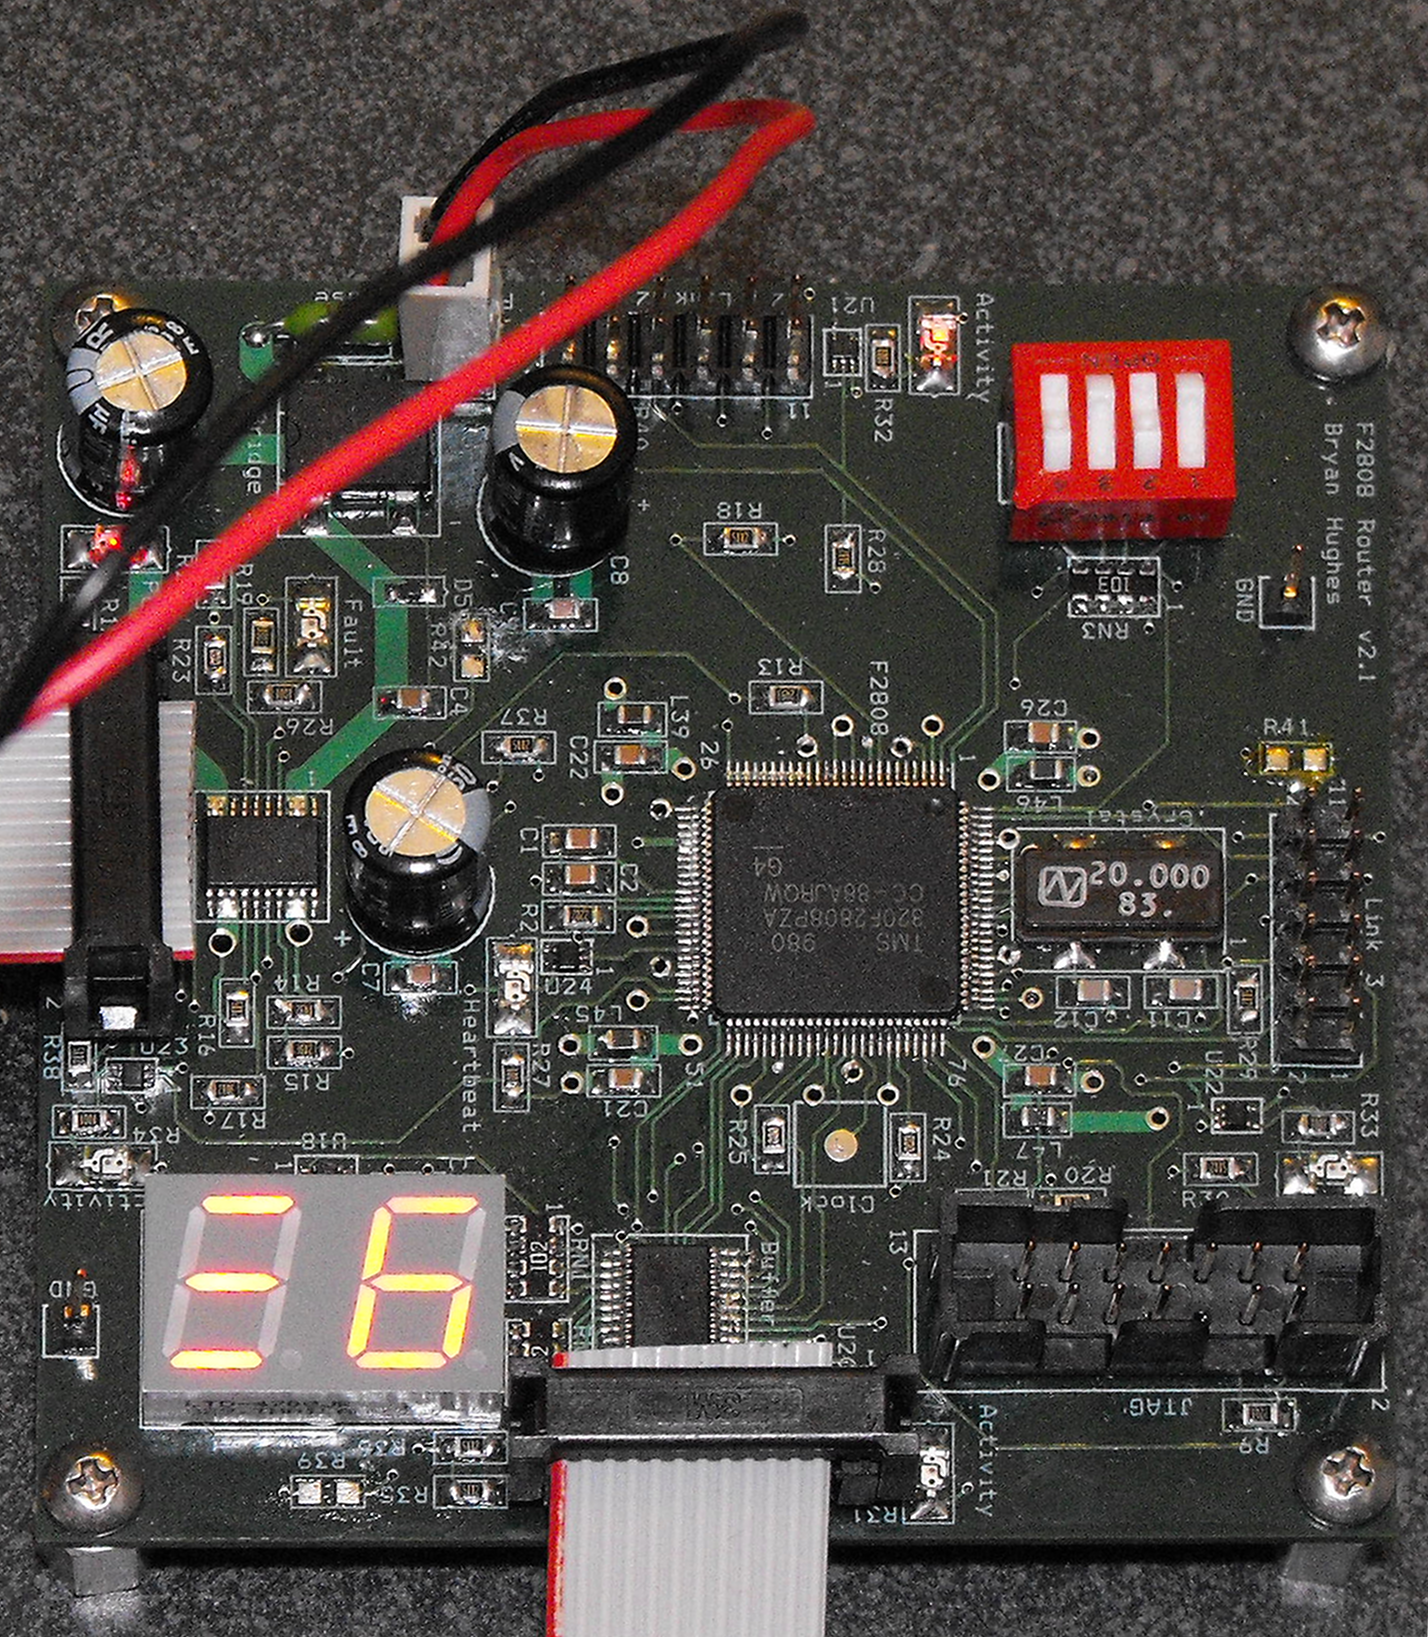
\includegraphics[width=6in]{Hardware/Figures/hardware-board_running.png}
		\caption{Prototyping Board Running}
		\label{fig:hardware:board_running}
	\end{centering}
\end{figure}

\section{Future Work}\label{sec:hardware:future_work}

The boards are pretty complete, but a few odds and ends could use improvement. As mentioned earlier, the latest board revisions still had a few errors to be corrected. In the future, these changes should be incorporated into the board design itself instead of relying on post-production modifications. Chances to the link header, described in Chapter \ref{sec:spi}, will also require updates to the board design. Configuring the Analog to Digital Converter (ADC) on these boards with a header for connecting devices could be useful for future work on distributed I/O, as would setting up a header for connecting external devices directly to the extra GPIO pins in the link header that were not used. The testing process for the later chapters has revealed that a reset switch on each board would have also been useful.

\section{Conclusions}\label{sec:hardware:conclusions}

In this chapter, a network prototyping board was presented that allows rapid prototyping of different network topologies. Each prototyping board consists of an F2808 DSC, a JTAG connector, a Seven Segment Display, DIP switches for run-time configuration, four peer-to-peer SPI links, and onboard power circuitry for protection and regulation. The board has been tested and verified to be fully functional with the final firmware. 



\chapter{Physical and Data Link Layer:\\ Peer-to-Peer Serial Peripheral Interface}\label{sec:spi}

\section{Background}\label{sec:spi:background}

The Serial Peripheral Interface (SPI) de-facto standard is a communications protocol that is supported by almost every microcontroller in the market and a number of other embedded devices. One of the first devices to incorporate SPI was the Motorola MC68HC05C4, which was also the first device to use the name ``SPI.'' \cite{ref:1994-motorola-spi} SPI is also called ``Microwire'' in some cases, especially on older National Semiconductor devices. \cite{ref:1995-national_semiconductor-microwire}

\subsection{The SPI ``Specification''}\label{sec:spi:background:spi_specification}

SPI is a master-slave, synchronous serial communications protocol that uses either three or four wires, depending on the configuration, and typically transmits up to one fourth of the clock speed of the device. SPI is considered a ``de-facto'' standard because, although no formal specification for SPI exists, manufacturers follow the same basic protocol. A number of variations between manufacturers and chips exist, however. Unless otherwise noted, this document is referring to the typical implementation of SPI. SPI is typically intended for point to point communications, although it can also be used in a bus configuration. 

A typical SPI interface in is shown in Figure \ref{fig:spi:typical_pinout}. The Master Out, Slave In (MOSI) pin is used to transfer data from a master device to a slave device, and the Master In, Slave Out (MISO, also called SOMI) transfers data from a slave to a master. The Clock (CLK) pin clocks data on these two lines. In typical three wire implementations, MOSI, MISO, and CLK are the three pins used.

\begin{figure}[ptb]
	\begin{centering}
		\includegraphics{SPI/Figures/spi-typical_pinout.pdf}
		\caption{Typical SPI Pinout}
		\label{fig:spi:typical_pinout}
	\end{centering}
\end{figure}

The fourth pin is the Slave Transmit Enable (STE) pin, and is where most variances between implementations occur. Typically, when asserted, the STE pin allows a slave to transmit to and receive from the master. The STE pin can be asserted high or low depending on the implementation. A variety of other configurations exist, so care must be taken to ensure that the STE pin behaves properly. For example, on the MSP430 microcontroller from Texas Instruments, the STE pin is also used to allow multiple masters on a single bus by suppressing communication from other masters, in addition to enabling slave communication \cite{ref:2009-ti-msp430}. The STE pin can also be used to allow bussed SPI transmissions. The master asserts the STE pin on the specific slave with which it wants to communicate while leaving the STE pins on the other devices de-asserted.

Typically, four clocking schemes are available to be configured. Data can be transmitted on the falling edge of the clock and received on the rising edge of the clock, or vice versa. By reading on the opposite edge of the write, the signal will have had time to settle, thus eliminating errors that would otherwise occur by reading while the signal is changing. Data can also be delayed by a half clock cycle to further increase stability. These four schemes are shown in Figure \ref{fig:spi:clocking_schemes}. Note that the master always generates the clock signal. This implies that the master must send a clock signal in order for the slave to transmit. The clock signal is generated whenever the master is transmitting, but what happens when the master has nothing to send but wants to give the slave a chance to transmit? It is customary to transmit dummy data consisting of all 0's to the slave.

\begin{figure}[ptb]
	\begin{centering}
		\subfigure[Transmit on Rising Edge, No Delay]
    {
			\includegraphics[width=6in]{SPI/Figures/spi-clocking_schemes_rise_no_delay.pdf}
			\label{fig:spi:clocking_schemes_rise_no_delay}
		}
		\subfigure[Transmit on Rising Edge, Half-cycle Delay]
    {
			\includegraphics[width=6in]{SPI/Figures/spi-clocking_schemes_rise_delay.pdf}
			\label{fig:spi:clocking_schemes_rise_delay}
		}
		\captcont{SPI Clocking Schemes}
		\label{fig:spi:clocking_schemes}
	\end{centering}
\end{figure}

\begin{figure}[ptb]
	\begin{centering}
		\subfigure[Transmit on Falling Edge, No Delay]
    {
			\includegraphics[width=6in]{SPI/Figures/spi-clocking_schemes_fall_no_delay.pdf}
			\label{fig:spi:clocking_schemes_fall_no_delay}
		}
		\subfigure[Transmit on Falling Edge, Half-cycle Delay]
    {
			\includegraphics[width=6in]{SPI/Figures/spi-clocking_schemes_fall_delay.pdf}
			\label{fig:spi:clocking_schemes_fall_delay}
		}
		\caption{SPI Clocking Schemes cont.}
		\label{fig:spi:clocking_schemes-continue_1}
	\end{centering}
\end{figure}

\subsection{Comparison with other embedded communication protocols}\label{sec:spi:background:comparison}

Two other communication protocols are commonly found on microprocessors that are used for inter-processor communication: Inter-Integrated Circuit (), and Controller Area Network Bus (CAN-Bus).

$\textrm{I}^2 \textrm{C}$ was originally developed by Philips for use by microcontrollers in TV sets. $\textrm{I}^2 \textrm{C}$ is commonly used to connect peripheral devices such as sensors, memory, and multimedia hardware codecs to a central microcontroller. $\textrm{I}^2 \textrm{C}$ is a bus-based protocol that uses two signals: serial clock and serial data. The master controls the clock, as in SPI, to prevent devices from communicating over each other. Unlike SPI, $\textrm{I}^2 \textrm{C}$ uses a primitive packet system. Devices come with a hardwired address, with the lower bits being user-configurable. Devices only respond to a message if a packet contains the correct device address. A simple Acknowledgement (ACK) system is included in the packet protocol. Devices can communicate at three different speeds: standard devices can communicate up to 100 kbps, fast-mode devices can communicate up to 400 kbps, and high-speed-mode devices can communicate up to 3.4 Mbps. \cite{ref:2001-embedded.com-i2c} 

Because $\textrm{I}^2 \textrm{C}$ is a bussed system, the communication speed is the aggregate speed for all devices. If every controller wants to communicate at the same time, the total bandwidth in an  node system available to a fast-mode device is $\frac{400 kbps}{n - 1}$, which is considerably slower than SPI. Even in the best-case scenario of $n=2$, SPI can still run faster on devices with clock speeds in the hundreds of megahertz. Another disadvantage of bus-based systems is that the maximum size of the network is limited to a handful of nodes for all practical purposes. One advantage of $\textrm{I}^2 \textrm{C}$ is that it is an official standard, so different implementations will ``just work,'' whereas SPI can take some additional hardware to properly interface different implementations.

CAN-bus is another bus-based system that was originally developed by Bosch, an automotive parts manufacturer, as a solution to cable management problems in automobiles with a large number of microcontrollers and sensors. CAN-bus uses a two-wire differential interface carrying the data signal that can operate up to 1 Mbps. CAN-bus optionally includes ground and power lines, which allows fault-tolerance if one of the data lines is severed. CAN-bus is a peer-to-peer network that uses a clever arbitration system. The outputs of all nodes form a wired-OR network, and nodes read back everything they write to the bus to see if anyone else is also transmitting. By the time the header has been transmitted, the system has arbitrated itself without requiring re-transmission from the node that won the arbitration. CAN-bus uses a packet system that includes error detection, ACK capabilities and a data payload of 8 bytes. A few protocols are designed to run on top of CAN-bus, which further simplifies messaging. \cite{ref:2003-embedded.com-canbus}

Can-bus also suffers from the same performance issues as $\textrm{I}^2 \textrm{C}$ because it is bussed, while SPI does not suffer such issues. CAN-bus does provide a lower barrier of entry, especially when paired with a higher-level protocol, because less must be done to support messaging between nodes. CAN-bus is also a true peer-to-peer system, which is advantageous in distributed systems, as will become evident in Section \ref{sec:spi:background:distributed_systems}.

\subsection{Distributed Systems Using SPI} \label{sec:spi:background:distributed_systems}

Before SPI can be used effectively as the underlying protocol for a distributed system, one concern must be addressed: SPI is a master/slave protocol. While it is possible to realize a distributed system with SPI's master/slave system, it would be extremely difficult. For example, if three nodes are connected to each other in a ring, then which nodes should be masters and which nodes should be slaves? There isn't a solution in this case, and there are many other topologies that can't be realized in a master/slave situation if the node is configured fully as a master or fully as a slave. Mixed configurations, a.k.a. one port is a master and the other is a slave, can solve this problem, but it adds complexity for the end-user. In the topologies that can be implemented with a master/slave system, the issue remains of configuring each node manually to be a master or a slave. The other problem is one of utilization. In order for a slave to transmit, the master must also transmit, which can be inefficient because the master does not know when the slave wants to transmit. If the master does not transmit all the time, then a delay is incurred when the slave wants to transmit but must wait for the master to transmit. One solution to this problem is for the master to transmit dummy data all the time, but aside from inelegance, the problem of determining which data is dummy data and which data is valid data must be solved. These are solvable problems, but they require more complex code and overhead. A peer-to-peer system is the preferred method to provide a true plug-and-play system that is easy for the user to implement and is efficient. 

\section{Objectives}\label{sec:spi:objectives}

As mentioned in Chapter \ref{sec:introduction}, the physical and data link layer must meet the following criteria: 
\begin{enumerate}
	\item Scalable
	\item Available on a wide variety of devices
	\item Peer-to-peer
\end{enumerate}

\section{Methodology}\label{sec:spi:methodology}

As discussed in Section \ref{sec:spi:background:comparison}, bussed systems are not scalable and do not satisfy the scalability objective. SPI is a suitable choice for use in a distributed system with multiple processors, as long as it is used as a point-to-point protocol and not as a bussed protocol, which satisfies the first two objectives. An example of the suitability of SPI to distributed systems can be found in \cite{ref:2007-szekacs-multiprocessor_spi_system}, where the authors began their project using $\textrm{I}^2 \textrm{C}$  but soon ran into limitations and expanded it using SPI.

In order to satisfy the third objective, the question becomes: how does one change SPI into a peer-to-peer protocol? Looking back at figure \ref{fig:spi:typical_pinout}, notice that the same lines are used for both slave and master configurations, and that the only difference between a master and a slave is the software configuration. This makes it possible to switch a device from a slave to a master and back dynamically. Changing a processor from a slave to a master and back forms the crux of the proposed solution.

In the solution, every device is configured as a slave by default. Whenever a device must communicate with a neighbor, it temporarily changes \emph{only the port connected to the neighbor} to a master. This gives a proper master/slave configuration on that port, while allowing the other ports to arbitrate to whatever configuration is required for that link. This process is called ``port elevation.'' Once elevated, the node transmits one flit\footnote{A flit is the basic unit of data in a transmission, similar to a Minimum Addressable Data Unit (MADU) in memory} of data. When the transmission is complete, the node reverts back to a slave, called ``port demotion.'' Two problems exist with this mechanism. The first problem is that this reduces SPI to a half-duplex transmission mechanism, but this issue is deemed as an acceptable loss because the bandwidth left is still much greater than that of the other mechanisms. The second problem is that no mechanisms are in place to prevent transmission collisions.

To prevent collisions, an arbitration scheme has been developed that uses the MISO pin as a GPIO pin, called the Master Arbitrate (MARB) pin. This connection is illustrated in Figure \ref{fig:spi:p2p_pinout}. The arbitration process is shown in Figure \ref{fig:spi:arbitration_scheme} and guarantees that a node will not transmit over another node. The arbitration scheme works by first checking the MARB line to see if another node is transmitting. If not, then the port attempts to claim the line by asserting MARB. Two nodes could attempt to talk at the exact same time, which would go unnoticed, so the node then waits for a pre-determined period of time that is different than the other node, and then checks the MARB line again to see if the other node has attempted to elevate. This mechanism guarantees against collisions because each node is forced to wait a different amount of time before checking again. The wait time is assigned based on the port number, which guarantees different wait times as long as the same two port numbers are not connected.

\begin{figure}[ptb]
	\begin{centering}
		\includegraphics{SPI/Figures/spi-p2p_pinout.pdf}
		\caption{Pin-out for Peer-to-Peer based SPI}
		\label{fig:spi:p2p_pinout}
	\end{centering}
\end{figure}

\begin{figure}[ptb]
	\begin{centering}
		\includegraphics{SPI/Figures/spi-arbitration_scheme.pdf}
		\caption{Arbitration Scheme}
		\label{fig:spi:arbitration_scheme}
	\end{centering}
\end{figure}

To improve performance of the system, virtual channels are employed. A virtual channel is a logical channel that resides on top of a physical channel. Multiple virtual channels can be used on a single physical channel as long as each flit has a means of identifying the virtual channel on which it resides. Using multiple virtual channels allows the transmitter to interleave flits from different packets, which improves performance. In systems that do not use virtual channels, a large packet sent across a physical channel prevents smaller packets from using that channel, which increases latency and can potentially cause buffer overflows. If virtual channels are implemented, however, the smaller packets can be sent in parallel with the large packet, which eliminates that bottleneck.\footnote{For more information on Virtual Channels, read chapter 2 section 4 of \cite{ref:1997-duato-interconnection_networks}}
Determining how many virtual channels to use is very important, especially if the base flit size is small. If too few virtual channels are used, then channels can still become blocked by transmissions. If too many virtual channels are used, then the overhead necessary to identify which virtual channel a flit is on can become proportional to the flit itself. Through experimentation, 16 virtual channels (4 bits of overhead) are enough to eliminate bottlenecks the majority of the time while keeping overhead low in this application. 
Each flit is 144 bits long. 128 bits are reserved for the network layer, and the remaining 16 bits are used for the Data Link Layer, shown in Figure \ref{fig:spi:data_link_header}. The header contains the destination address of the flit, the virtual channel on which the flit is being transmitted, and the flit type. The destination address isn't really a data link layer function, and is more or less included as padding to make the flit size a multiple of 16 and to make obtaining the destination address during processing easier. The flit type field is used to identify which of the possible flit types, shown in Table \ref{tab:spi:flit_types}, this flit is. The flit type lets the network-level protocol stack know what to do with the flit. The virtual channel field indicates the virtual channel on which this flit is being transmitted. Virtual channel 0 is reserved for system use, virtual channels 1-14 are for data transfers, and virtual channel 15 is for network-level packet headers. Headers are given a dedicated virtual channel because a) headers occupy a single flit and thus don't require virtual channels to be reserved and b) a dedicated channel ensures that packet headers can always flow through the system unimpeded.

\begin{figure}[ptb]
	\begin{centering}
		\includegraphics{SPI/Figures/spi-data_link_header.pdf}
		\caption{Data Link Layer Header}
		\label{fig:spi:data_link_header}
	\end{centering}
\end{figure}

\begin{table}
	\begin{center}
	\setlength{\extrarowheight}{1.5pt}
		\caption{List of Flit Types}
		\vspace{0.1cm}
		\begin{tabular}{|l|l|}
			\hline
			\textbf{Flit Type} & \textbf{Description}	\\
			\hline
			\hline
			Header	& A protocol-level header packet \\
			\hline
	       Payload	& Part of a protocol-level data payload \\
			\hline
	       End of payload	& Last flit in a protocol-level data payload \\
			\hline
		\end{tabular}
		\label{tab:spi:flit_types}
	\end{center}
\end{table}

In traditional implementations, each virtual channel gets its own receive and transmit buffers. If buffer capacity can be easily extended to provide each virtual channel with the same buffer capacity that a single physical channel would otherwise have, then this configuration is no problem. However, this method isn't feasible in systems with limited memory. In order to give each virtual channel its own buffer in this environment means shrinking the size of the buffers. Instead, a more efficient approach is used whereby a single receive buffer is shared by all virtual channels across all ports, and one shared transmit buffer is shared by all virtual channels for each port. Buffers are shared across virtual channels because only some of the virtual channels will be used at any specific point of time. If buffers were not shared, then the input buffer for one virtual channel could overflow, while the others remained empty. A single input buffer is used across all ports because the port which a flit arrives usually has little, if any, impact on where it is going.

\section{Implementation}\label{sec:spi:implementation}

The software implementation for the physical and data link layers are divided into three groups: buffer management, transmission, and reception.

\subsection{Buffer Management Functions}\label{sec:spi:implementation:buffer_management_functions}

Three functions are used to enqueue and dequeue flits from the buffers: \lstinline$EnqueInboundFlit()$, \lstinline$DequeInboundFlit()$, and \lstinline$EnqueOutboundFlit()$. Dequeueing of outbound flits is handled directly by the transmission software for performance reasons, and thus there is no separate function for it. The buffers are implemented as circular buffers; they are declared as static arrays and a pointer to the head and tail of the queue keeps track of the queue. This makes it very efficient to enqueue/dequeue an item because other items do not need to be shifted around after an item is added/removed. 

Each buffer has a control function associated with it that runs in its own thread. \lstinline$ProcessInboundFlits()$, described in Section \ref{sec:spi:implementation:reception}, dequeues flits from the receive buffer and processes them. \lstinline$ProcessOutboundFlits()$, described in Section \ref{sec:spi:implementation:transmission}, dequeues flits from the transmit buffer and transmits them on the appropriate port. These threads and their relationships to the buffers are illustrated in Figure \ref{fig:spi:software_architecture}. These functions drive the rest of the system in a data-driven manner.

\begin{landscape}
	\begin{figure}[ptb]
		\begin{centering}
			\includegraphics[width=8.5in]{SPI/Figures/spi-software_architecture.pdf}
			\caption{Software architecture of SPI systems}
			\label{fig:spi:software_architecture}
		\end{centering}
	\end{figure}
\end{landscape}

\subsection{SPI Transmission}\label{sec:spi:implementation:transmission}

Each port is configured to run at 20 MHz because the time spent in this function must be minimized, and this speed was experimentally found to be the fastest reliable speed which the F2808 can run. The SPI is configured to use 16-bit words. It makes sense to configure the SPI FIFOs to contain a single flit, so the receive FIFO is configured to interrupt when 9 words (144 bits) have been received. The SPI is configured to transmit on the falling edge of the clock, without a delay. This configuration was chosen because it is the most common configuration among SPI devices.

There is a single transmission function: \lstinline$ProcessOutboundFlits()$. This code is extremely sensitive to timing, and so interrupts are disabled when this function is running. In addition, this thread has the highest priority of all running threads, which prevents any other threads from running. To prevent the rest of the system from being locked, this function must be as efficient as possible. The function is implemented as a state diagram with five possible states plus an error state. This function must manage all ports on the device simultaneously, and many of these states require a delay between them. Using states allows the function to interleave the transmission for each port. The code works by checking whether each port is in a given state in the order shown in Figure \ref{fig:spi:transmit_state_charts}, and if so, executes according to the associated flow-chart. This has the effect of causing the ports to run in ``lock-step'' with each other in most cases, although each port does have the freedom to diverge in the case of arbitration issues. 

\begin{landscape}
	\begin{figure}[p]
		\begin{centering}
			\includegraphics[width=8.5in]{SPI/Figures/spi-transmit_state_charts.pdf}
			\caption{Flowchart of States for \lstinline$ProcessOutboundFlits()$}
			\label{fig:spi:transmit_state_charts}
		\end{centering}
	\end{figure}
\end{landscape}

One interesting side-effect of the port elevation and demotion was uncovered during the development process: all of the internal logic on the F2808 is hardwired for input or output, regardless of whether or not the port is a master or slave. The upshot of is that the interrupt logic for the receiver in slave mode becomes the interrupt logic for the transmitter in master mode. As a result, this caused the F2808 to trigger a receive interrupt after a port was demoted and thus called the receiver interrupt routine, even though no data had actually been received! The solution is to reset all interrupts after the port has finished transmitting but before the port is demoted, and the interrupt is squashed before it reaches the PIE.

\subsection{SPI Reception}\label{sec:spi:implementation:reception}

SPI reception is composed of two primary parts: the SPI interrupt and the \lstinline$ProcessInboundFlits()$ function. The interrupt routine dequeues the flit out of the SPI FIFO, enqueues the flit in the inbound flits queue, and wakes up the \lstinline$ProcessInboundFlits()$ function if need be. The \lstinline$ProcessInboundFlits()$ function first dequeues the oldest flit in the inbound flits queue. If the flit is a header flit, it is sent on to be processed by the network-level protocol stack, described in Chapter \ref{sec:protocol}. If the flit is a data payload flit, then it directly enqueued into the appropriate outbound flit queue. If the flit is the end of a data payload, it is enqueued into the appropriate outbound flit queue, and the stored transmission information is finalized. Note that the protocol stack handles setting up the transmission information. Moving the major flit processing out of the interrupt routine and into a separate thread keeps the interrupt routine really short and prevents it from blocking other threads for too long. In the event that the receive buffer is full after a flit has been enqueued, then all MARB pins are asserted as a flow control mechanism to prevent any other nodes from transmitting until a flit is dequeued from the buffer.

\section{Results}\label{sec:spi:results}

To ensure that the links behaved as expected, the lines were inspected electrically to examine the waveforms. Figure \ref{fig:spi:link_waveform} shows the relevant signals for a single link. Figure \ref{fig:spi:waveform_comparison} shows the MARB signals across the four links. Note that when the MARB signal goes low, it is checking the other signal to see if there was a collision. There is no possibility of missing a collision because each link checks at a different time, unless the same links are connected together, which is an easily avoidable configuration.

\begin{landscape}
	\begin{figure}[p]
		\begin{centering}
			\includegraphics[width=8.5in]{SPI/Figures/spi-link_waveform.png}
			\caption{Link waveform}
			\label{fig:spi:link_waveform}
		\end{centering}
	\end{figure}
\end{landscape}

\begin{landscape}
	\begin{figure}[p]
		\begin{centering}
			\includegraphics[width=8.5in]{SPI/Figures/spi-waveform_comparison.png}
			\caption{Comparison of arbitration waveforms across all links}
			\label{fig:spi:waveform_comparison}
		\end{centering}
	\end{figure}
\end{landscape}

The code has been tested extensively to ensure correctness. A test has been devised that uses custom code that doesn't contain any non-essential code. While this test is not a real-world scenario, it allows individual sections of code to be tested much more rigorously because the processor won't be spending time running non-essential pieces of code. The test has two nodes continuously transfer known dummy data to each other, and the received flits are checked on the other side for correctness. Each node keeps track of how many flits it sent, how many flits it correctly received, and how many flits were received with errors. This test stresses the arbitration scheme because both nodes are trying to transmit over the same link continuously. The results for each node are shown in Table \ref{tab:spi:endurance_test}. As one can see, the system is perfect at the SPI level. No collisions were tested in this case scenario, unfortunately, because the time window available for a collision to occur is only two to three clock cycles. A few undocumented cases were observed during later testing where collisions were detected and successfully avoided. If a collision is not detected properly, then the flit will simply go missing because the ``receiving'' node is not listening for the exact amount of time that the transmission is occurring. No message garbling occurs.

\begin{table}
	\begin{centering}
		\setlength{\extrarowheight}{1.5pt}
		\caption{SPI Endurance Test}
		\vspace{0.1cm}
		\begin{tabular}{|c|c|c|c|}
			\hline
			\textbf{Node} &	\textbf{Flits Sent} & \textbf{Flits Correctly Received} & \textbf{Flits Incorrectly Received} \\
			\hline
			\hline
	       1 & 500000 & 500000 & 0 \\
	       \hline
	       2 & 500000 & 500000 & 0 \\
	       \hline
		\end{tabular}
		\label{tab:spi:endurance_test}
	\end{centering}
\end{table}
		
\section{Future Work}\label{sec:spi:future_work}

The arbitration scheme discussed here was created rather late in the project. The original scheme called for two arbitration lines that were always owned by a node, regardless of whether or not the port was elevated. This mechanism utilized the STE pin for one of the arbitration lines because it was believed at the time that STE was unnecessary for the prototype hardware, which turned out to be incorrect. A future improvement would be to add the second arbitration pin back to the header link. While the current scheme does guarantee against collisions, it also doubles the amount of time necessary to transmit a flit. The other two-pin arbitration scheme is much faster because it does not need to check the arbitration line twice. Another potential improvement would be to allow link ``ganging,'' i.e. multiple links can be used between two nodes to increase bandwidth. It is also possible to transmit multiple flits together so that a node only  arbitrates once for all of the flits, instead of once per flit. This has the advantage of reducing arbitration overhead, but care would need to be taken to ensure that one node doesn't monopolize the link.

\section{Conclusions}\label{sec:spi:conclusions}

In this chapter, a peer-to-peer variant of SPI was presented that serves as the Physical and Data Link Layers in the prototype toolkit. At the physical layer, an arbitration scheme has been developed that uses an extra GPIO pin for arbitration to prevent collisions, and has been tested thoroughly. At the data link layer, virtual channels have been employed to reduce congestion in the network. Careful attention has been paid to maximizing the effectiveness of buffers on the memory-limited F2808 DSC. This mechanism has shown good robustness and serves as a foundation for the rest of the toolkit.
\chapter{Network Layer:\\ A Custom Embedded-Oriented Protocol}\label{sec:protocol}

\section{Background}\label{sec:protocol:background}

A variety of protocols exist that are geared toward different types of networks. Section \ref{sec:protocol:background:switching} will consider a variety of switching techniques. Section \ref{sec:protocol:background:protocols} will consider two popular protocols currently in widespread use: the Internet Protocol Suite, also known as Transmission Control Protocol and Internet Protocol (TCP/IP) over Ethernet, and RapidIO. Switching is discussed first because the switching techniques employed in a given protocol generally influence the information that a protocol includes in its packet headers. Finally, communication faults are discussed in Section \ref{sec:protocol:introduction:communication_faults}.

\subsection{Overview of Select Existing Switching Mechanisms}\label{sec:protocol:background:switching}

Switching techniques determines how a data packet is forwarded through a network. Switching is not to be confused with routing, which determines \emph{where} a data packet is sent in the network. The switching technique determines if and how links are reserved, the relationship between the header and the data payload as they travel through the network, etc. Many different types of switching exist, so this section will focus on the following basic types of switching: virtual circuit switching, packet switching, virtual cut-through switching, wormhole switching, and pipelined circuit switching.
Circuit switching was originally developed for the Plain Old Telephone System (POTS) and is called circuit switching because the early automated switching devices used electro-mechanical circuits configured in an array to connect one end to the other. Circuit switching in modern information networks (called Virtual Circuit Switching) uses completely different hardware, of course, but many of the basic principles still apply. The main differentiating characteristic of circuit switching is that a network path is reserved \emph{prior} to sending any data. The path is typically reserved by first sending a ``probe'' packet. This packet is sent to the destination, and each node the probe passes through reserves the appropriate links. When the entire path is reserved, the destination sends an acknowledgement back to the sender indicating that data transmission can commence. The data packet is then transferred along the reserved path. The time-space diagram of a packet being sent through a virtual circuit switching network is shown in Figure \ref{fig:protocol:vcs_time_diagram}. In the figure, $t_r$ is the processing time spent making routing decisions and $t_s$ is the processing time spent making switching decisions. The primary advantages of circuit switching are that it is simple to implement and that it is very reliable after a path is established. The primary downside to circuit switching is that after a path is reserved, no other transfers can use those links, which can increase congestion. Circuit switching is advantageous in networks where packets are infrequent and long. \cite{ref:1997-duato-interconnection_networks}

\begin{figure}[ptb]
	\begin{centering}
		\includegraphics[scale=0.8]{Protocol/Figures/protocol-vcs_time_diagram.pdf}
		\caption[Virtual Circuit Switching Time Diagram]{Virtual Circuit Switching Time Diagram \cite{ref:1997-duato-interconnection_networks}}
		\label{fig:protocol:vcs_time_diagram}
	\end{centering}
\end{figure}

Packet switching does not reserve a channel prior to transmitting and instead transmits the data payload with the packet header. Packet switching works best with small packet sizes, so large messages are typically broken into multiple smaller packets. Each packet contains its own header and is routed independently of the other packets to the destination. Every packet is fully buffered at each node $x$, and then forwarded to the next node. This mechanism makes packet switching very robust to congestion, but at the expensive of more overhead in the packet headers and in processing at each node. In particular, packet switching requires large amounts of buffer storage at each node so it can potentially buffer several complete packets at a time, which is something that is often not possible in embedded processors. The time-space diagram is shown in Figure \ref{fig:protocol:ps_time_diagram}. Packet switching is advantageous in networks where packets are frequent and short. \cite{ref:1997-duato-interconnection_networks}

\begin{figure}[ptb]
	\begin{centering}
		\includegraphics[scale=0.8]{Protocol/Figures/protocol-ps_time_diagram.pdf}
		\caption[Packet Switching Time Diagram]{Packet Switching Time Diagram \cite{ref:1997-duato-interconnection_networks}}
		\label{fig:protocol:ps_time_diagram}
	\end{centering}
\end{figure}

Virtual cut-through switching is a modified version of packet switching that takes advantage of the fact that packet headers occur at the beginning of a packet. This mechanism allows a node to inspect the header as soon as it has arrived and to determine what to do with the packet. The node then begins forwarding data as soon as it arrives. In the case of a blocked path, the entire message is buffered at the node. This eliminates the need for large data buffers in the network because flits can be forwarded as soon as they arrive, and it is reasonable to assume that there won't be a ``pile-up'' of blocked messages. The time-space diagram is shown in Figure \ref{fig:protocol:vcts_time_diagram}. Virtual cut-through switching does decrease latency and buffer capacity, but still suffers from high complexity. \cite{ref:1997-duato-interconnection_networks}

\begin{figure}[ptb]
	\begin{centering}
		\includegraphics[scale=0.8]{Protocol/Figures/protocol-vcts_time_diagram.pdf}
		\caption[Virtual Cut-Through Switching Time Diagram]{Virtual Cut-Through Switching Time Diagram \cite{ref:1997-duato-interconnection_networks}}
		\label{fig:protocol:vcts_time_diagram}
	\end{centering}
\end{figure}

Wormhole switching is very similar to virtual cut-through switching in that it begins forwarding flits as soon as they are available. The key difference between virtual cut-through switching and wormhole switching is how they deal with blocked links. In wormhole switching, a blocked path results in the transmission ``stalling'' where it is. In other words, transmission stops where it is, leaving the packet spread across multiple routers. As a result, the complexity is higher than virtual cut-through switching, but it requires significantly smaller buffers compared to virtual cut-through switching. The time-space diagram for wormhole routing is shown in Figure \ref{fig:protocol:ws_time_diagram}. \cite{ref:1997-duato-interconnection_networks}

\begin{figure}[ptb]
	\begin{centering}
		\includegraphics[scale=0.8]{Protocol/Figures/protocol-ws_time_diagram.pdf}
		\caption[Wormhole Switching Time Diagram]{Wormhole Switching Time Diagram \cite{ref:1997-duato-interconnection_networks}}
		\label{fig:protocol:ws_time_diagram}
	\end{centering}
\end{figure}

Pipelined circuit switching is designed to make wormhole routing more fault tolerant, at the expense of performance. In wormhole routing, if the header gets stuck somewhere due to a faulty component or blocked link, the data payload stalls in the network, leaving the resources unavailable for other transfers. In pipelined circuit switching, instead of sending the data payload immediately after sending the header, the connection is first reserved using the same mechanisms as virtual circuit switching and then the data payload is sent. In order to prevent blocked messages, virtual channels, described in Chapter \ref{sec:spi}, are utilized. This method is called a ``hybrid'' switching technique because it combines elements of wormhole routing and virtual circuit routing. Pipelined circuit switching requires very small buffers, as in wormhole routing, but it also has the fault tolerance of virtual circuit routing and is very good at avoiding blocked links, while also being considerably simpler. The time-space diagram for pipelined circuit switching is shown in Figure \ref{fig:protocol:pcs_time_diagram}. \cite{ref:1997-duato-interconnection_networks}

\begin{figure}[ptb]
	\begin{centering}
		\includegraphics[scale=0.8]{Protocol/Figures/protocol-pcs_time_diagram.pdf}
		\caption[Pipelined Circuit Switching Time Diagram]{Pipelined Circuit Switching Time Diagram \cite{ref:1997-duato-interconnection_networks}}
		\label{fig:protocol:pcs_time_diagram}
	\end{centering}
\end{figure}

\subsection{Overview of Select Existing Protocols}\label{sec:protocol:background:protocols}

A variety of protocols exist that have been developed for different purposes. TCP/IP is ubiquitous in large scale networks and is the protocol used by personal computers and the Internet. Other protocols have been used in the past, such as NetBIOS over IPX/SPX, but have fallen out of favor in exchange for TCP/IP. Other protocols in use tend to be more special purposes than TCP/IP. PCI Express (PCIe), for example, is used to connect peripherals in a personal computer to the main processor. RapidIO has recently become popular in high-end embedded systems.

\subsubsection{TCP/IP Overview}\label{sec:protocol:background:protocols:tcpip}

TCP/IP is a suite of layered protocols that provide the primary protocols used for intranets and the Internet. The term TCP/IP is often used to denote different things depending on the context. For the purposes of this discussion, TCP/IP will refer to the protocols in the network and transport layers, but not in the data link/application/etc layers. TCP/IP is run on many different types of data link layers, but the most common is Ethernet. Ethernet is a shared medium physical and data link layer protocol and is analogous to the peer-to-peer mechanism described in Section \ref{sec:spi}.  Ethernet utilizes a 22 byte header, shown in Figure \ref{fig:protocol:ethernet_header}, which adds overhead to the system. The header is responsible for conditioning the signal, specifying source and destination hardware addresses, and specifying the data length. Ethernet switches typically use packet switching, although some variations exist. \cite{ref:2004-forouzan-data_communications_and_networking}

\begin{landscape}
	\begin{figure}[p]
		\begin{centering}
			\includegraphics{Protocol/Figures/protocol-ethernet_header.pdf}
			\caption[Ethernet Header]{Ethernet Header \cite{ref:2004-forouzan-data_communications_and_networking}}
			\label{fig:protocol:ethernet_header}
		\end{centering}
	\end{figure}
\end{landscape}

The most important TCP/IP protocol at the network layer is the IP protocol. This protocol handles data transmissions originating from the higher layers. The other protocols are generally management-oriented or extend the IP protocol. The current IP protocol, IPv4, has been around for almost 30 years and will soon be replaced by IPv6. Due to the prevalence of IPv4, however, this paper will only consider it. IPv4 accepts data from the transport layer, packages it into an IP packet, and sends it to the data link layer. In the context of the Internet, IPv4 is responsible for delivering the packet to the final destination. By itself, IPv4 uses universal addresses for all nodes. These IP addresses are assigned by central authorities, such as the Internet Corporation for Assigned Names and Numbers (ICANN). Technologies such as Network Address Translation (NAT) allow private IP addresses that are not universally unique. IPv4 does not specify how to route a packet, and IPv4 supports arbitrary data fragmentation. These features allow IPv4 to be used on different types of networks with different types of routing protocols and packet lengths. The IPv4 header is shown in Figure \ref{fig:protocol:ip_header}. The options field in the header is the only variable length field, and usually isn't used. When unused, the total header length is 20 bytes long. The source and destination specify the initial source and final destination of the transfer, respectively. There is also a header checksum, assortment of flags, packet ID, and other information.  The fragment offset specifies where a data fragment fits into the full packet. Note that this implies, interestingly enough, that the process of partitioning the data into fragments and reassembling them on the other side \emph{is not handled} by IP. \cite{ref:2005-kozierok-tcpip_guide}

\begin{landscape}
	\begin{figure}[p]
		\begin{centering}
			\includegraphics{Protocol/Figures/protocol-ip_header.pdf}
			\caption[IP Header]{IP Header \cite{ref:2005-kozierok-tcpip_guide}}
			\label{fig:protocol:ip_header}
		\end{centering}
	\end{figure}
\end{landscape}

Two protocols are commonly used at the transport layer in TCP/IP: the Transmission Control Protocol (TCP) and the User Datagram Protocol (UDP). TCP provides connection oriented transmission with guaranteed delivery and other services. TCP operations are generally divided into three phases: connection phase, data transfer phase, and termination phase. TCP uses a client/server model, with the server listening on a port. A client that wants to communicate with the server first establishes a connection with the server by talking on the port where the server is listening. After the client and server have finished handshaking, the client can start sending data to the server. After the client is finished sending data, the connection is closed by the client. The header for a TCP packet is shown in Figure \ref{fig:protocol:tcp_header}. The header specifies the source port on the client and the destination port on the server. The sequence number is used to reassemble the fragmented data in the correct order when the packets have been received. The sequence number also indicates that a data packet was not transmitted correctly when a gap in sequence numbers is detected. The acknowledgement number is used to ACK data transfers for guaranteed delivery. TCP allows multiple data packets to be sent before an ACK is required. The amount of data that can be sent before an ACK is required is specified in the window field. The window size can also be used for flow control by setting it to 0. \cite{ref:2005-kozierok-tcpip_guide}

\begin{landscape}
	\begin{figure}[p]
		\begin{centering}
			\includegraphics{Protocol/Figures/protocol-tcp_header.pdf}
			\caption[TCP Header]{TCP Header \cite{ref:2005-kozierok-tcpip_guide}}
			\label{fig:protocol:tcp_header}
		\end{centering}
	\end{figure}
\end{landscape}

UDP provides a much more basic (and efficient) connectionless transmission without guaranteed delivery. UDP provides the minimum necessary functionality for a transport level protocol. The maximum length of a UDP packet is, in practice, determined by the underlying network layer, which is 65,507 bytes for IPv4. Because IPv4 does not guarantee delivery, packets can arrive out of order or may not arrive at all, and it is the responsibility of the programmer to handle these situations. The header, shown in Figure \ref{fig:protocol:udp_header}, is 8 bytes long. The short header size, combined with the lack of handshaking/etc. means that UDP has considerably less overhead than TCP, and is ideal for scenarios where some data loss is tolerable, such as streaming media. \cite{ref:2005-kozierok-tcpip_guide}

\begin{landscape}
	\begin{figure}[ptb]
		\begin{centering}
			\includegraphics{Protocol/Figures/protocol-udp_header.pdf}
			\caption{UDP Header \cite{ref:2005-kozierok-tcpip_guide}}
			\label{fig:protocol:udp_header}
		\end{centering}
	\end{figure}
\end{landscape}

\subsubsection{RapidIO Overview}\label{sec:protocol:background:protocols:rapidio}

RapidIO was developed specifically for high-end embedded systems and provides physical, data link, and network level communications. RapidIO is a chip-to-chip and board-to-board level interconnect and runs at speeds up to 10 Gbps. RapidIO was designed with the following set of objectives in mind \cite{ref:2005-fuller-rapidio_the_embedded_interconnect}:
\begin{enumerate}
	\item Focus on devices that are ``within the chassis'', i.e. connecting devices in the same system
	\item Limit the impact on software, i.e. do as much in hardware as possible
	\item Confine the protocol overhead so it is as small as possible
	\item Partition the specification into layers
	\item Manage errors in hardware
	\item Limit the silicon footprint
	\item Leverage established I/O driver/receiver technology, i.e. should be implementable in CMOS so that external physical layer hardware is unnecessary
\end{enumerate}
Services are defined at three layers: physical, transport and logical layers. The physical layer defines both a parallel and a serial implementation, handles flow control, low-level error detection/correction, basic packet information, and other services traditionally defined in the data link layer. The transport layer defines the network layer information, including addressing schemes and routing. The logical layer defines several APIs and mechanisms that clients use to communicate. \cite{ref:2005-fuller-rapidio_the_embedded_interconnect}
The serial physical layer uses 8B/10B encoding and supports either one differential pair or four differential pairs (called lanes) that are ``ganged'' together. Data can be transmitted at 1, 2, or 2.5 Gbps per lane. A 3 byte packet header is defined for the serial physical layer and includes ACK and CRC information. The parallel physical layer uses 8- or 16-bit wide LVDS lanes and operates at frequencies of 250 MHz to 1 GHz. The parallel packet is slightly different than the serial variant in specification but contains the same information. The physical layer defines several control packets used for port initialization, error recovery, and flow control for both implementations. \cite{ref:2005-fuller-rapidio_the_embedded_interconnect}
The transport layer is independent of the physical layer and routing implementation. The transport layer header defines three common fields: \emph{Source Address}, \emph{Destination Address}, and \emph{TT} (Transport Type). The 2-bit \emph{TT} field defines the type of transport packet and the other header fields that are included. Currently, \emph{TT}=00 defines 8-bit device IDs, \emph{TT}=01 defines 16-bit device IDs, and \emph{TT}=1x is undefined. The transport layer can optionally add other fields, such as a \emph{Hop Count} field or other management fields. The transport header and logical header are ``interleaved'' in the sense that they are not encapsulated, but rather have their fields defined in a single common specification, as shown in Figure \ref{fig:protocol:rapidio_packets}. This also implies that the logical APIs \emph{must} be used. \cite{ref:2005-fuller-rapidio_the_embedded_interconnect}
The logical layer mechanisms are all defined using a transaction model; communication is always performed in a request-response manner. Request and response packets each have their own basic header definition, with further fields being defined based on the transaction type. The transaction types are grouped according to function into the following groups: I/O, message passing, distributed shared memory, and data streaming. Other protocols, such as PCI, can be transported over RapidIO. When all three layers are taken together, packet overhead can range from 16 to 20 bytes. Typical request and response packets are shown in Figures \ref{fig:protocol:rapidio_packets:request} and \ref{fig:protocol:rapidio_packets:response}, respectively. \cite{ref:2005-fuller-rapidio_the_embedded_interconnect}

\begin{landscape}
	\begin{figure}[ptb]
		\begin{centering}
			\subfigure[Request Packet]
			{
				\includegraphics[scale=0.9]{Protocol/Figures/protocol-rapidio_request_header.pdf}
				\label{fig:protocol:rapidio_packets:request}
			}
			\subfigure[Response Packet]
			{
				\includegraphics[scale=0.9]{Protocol/Figures/protocol-rapidio_response_header.pdf}
				\label{fig:protocol:rapidio_packets:response}
			}
			\caption{Typical RapidIO request and response packets}
			\label{fig:protocol:rapidio_packets}
		\end{centering}
	\end{figure}
\end{landscape}

\subsection{Communication Faults}\label{sec:protocol:introduction:communication_faults}

Four primary faults can occur at the network layer: dead-lock, live-lock, starvation, and path cycles. These faults can cause a communication system to become completely unresponsive and must be avoided at all costs.

Dead-lock is a situation that happens when packets get stuck because they are requesting resources that other packets currently have reserved. An example is shown in Figure \ref{fig:protocol:dead_lock}. In this scenario, all buffers are full (each buffer element has its destination listed). The packets at node 1 can't move on to node 2 because the packets at node 2 are occupying all available buffers. Node 2 can't move on to node 3 for the same reason, and so forth.

\begin{figure}[ptb]
	\begin{centering}
		\includegraphics[scale=0.75]{Protocol/Figures/protocol-dead_lock.pdf}
		\caption{Example dead-locked fault}
		\label{fig:protocol:dead_lock}
	\end{centering}
\end{figure}

Live-lock is similar to dead-lock, except that packets are still moving in the system. A common example of live-lock is when two nodes try to transmit at the same time and collide. Each node backs of waits the same amount of time and tries again, and collides again, and they keep going on like this forever.

Starvation occurs when a packet is prevented from acquiring resources indefinitely because other resources continually acquire all available resources first. An example is shown in Figure \ref{fig:protocol:starvation} where node 4 is blocked from sending a priority 2 message to node 1 because node 3 is streaming higher priority 3 messages to node 1.

\begin{figure}[ptb]
	\begin{centering}
		\includegraphics[scale=0.75]{Protocol/Figures/protocol-starvation.pdf}
		\caption{Example starvation fault}
		\label{fig:protocol:starvation}
	\end{centering}
\end{figure}

Path cycles can occur when the routing algorithm is allowed to take non-minimal paths, i.e. does not have to take the shortest path from A to B. A path cycle occurs when a packet continuously travels in a circle without reaching its destination. This is possible in all adaptive routing algorithms, and in some oblivious routing algorithms, unless explicit measures are taken to prevent it.

\section{Objectives}\label{sec:protocol:objectives}

The protocol must meet the following criteria: 
\begin{enumerate}
	\item Supports ``end-to-end'' transmissions
	\item Provides dynamic and self-configuring addressing
	\item Provides error checking
	\item Proper complexity for mainstream embedded systems
	\item Fault tolerance
\end{enumerate}
Most of these criteria ensure that the system is easy to use by application developers. End-to-end transmissions, i.e. transmissions between nodes that are not directly connected, must be supported and be transparent to the application developer. Error checking is vital in any communications system, and this one should be no different. The complexity of the protocol must be proportional to the complexity of embedded systems. In other words, it needs to support features expected of a mainstream system, without going overboard and re-implementing TCP/IP. The system must be fault tolerant with respect to dead-lock, live-lock, and starvation\footnote{It is the responsibility of the routing algorithm to ensure path cycles are not encountered}.

\section{Methodology} \label{sec:protocol:methodology}

The current protocols that exist are eschewed in favor of a custom protocol. TCP/IP over Ethernet is simply a poor fit for embedded systems: the \emph{minimum} combined header size for a UDP based packet is 50 bytes, and is 62 bytes for a TCP based packet. RapidIO has much smaller packets, but can still be variable in length. Variable length packet headers can certainly be more flexible than fixed length, but the processing firmware is more complex as a result. RapidIO also has a plethora of different header definitions, which makes the protocol stack considerably more complex. Given the target application of mainstream embedded processors that are responsible for the protocol \emph{and} application, a fixed packet header of very small length is more appropriate.

\subsection{Custom Protocol Concepts}\label{sec:protocol:methodology:concepts}

A custom protocol has been created that borrows elements from both RapidIO (such as small header size) and TCP/IP over Ethernet (such as packet identification), while trying to keep everything simpler than either protocol. One means to keep the protocol simple is to combine all headers above the data link layer into a single packet, i.e. only one packet definition exists instead of packets inside of packets, like TCP inside of IP. Another way that the protocol is kept simple is by using a ``root'' node with a pre-determined address to handle addressing and global management instead of using a distributed approach. This simplifies the address acquisition process considerably, because a node requesting an address does not have to first send out ``discover'' packets to find out where the root node is. Using a root node also simplifies the creation of the routing table, described in Chapter \ref{sec:routing}. The downside to using a root node is that if something happens to the root node, then the entire system is brought down. This is deemed as acceptable for this application because a node disappearing in an embedded system is more than likely a hardware failure, and thus is symptomatic of greater problems. This mechanism satisfies the addressing objective and also helps to satisfy the complexity objective.

Pipelined circuit switching is used in the system because it is reliable and eliminates the need to buffer complete packets in a node other than the destination node, while keeping the firmware simple. PCS is only used for data transfers because single flits are never broken up or buffered, and a header is exactly one flit. The ``probe'' packet would consist of the entire control packet, so there would be no data to transfer in this case. This is the key point in realizing fault tolerance for dead-lock and live-lock. When a channel is reserved for a transfer, dead-lock, live-lock, and starvation cannot happen \emph{by definition}. This means that probe packets and header packets are the only transfers that can still fault. The use of virtual channels, as described in Chapter \ref{sec:spi}, avoids dead-lock and live-lock for header/probe packets. Starvation is avoided by not using a priority-based system. All flits are queued in FIFO order, which means that packets are serviced on a first-come, first-serve basis, guaranteeing that packets will be processed eventually. This trade-off is deemed acceptable because embedded networks just do not have the variety of traffic that computer networks do. To help prevent path cycles, the entire path the packet will take in the network is determined in advance and stored in the packet header. These mechanisms satisfy the fault tolerance objective.

\subsection{Packet Header Format}\label{sec:protocol:methodology:header_format}

 A packet header has been designed that is simple yet flexible. The full packet header is shown in Figure \ref{fig:protocol:packet_header}.

\begin{landscape}
	\begin{figure}[p]
		\begin{centering}
			\includegraphics{Protocol/Figures/protocol-packet_header.pdf}
			\caption{Packet Header}
			\label{fig:protocol:packet_header}
		\end{centering}
	\end{figure}
\end{landscape}

The version field specifies the protocol version of the header, although in practice it basically just serves as a training sequence because the current version is still version 1. The communication type field enumerates the communication type for this packet. The header supports unicast, broadcast, multicast, and a fourth type of communication called addressless communication, which is used for data-link layer communications. The packet ID serves as an identifier for the packet and is used for data transfer lookups, resource reservations, and the like. The field is only 8-bits, so it can't identify every packet over the entire duration of program execution, but can locally identify the packet within the temporal locality of commands.

In TCP/IP, nested layers are used to allow different types of communication to utilize common lower layers. RapidIO utilizes a combination of nested layers and multiple packet formats to achieve similar flexibility. To achieve a similar end, the custom protocol utilizes ``commands'' that are enumerated in the command field that specify the packet's purpose (the current list of commands are in Table \ref{tab:protocol:commands}). Each command has an associated set of ``sequence steps,'' enumerated in the sequence step field, which are used to store the command state in the packet itself, thus eliminating the need to store state in nodes. All packets involved in the transfer have the same command and packet ID, which ``links'' the packets together. When a node receives a packet, the next step is determined by the previous step only. For example, a data transfer consists of the following sequence steps: path reservation, reservation ACK, data transfer, and data transfer ACK. A node does not have to remember that a path reservation request was sent in order to complete the rest of the data transfer command, because the reservation ACK sequence step packet alone will tell us that the data should be sent next. 

Source and destination service tags are used for routing data transfers within a node and serve the same purpose as ports in TCP and UDP. They differ from ports in that tags are more abstract, and they directly enumerate a type of service. In contrast, port 80 in TCP typically indicates a web server, but nothing stops an administrator from using port 21 (normally used for FTP) instead. The Command specific fields are used for information that is not common across all commands. 

The complete path that the node will take through the system is calculated at the source and stored in the header. The path is compressed and stored in a single 32-bit integer, with each node being represented by a 4-bit number. This does impose a limit of 16 nodes in the system and a maximum path length of 8, but this is deemed acceptable for the current application. This is an area for further improvement in the future, however, and is discussed in Section \ref{sec:protocol:future_work}.

\subsection{Commands}\label{sec:protocol:methodology:commands}

The available commands are intended to bridge the middle layers, but at the same time they are not application specific. Commands available must fulfill all of the features expected of the protocol. This means that commands must be available that handle addressing, routing table distribution, communication failure handling, and transfers for applications. The list of commands is shown in Table \ref{tab:protocol:commands}.

\begin{table}
	\begin{center}
		\setlength{\extrarowheight}{1.5pt}
		\caption{List of Commands}
		\vspace{0.1cm}
		\begin{tabular}{|l|l|}
			\hline
			\textbf{Command} & \textbf{Description} \\
			\hline
			\hline
			Discover Neighbors & Probe links to see who, if anyone, is attached \\
			& to that link \\
			\hline
			Request Address & Request an address from the root node \\
			\hline
			Report Neighbors & Report neighbors to the root node \\
			\hline
			Routing Table Available & A new routing table is available \\
			\hline
			Request Routing Table & Request the routing table from the root \\
			\hline
			Communication Failure & A node stopped communicating (sent to root to \\
			& regenerate routing table) \\
			\hline
			Data Transfer & Transfer generic data payload \\
			\hline
			Application Control & Application-specific control packet \\
			\hline
		\end{tabular}
		\label{tab:protocol:commands}
	\end{center}
\end{table}

\subsubsection{Discover Neighbors} \label{ref:protocol:methodology:commands:discover_neighbors}

The discover neighbors command plays a pivotal role in establishing basic information for use by other commands. Knowing whether or not a neighbor is present a) identifies when and via whom an address can be requested and b) indicates when a neighbor has disappeared. The list of sequence steps are shown in Table \ref{tab:protocol:discover_neighbors}, and the flow diagram showing the progression of the command is shown in Figure \ref{fig:protocol:discover_neighbors}.
\begin{table}
	\begin{center}
		\setlength{\extrarowheight}{1.5pt}
		\caption{Sequence Steps for the Discover Neighbors Command}
		\vspace{0.1cm}
		\begin{tabular}{|l|l|}
			\hline
			\textbf{Sequence Step} & \textbf{Description} \\
			\hline
			\hline
			Request Neighbor Info & Request address and if they are the root \\
			\hline
			Neighbor Response & Send requested information \\
			\hline
			Error & The request could not be completed \\
			\hline
		\end{tabular}
		\label{tab:protocol:discover_neighbors}
	\end{center}
\end{table}

\begin{figure}[ptb]
	\begin{centering}
		\includegraphics{Protocol/Figures/protocol-discover_neighbors.pdf}
		\caption{Flow diagram for the Discover Neighbors Command}
		\label{fig:protocol:discover_neighbors}
	\end{centering}
\end{figure}

\subsubsection{Request Address}\label{ref:protocol:methodology:commands:request_address}

When a node powers up, it does not have any means of identifying itself until it is assigned an address from the root node. In comparison, computer network interface cards have a unique hardware address, called the Media Access Control (MAC) address, that allows them to communicate with other local computers until it receives an IP address from a server. A proxy mechanism has been created because no hard-wired address or other method of identifying the node exists. When a node powers up, it checks to see if any of its neighbors have an address via the Discover Neighbors command. The first neighbor found with an address acts as a proxy and requests the address on behalf of the node, unless one of the neighbors is the root and the node can communicate directly. This process leads to a cascade where all addresses are eventually assigned. When a node has an address, it can then use traditional communication types like unicast. The list of sequence steps are shown in Table \ref{tab:protocol:request_address}, and the flow diagram is shown in Figure \ref{fig:protocol:request_address}.

\begin{table}
	\begin{center}
		\setlength{\extrarowheight}{1.5pt}
		\caption{Sequence Steps for the Request Address Command}
		\vspace{0.1cm}
		\begin{tabular}{|l|l|}
			\hline
			\textbf{Sequence Step} & \textbf{Description} \\
			\hline
			\hline
			Request Address & Request an address from the root \\
			\hline
			Request Address Forward & Forward the request to the root on behalf of a neighbor \\
			\hline
			Grant Address Forward & Send the requested address to the proxy neighbor \\
			\hline
			Grant Address & Send the address to the node requesting it \\
			\hline
			Error & The request could not be completed \\
			\hline
		\end{tabular}
		\label{tab:protocol:request_address}
	\end{center}
\end{table}

\begin{figure}[ptb]
	\begin{centering}
		\includegraphics[scale=0.75]{Protocol/Figures/protocol-request_address.pdf}
		\caption{Flow diagram for the Request Address Command}
		\label{fig:protocol:request_address}
	\end{centering}
\end{figure}

\subsubsection{Report Neighbors}\label{ref:protocol:methodology:commands:report_neighbors}

After a node has gained an address, it sends a list of its neighbors to the root so that the root can generate the routing table. A node is ready to report its neighbors after a) it has received an address and b) all of its neighbors have received an address. Each node sends the address of its neighbors and the link to which they are connected. This information can be encoded into the command specific fields of a control packet, because each F2808 has four links, thus eliminating the need to do a full data transfer. The list of sequence steps are shown in Table \ref{tab:protocol:report_neighbors}, and the flow diagram is shown in Figure \ref{fig:protocol:report_neighbors}.

\begin{table}
	\begin{center}
		\setlength{\extrarowheight}{1.5pt}
		\caption{Sequence Steps for the Report Neighbors Command}
		\vspace{0.1cm}
		\begin{tabular}{|l|l|}
			\hline
			\textbf{Sequence Step} & \textbf{Description} \\
			\hline
			\hline
			Report Neighbors & Report neighbor information to the root node \\
			\hline
			Neighbors Received & Acknowledge that the neighbor info was received \\
			\hline
			Error & The request could not be completed \\
			\hline
		\end{tabular}
		\label{tab:protocol:report_neighbors}
	\end{center}
\end{table}

\begin{figure}[ptb]
	\begin{centering}
		\includegraphics[scale=0.75]{Protocol/Figures/protocol-report_neighbors.pdf}
		\caption{Flow diagram for the Report Neighbors Command}
		\label{fig:protocol:report_neighbors}
	\end{centering}
\end{figure}

\subsubsection{Routing Table Available}\label{ref:protocol:methodology:commands:routing_table_available}

When the root node has received the neighbor information from all nodes that have requested an address, the root node can then generate the routing table. A new routing table is also generated when a communication failure is detected. After the table has been generated, the root node informs all of the other nodes that the routing table is available via the Routing Table Available command. Note that an ACK sequence step is not used for this command because this command is always followed by the Request Routing Table command, which inherently acts as an ACK. The list of sequence steps are shown in Table \ref{tab:protocol:routing_table_available}, and the flow diagram is shown in Figure \ref{fig:protocol:routing_table_available}.

\begin{table}
	\begin{center}
		\setlength{\extrarowheight}{1.5pt}
		\caption{Sequence Steps for the Routing Table Available}
		\vspace{0.1cm}
		\begin{tabular}{|l|l|}
			\hline
			\textbf{Sequence Step} & \textbf{Description} \\
			\hline
			\hline
			Routing Table Available & Informs that a new routing table is available \\
			\hline
			Error & The request could not be completed \\
			\hline
		\end{tabular}
		\label{tab:protocol:routing_table_available}
	\end{center}
\end{table}

\begin{figure}[ptb]
	\begin{centering}
		\includegraphics[scale=0.75]{Protocol/Figures/protocol-routing_table_available.pdf}
		\caption{Flow diagram for the Routing Table Available Command}
		\label{fig:protocol:routing_table_available}
	\end{centering}
\end{figure}

\subsubsection{Request Routing Table}\label{ref:protocol:methodology:commands:request_routing_table}

When a new node receives the New Routing Table Available command, it then requests a new copy of the routing table using the Request New Routing Table command. The node starts by requesting the routing table from the root node. In response, the root sends a request to perform a data transfer and sends the 32-bit CRC of the data and the data length in the command specific fields. This request primarily reserves the path from the root to the node. When the node has received the request, it lets the root node know that it got the request, which implies that the path has also been reserved. When the root receives confirmation of path reservation, it sends the data payload. When the node has received all of the data, the node checks the data for errors and then replies that it correctly received the data. Note that the reserved paths are released after the last flit in the data payload is sent through. The list of sequence steps are shown in Table \ref{tab:protocol:request_routing_table}, and the flow diagram is shown in Figure \ref{fig:protocol:request_routing_table}.

\begin{table}
	\begin{center}
		\setlength{\extrarowheight}{1.5pt}
		\caption{Sequence Steps for the Request Routing Table Command}
		\vspace{0.1cm}
		\begin{tabular}{|l|l|}
			\hline
			\textbf{Sequence Step} & \textbf{Description} \\
			\hline
			\hline
			Request Routing Table & Request the routing table from the root node \\
			\hline
			Request Table Transfer & Reserves the path between the root and the node \\
			\hline
			Transfer Request Accepted & Indicates the path reservation is complete \\
			\hline
			Table Transfer & Transfers the data flit by flit to the node \\
			\hline
			Transfer Completed Successfully & The transfer was completed successfully \\
			\hline
			Error & The request could not be completed \\
			\hline
		\end{tabular}
		\label{tab:protocol:request_routing_table}
	\end{center}
\end{table}

\begin{figure}[ptb]
	\begin{centering}
		\includegraphics[scale=0.75]{Protocol/Figures/protocol-request_routing_table.pdf}
		\caption{Flow diagram for the Request Routing Table Command}
		\label{fig:protocol:request_routing_table}
	\end{centering}
\end{figure}
 
\subsubsection{Communication Failure}\label{ref:protocol:methodology:commands:comm_failure}

A node determines that a neighbor has disappeared when it doesn't respond to a preset number of Discover Neighbor commands, after having previously responded to said commands at some point in time. In this scenario, the node that discovered the missing neighbor sends a Communication Failure command to the root, which causes the root to regenerate the routing table. The list of sequence steps are shown in Table \ref{tab:protocol:comm_failure} and the flow diagram is shown in Figure \ref{fig:protocol:comm_failure}.

\begin{table}
	\begin{center}
		\setlength{\extrarowheight}{1.5pt}
		\caption{Sequence Steps for the Communication Failure Command}
		\vspace{0.1cm}
		\begin{tabular} {|l|l|}
			\hline
			\textbf{Sequence Step} & \textbf{Description} \\
			\hline
			\hline
			Communication Failure & Reports which node stopped communication to the root \\
			\hline
			Error & The request could not be completed \\
			\hline
		\end{tabular}
		\label{tab:protocol:comm_failure}
	\end{center}
\end{table}

\begin{figure}[ptb]
	\begin{centering}
		\includegraphics[scale=0.75]{Protocol/Figures/protocol-comm_failure.pdf}
		\caption{Flow diagram for the Communication Failure Command}
		\label{fig:protocol:comm_failure}
	\end{centering}
\end{figure}

\subsubsection{Data Transfer}\label{ref:protocol:methodology:commands:data_transfer}

Data transfers are basically identical to the request routing table command, except that the initial request sequence step is not used and the destination can be any other node. The list of sequence steps are shown in Table \ref{tab:protocol:data_transfer}, and the flow diagram is shown in Figure \ref{fig:protocol:data_transfer}.

\begin{table}
	\begin{center}
		\setlength{\extrarowheight}{1.5pt}
		\caption{Sequence Steps for the Data Transfer Command}
		\vspace{0.1cm}
		\begin{tabular} {|l|l|}
			\hline
			\textbf{Sequence Step} & \textbf{Description} \\
			\hline
			\hline
			Request Data Transfer & Reserves a path from the source to destination \\
			\hline
			Transfer Request Accepted & Indicates the path reservation is complete \\
			\hline
			Data Transfer & Transfers the data flit by flit to the destination \\
			\hline
			Transfer Completed Successfully & The transfer was completed successfully \\
			\hline
			Error & The request could not be completed \\
			\hline
		\end{tabular}
		\label{tab:protocol:data_transfer}
	\end{center}
\end{table}

\begin{figure}[ptb]
	\begin{centering}
		\includegraphics[scale=0.75]{Protocol/Figures/protocol-data_transfer.pdf}
		\caption{Flow diagram for the Data Transfer Command}
		\label{fig:protocol:data_transfer}
	\end{centering}
\end{figure}

\subsubsection{Application Control}\label{ref:protocol:methodology:commands:app_control}

Sometimes an application must send a packet that does not require a full data transfer. Sometimes the mere fact that a certain type of packet is received is enough information for the application. The Application Control command was created to serve this need. The command specific fields are used to identify the type of application control packet and to store extra parameters. The list of sequence steps are shown in Table \ref{tab:protocol:application_control}, and the flow diagram is shown in Figure \ref{fig:protocol:application_control}.

\begin{table}
	\begin{center}
		\setlength{\extrarowheight}{1.5pt}
		\caption{Sequence Steps for the Application Control Command}
		\vspace{0.1cm}
		\begin{tabular} {|l|l|}
			\hline
			\textbf{Sequence Step} & \textbf{Description} \\
			\hline
			\hline
			Application Control & Sends the control packet \\
			\hline
			Application Control Received & The packet was received successfully \\
			\hline
		\end{tabular}
		\label{tab:protocol:application_control}
	\end{center}
\end{table}

\begin{figure}[ptb]
	\begin{centering}
		\includegraphics[scale=0.75]{Protocol/Figures/protocol-application_control.pdf}
		\caption{Flow diagram for the Application Control Command}
		\label{fig:protocol:application_control}
	\end{centering}
\end{figure}

\section{Implementation}\label{sec:protocol:implementation}

The code that implements the protocol is divided into three categories: packet handling functions, the protocol stack, and data transfer handling.

\subsection{Packet Handling Functions}\label{sec:protocol:implementation:packet_handling}

The packet handling functions are a set of helper functions for working with packets. These functions include various means of initializing packets, marshaling and unmarshaling packets, copying packets, etc.

Three ways are available to initialize a packet: default initialization, initializing a packet using the packet from the previous command sequence step, and re-initializing a packet that has already been initialized. The default initialization function sets as much of the packet as it can without knowing how the packet will be used (e.g. the source is set, but the destination is not). When a packet is initialized from the previous sequence step, it takes advantage of the fact that whenever a packet is processed, it always corresponds to a specific sequence step. Because the next sequence step uses a packet that is almost identical, most of the information from the previous packet is re-used. On occasion, it is necessary to process a packet and forward it to another router, such as when reserving the path for a data transfer. In this case, the initialize-from-self function does not modify the information contained in the header, but does reset non-packet-header information, such as the virtual channel used to transmit on.

Four functions for marshaling and unmarshaling packet headers and data are available. The header marshaling and unmarshaling functions stuff the \lstinline$struct$ organized fields of the header into a numerical array and back again, with each array element containing 16 bits of the header. Header marshaling/unmarshaling also calculates the CRC8 using the 0x07 polynomial and determines whether a CRC8 has failed. Data marshaling is performed a little differently: only one flit is marshaled at a time. In order to increase memory efficiency, data is marshaled and unmarshaled \emph{on demand}, i.e. the next flit is not marshaled until it is needed for transmission, thus eliminating the need to store marshaled flits at the source node. Data unmarshaling is performed in a similar manner; a flit is unmarshaled as soon as it arrives, which eliminates the need to buffer marshaled data at the destination node. CRC32 checking using the 0x04C11DB7 polynomial is done before marshaling has begun and after unmarshaling is complete.

\subsection{Protocol Stack Functions}\label{sec:protocol:implementation:protocol_stack}

The protocol stack consists of a series of nested \lstinline$switch$ statements that first check the command and then the packet sequence step. This code basically follows the flow diagrams shown in Section \ref{sec:protocol:methodology:commands}. A series of \emph{protocol actions} that initiate commands are available because the protocol stack only responds to \emph{received} packets by definition, and so some action is needed to initiate the process. There are five protocol actions: neighbor follow-up, report neighbors, request routing table, handle communication error, and ensure routing table distribution. The request routing table protocol action simply sends a request routing table protocol command to the root.

The neighbor follow-up protocol action is responsible for initiating the discover neighbors protocol command. This action is also responsible for determining if a neighbor has stopped communicating. This action runs periodically (currently every 5 seconds), and if a neighbor hasn't responded to a discover neighbors command by the time the action runs again, then it is considered to have not responded to the request. A neighbor is considered to have failed if it does not respond 3 times in a row, whereupon the node sends a communication failure protocol command to the root. Thus, the minimum time between a node failure and the root being informed of that error is 15 seconds given the current configuration.

The report neighbors protocol action is run when the node has acquired an address from the root. If all of the neighbors have reported an acquired address via the discover neighbors command, then this action reports the neighbors to the root, otherwise it schedules itself to run at a later point in time to give the neighbors a chance to acquire an address. 

The handle communication error is called whenever a CRC error in a packet header or data payload is detected. This action creates a packet with the Error sequence step, which is (not coincidentally) the same enumerated value across all commands, and sends it back to the node that sent the flit. Sometimes the source node is unknown, as in the case when a packet header fails its CRC check and the header was not sent using addressless communication. When this happens, the action just doesn't do anything.

The ensure routing table distribution protocol action is specifically for the root node. When the new routing table available protocol command is sent out, this action runs periodically until all nodes have successfully received the routing table. When the action runs, it resends the new routing table available command to all nodes that have not successfully received the routing table yet.

\subsection{Data Transfer Handling}\label{sec:protocol:implementation:data_transfers}

Data transfers are composed of three parts: sending data from the source, forwarding data through an intermediate node, and buffering data at the destination. 

Sending data first involves sending a probe message, so the data payload is stored temporarily until the acknowledgement is received. A timeout is implemented in case the probe gets lost. The probe is sent out on the virtual channel that is to be used for the data transfer, so that the next node in the path can link an incoming port/virtual channel pair to a destination. When the acknowledgement has been received, the source begins to marshal the data one flit at a time and sends the marshaled flit on the reserved virtual channel.

Data forwarding occurs when a node in the path is not the destination or the source. The probe packet is processed by the protocol stack so that a virtual channel can be reserved on the appropriate output path, and a link between the input port/virtual channel pair and the output port/virtual channel pair is established. When a data payload end flit type is received on the appropriate input port/virtual channel pair, the reservation is removed.

When a probe packet is received at the destination, a buffer is allocated for the unmarshaled data, and the header is saved for later reference. Buffering is essentially the same as data forwarding, except that a link is established between the input port/virtual channel pair and a buffer, and each flit is immediately unmarshaled when it is received. The CRC32 is calculated when a data payload end flit type is received, and a callback function associated with the appropriate command type is called that finalizes the transfer. This callback sends an acknowledgement packet to the source if the CRC32 check is passed; otherwise an error packet is sent. The error packet is for purely informative purposes; guaranteed delivery is left to higher network layers.

\section{Results}\label{sec:protocol:results}

Two factors of the protocol are considered: reliability and performance. If a system is not reliable, then there is no point in discussing any other topics. If the system does not perform well enough, then no one will want to use the system.

\subsection{Reliability}\label{sec:protocol:results:reliability}

To determine if the protocol is reliable, two tests have been devised that heavily stress the system. The first test has multiple nodes streaming through a bottleneck to a single destination. The other test has a single node streaming to the other nodes through a staggered bottleneck. 

The first test is designed to stress singular bottlenecks by streaming data from the non-root nodes to the root with a bottleneck in between. The nodes are configured in a ``T'' shape with the root at the bottom of the ``T,'' which creates a bottleneck at node 2. The test was first run with node 2 just acting as a router, shown in Figure \ref{fig:protocol:2_t_flood_test}, and then with node 2 also streaming data to the root, as shown in Figure \ref{fig:protocol:3_t_flood_test}. The results for the 2 transmitting nodes test are in Table \ref{tab:protocol:2_t_flood_test}, and show that the system worked flawlessly. The results for the 3 transmitting nodes test are shown in Table \ref{tab:protocol:3_t_flood_test}, and show that the system was almost perfect, but had a few mistakes. The packets that did not complete successfully had timed out. This occurred because node 2 was overworked. Most of the packets that failed originated at node 2, which is expected because the code that initiates transfers runs at a lower priority than the protocol stack, which runs at a lower priority than the SPI code, thus causing starvation of the transfer code. As a result, the code initiating transfers rarely gets a chance to run, and the associated transfers have already timed out when it does finally run. The other packet failures occur because combining three streams into one results in roughly $1/3$ the available bandwidth per stream, and the transmission time begins to approach the timeout limit. When these transfers occur at the exact same time as another (possibly internal) delay, the timeout limit is exceeded. This timing issue could be solved by increasing the timeout, but has the disadvantage of leaving both communication and memory resources tied up, which can lead to the system not being able to fulfill other requests. This scenario is infrequent enough that it is of little concern. This test also shows that the error detection and recovery code works properly, because the system would have run out of resources that should have been released without it.

\begin{figure}[ptb]
	\begin{centering}
		\includegraphics{Protocol/Figures/protocol-2_t_flood_test.pdf}
		\caption{Test setup for single destination test (2 nodes transmitting)}
		\label{fig:protocol:2_t_flood_test}
	\end{centering}
\end{figure}

\begin{table}
	\begin{center}
		\setlength{\extrarowheight}{1.5pt}
		\caption{Results for single destination test (2 nodes transmitting, out of 5000)}
		\vspace{0.1cm}
		\begin{tabular} {|c|c|c|}
			\hline
			\textbf{Trial} & \textbf{Node} 3 & \textbf{Node 4} \\
			\hline
			\hline
			1 & 5000 & 5000 \\
			\hline
			2 & 5000 & 5000 \\
			\hline
			3 & 5000 & 5000 \\
			\hline
			\hline
			Average & 5000 & 5000 \\
			\hline
			Success Rate & 100.00\% & 100.00\% \\
			\hline
		\end{tabular}
		\label{tab:protocol:2_t_flood_test}
	\end{center}
\end{table}

\begin{figure}[ptb]
	\begin{centering}
		\includegraphics{Protocol/Figures/protocol-3_t_flood_test.pdf}
		\caption{Test setup for single destination test (3 nodes transmitting)}
		\label{fig:protocol:3_t_flood_test}
	\end{centering}
\end{figure}

\begin{table}
	\begin{center}
		\setlength{\extrarowheight}{1.5pt}
		\caption{Results for single destination test (3 nodes transmitting, out of 5000)}
		\vspace{0.1cm}
		\begin{tabular} {|c|c|c|c|}
			\hline
			\textbf{Trial} & \textbf{Node 3} & \textbf{Node 2} & \textbf{Node 4} \\
			\hline
			\hline
			1 & 5000 & 4987 & 4997 \\
			\hline
			2 & 4998 & 4987 & 5000 \\
			\hline
			3 & 4999 & 4986 & 4998 \\
			\hline
			\hline
			Average & 4999.00 & 4986.67 & 4998.33 \\
			\hline
			Success Rate & 99.98\% &99.73\% &99.97\% \\
			\hline
		\end{tabular}
		\label{tab:protocol:3_t_flood_test}
	\end{center}
\end{table}

The next test is designed to stress distributed bottlenecks. The nodes are configured in a straight line, and one node simultaneously and continuously transmits to the other nodes along the line. This has the effect of placing all of the nodes under stress, with the closest node under the most stress. The test was run twice, with the first instance having the root transmitting to the two furthest nodes, as shown in Figure \ref{fig:protocol:2_line_flood_test}, and the second instance with the root transmitting to all three nodes, as shown in Figure \ref{fig:protocol:3_line_flood_test}. The results were reminiscent of the first test, with the 2 destination test working flawlessly, as shown in Table \ref{tab:protocol:2_line_flood_test}, and the 3 destination test having a few problems, as shown in Table \ref{tab:protocol:3_line_flood_test}. In this case, the problems were the same as nodes 3 and 4 had in the first test, where node 2 became overworked and caused timeouts to start occurring. One key difference between this test and the previous is that node 2 did not have nearly as many errors. This difference has to do with the difference in code priority between transmitting and receiving. Receiving is intentionally designed to have a higher priority than transmitting as a flow control mechanism, and the results here are evident.

\begin{figure}[ptb]
	\begin{centering}
		\includegraphics{Protocol/Figures/protocol-2_line_flood_test.pdf}
		\caption{Test setup for single source test (2 nodes receiving)}
		\label{fig:protocol:2_line_flood_test}
	\end{centering}
\end{figure}

\begin{table}
	\begin{center}
		\setlength{\extrarowheight}{1.5pt}
		\caption{Results for single source test (2 nodes receiving, out of 4000)}
		\vspace{0.1cm}
		\begin{tabular} {|c|c|}
			\hline
			\textbf{Trial} & \textbf{Successes} \\
			\hline
			\hline
			1 & 4000 \\
			\hline
			2 & 4000 \\
			\hline
			3 & 4000 \\
			\hline
			\hline
			Average & 4000 \\
			\hline
			Success Rate & 100.00\% \\
			\hline
		\end{tabular}
		\label{tab:protocol:2_line_flood_test}
	\end{center}
\end{table}

 \begin{figure}[ptb]
	\begin{centering}
		\includegraphics{Protocol/Figures/protocol-3_line_flood_test.pdf}
		\caption{Test setup for single source test (3 nodes receiving)}
		\label{fig:protocol:3_line_flood_test}
	\end{centering}
\end{figure}

\begin{table}
	\begin{center}
		\setlength{\extrarowheight}{1.5pt}
		\caption{Results for single source test (3 nodes receiving, out of 4000)}
		\vspace{0.1cm}
		\begin{tabular} {|c|c|}
			\hline
			\textbf{Trial} & \textbf{Successes} \\
			\hline
			\hline
			1 & 5999 \\
			\hline
			2 & 5999 \\
			\hline
			3 & 6000 \\
			\hline
			\hline
			Average & 5999.33 \\
			\hline
			Success Rate & 99.99\% \\
			\hline
		\end{tabular}
		\label{tab:protocol:3_line_flood_test}
	\end{center}
\end{table}

While not perfect, the system is certainly capable of handling real-world scenarios without issue. These tests also showed, once again, that the timeout detection and recovery mechanisms worked as intended.

\subsection{Performance}\label{sec:protocol:results:performance}

To determine performance, several tests were designed to test latency and throughput. The arrangement of nodes, shown in Figure \ref{fig:protocol:performance_test}, is configured to provide the longest possible path and is used for all of the performance tests.

\begin{figure}[ptb]
	\begin{centering}
		\includegraphics{Protocol/Figures/protocol-performance_test.pdf}
		\caption{Performance test setup}
		\label{fig:protocol:performance_test}
	\end{centering}
\end{figure}

The first performance test is to see the impact of payload size on transmission time, which is then used to calculate the ``effective'' bandwidth. The effective bandwidth is a measure of throughput when processing time, latency, and other similar factors are taken into account. The test was performed by transmitting from the root node to node 2 and varying the payload size from 1 byte (the minimum) to 250 bytes (essentially the maximum) and measuring the time elapsed between calling the transmit data function until the time the payload transmitted successfully sequence step was received. Each test was run 2000 times. The results are shown in Figure \ref{fig:protocol:time_vs_size} and Table \ref{fig:protocol:time_vs_size}. The effective bandwidth is calculated using $\frac{1}{t / s} $, where $t$ is the time elapsed and $s$ is the size of the data payload. The effective bandwidth is shown in Figure \ref{fig:protocol:time_vs_size}. As expected, the effective rate goes up as the data payload size goes up. This occurs because the time devoted to overhead is fixed, regardless of size, and as the data payload size grows, it begins to marginalize the overhead.

\begin{figure}[ptb]
	\begin{centering}
		\includegraphics[width=6in]{Protocol/Figures/protocol-time_vs_size.pdf}
		\caption{Transfer time versus payload size}
		\label{fig:protocol:time_vs_size}
	\end{centering}
\end{figure}

\begin{figure}[ptb]
	\begin{centering}
		\includegraphics[width=6in]{Protocol/Figures/protocol-rate_vs_size.pdf}
		\caption{Effective transfer rate versus payload size}
		\label{fig:protocol:rate_vs_size}
	\end{centering}
\end{figure}

\begin{table}
	\begin{center}
		\setlength{\extrarowheight}{1.5pt}
		\caption{Transfer time versus payload size}
		\vspace{0.1cm}
		\begin{tabular} {|c|c|c|c|c|}
			\hline
			\textbf{Num Interm. Nodes} & \textbf{Min (s)} & \textbf{Max (s)} & \textbf{Avg (s)} & \textbf{Rate (bytes/sec)} \\
			\hline
			\hline
			0 & 0.0059 & 0.0078 & 0.0062 & 16208 \\
			\hline
			1 & 0.0082 & 0.0107 & 0.0084 & 11877 \\
			\hline
			2 & 0.0098 & 0.0110 & 0.0101 & 9940 \\
			\hline
			3 & 0.0115 & 0.0135 & 0.0119 & 8394 \\
			\hline
			4 & 0.0129 & 0.0144 & 0.0133 & 7492 \\
			\hline
			5 & 0.0146 & 0.0171 & 0.0151 & 6624 \\
			\hline
			6 & 0.0162 & 0.0189 & 0.0169 & 5910 \\
			\hline
		\end{tabular}
		\label{tab:protocol:time_vs_size}
	\end{center}
\end{table}

The second performance test is to measure the effect of distance on transfer times and effective bandwidth. This test had the root transmit a 100 byte data payload to each of the nodes, and the transfer time was recorded using the previously mentioned method. Each distance was measured 2000 times. The results are shown in Figure \ref{fig:protocol:time_vs_distance} and Table \ref{tab:protocol:time_vs_distance}. As expected, the time increases linearly as the distance is increased. The effective bandwidth versus distance is shown in Figure \ref{fig:protocol:rate_vs_distance}, and decreases as expected.

\begin{figure}[ptb]
	\begin{centering}
		\includegraphics[width=6in]{Protocol/Figures/protocol-time_vs_distance.pdf}
		\caption{Transfer time versus transmission distance}
		\label{fig:protocol:time_vs_distance}
	\end{centering}
\end{figure}

\begin{figure}[ptb]
	\begin{centering}
		\includegraphics[width=6in]{Protocol/Figures/protocol-rate_vs_distance.pdf}
		\caption{Effective transmission rate versus transmission distance}
		\label{fig:protocol:rate_vs_distance}
	\end{centering}
\end{figure}

\begin{table}
	\begin{center}
		\setlength{\extrarowheight}{1.5pt}
		\caption{Transfer time versus transmission distance}
		\vspace{0.1cm}
		\begin{tabular}{|c|c|c|c|c|}
			\hline
			\textbf{Intm. Nodes} & \textbf{Min (s)} & \textbf{Max (s)} & \textbf{Avg (s)} & \textbf{Rate (bytes/sec)} \\
			\hline
			\hline
			0 & 0.0059 & 0.0078 & 0.0062 & 16208 \\
			\hline
			1 & 0.0082 & 0.0107 & 0.0084 & 11877 \\
			\hline
			2 & 0.0098 & 0.0110 & 0.0101 & 9940 \\
			\hline
			3 & 0.0115 & 0.0135 & 0.0119 & 8394 \\
			\hline
			4 & 0.0129 & 0.0144 & 0.0133 & 7492 \\
			\hline
			5 & 0.0146 & 0.0171 & 0.0151 & 6624 \\
			\hline
			6 & 0.0162 & 0.0189 & 0.0169 & 5910 \\
			\hline
		\end{tabular}
		\label{tab:protocol:time_vs_distance}
	\end{center}
\end{table}

The final performance test is to measure latency versus distance. Latency can be defined a number of ways; here it is defined as the length of time that passes between calling a transmit function and the instant that the first control ACK is finished processing in the protocol stack. For these tests, a data transfer was used to perform the test because the basic test was already set up from the previous tests. The timer was started when the transmit data packet function was called and was stopped when the transfer request received sequence step had finished processing. The results are shown in Figure \ref{fig:protocol:latency_vs_distance} and Table \ref{tab:protocol:latency_vs_distance}. As expected, latency increases linearly with distance.

\begin{figure}[ptb]
	\begin{centering}
		\includegraphics[width=6in]{Protocol/Figures/protocol-latency_vs_distance.pdf}
		\caption{Latency versus transmission distance}
		\label{fig:protocol:latency_vs_distance}
	\end{centering}
\end{figure}

\begin{table}
	\begin{center}
		\setlength{\extrarowheight}{1.5pt}
		\caption{Latency versus transmission distance}
		\vspace{0.1cm}
		\begin{tabular} {|c|c|c|c|}
			\hline
			\textbf{Intm. Nodes} & \textbf{Min (s)} & \textbf{Max (s)} & \textbf{Avg (s)} \\
			\hline
			\hline
			0 & 0.0010 & 0.0012 & 0.0010 \\
			\hline
			1 & 0.0017 & 0.0020 & 0.0018 \\
			\hline
			2 & 0.0026 & 0.0031 & 0.0027 \\
			\hline
			3 & 0.0034 & 0.0040 & 0.0036 \\
			\hline
			4 & 0.0042 & 0.0053 & 0.0044 \\
			\hline
			5 & 0.0050 & 0.0055 & 0.0052 \\
			\hline
			6 & 0.0057 & 0.0067 & 0.0062 \\
			\hline
		\end{tabular}
		\label{tab:protocol:latency_vs_distance}
	\end{center}
\end{table}

\section{Future Work}\label{sec:protocol:future_work}

One aspect that is highlighted by the results is that general processing on the F2808 is very slow, which is expected. Branching and other non-data intensive instructions on DSPs tend to be slow because DSPs are special-purpose devices geared towards streaming mathematical computation. This explains the relatively poor performance of the protocol stack on the F2808, because the protocol stack consists almost entirely of branching code. There are a variety of potential applications where using multiple F2808s in parallel would be advantageous. The F2808 was primarily designed for high-performance motor control. A potential system would be one that contains multiple motors with multiple inputs being run through multiple PID loops that must also come to a consensus, where a network of F2808s would shine. There are also potential applications where using a more general purpose processor, such as an ARM or PowerPC processor, would be more appropriate. These general purpose processors would improve performance of the protocol, but other mechanisms can also improve protocol performance in scenarios where a DSP is a better fit, such as attempting to minimize overhead. One method of minimizing overhead is to combine smaller data payloads into a single larger payload that is then divided up at the source after reception. Switching to wormhole routing would also reduce overhead but could also cause resource allocation problems, because many resources are taken up when a transfer gets blocked. In addition communication faults become possible, so mechanisms would have to be implemented to prevent them. As of the time of this writing, multicast and broadcast transmissions have not been implemented, and would increase efficiency of for certain types of communications.

Another area in need of improvement is path storage in the packet header. Systems are currently limited to 16 nodes with a maximum path length of 8. This limitation can be overcome by getting the path to use full 8-bit addresses. A larger bit size increases the space needed to store the path, so another mechanism that can be used is to store partial paths, i.e. a packet is transmitted along the path stored in the packet until it reaches the end of the path, where the next path segment is generated. This mechanism would allow unlimited path lengths. The packet header could also be lengthened to allow longer path lengths, but this would also require changes to the data link and physical layers to accommodate larger flit sizes.

\section{Conclusions}\label{sec:protocol:conclusions}

In this chapter, a custom protocol has been described that serves as the network layer in the prototype toolkit. A fixed packet header has been defined that uses commands and sequence steps to identify the purpose of the packet. Error detection has been implemented in the form of CRC checks for both headers and data payloads. Guaranteed delivery is left for higher level layers. An addressing scheme has been devised that provides completely dynamic addressing and is coordinated by a ``root'' node. The root node also coordinates routing table generation and distribution. Data transfers use pipelined circuit switching to maximize robustness and minimize in-flight resource usage. Nodes continuously check to ensure that their neighbors are still communicating, and if not, they notify the root node so that the faulty node can be removed from the routing table. This mechanism has shown to be reliable and has performance that is adequate, if not exactly stellar, for coarse grained parallel computing.
\chapter{Oblivious Routing in General Embedded Networks}\label{sec:routing}

\section{Background}\label{sec:routing:background}

Routing algorithms are responsible for finding a path from point A to point B in a given network. There are a variety of competing criteria that go into designing a routing algorithm. Should it be simple and compact? Should it be sensitive to current traffic loads? Should it be determined at compile-time or run-time? Should the path be determined in advance or a node at a time? These questions and more have led to a plethora of routing algorithms designed for all sorts of networks. This chapter will consider the basic types of routing and then present a relatively new method of routing that has never (to the author's knowledge) been implemented in a working system before.

\subsection{Types of Routing Algorithms}\label{sec:routing:background:comparison_routing_algorithms}

Routing algorithms can be divided and sub-divided into a number of groups. The basic organization ad hierarchy of unicast routing algorithms is shown in Figure \ref{fig:routing:taxonomy}.

\begin{landscape}
	\begin{figure}[p]
		\begin{centering}
			\includegraphics{Routing/Figures/routing-taxonomy.pdf}
			\caption[Taxonomy of Routing Algorithms]{Taxonomy of Routing Algorithms \cite{ref:1997-duato-interconnection_networks}}
			\label{fig:routing:taxonomy}
		\end{centering}
	\end{figure}
\end{landscape}

Routing decisions can generally be classified as centralized, source, distributed, or multiphase. In centralized routing, all routing decisions are made by a centralized controller. In source routing, the routing decisions are completely made by the source of the transmission. In distributed routing, each node in the path decides the next node to take. Combinations of the above can be used, and are called multi-phase routing decisions. For example, the source node could determine a few ``waypoints'' but leave the path from waypoint to waypoint up to the nodes in the path. \cite{ref:1997-duato-interconnection_networks}

Routing algorithms are usually implemented in one of two methods: with a routing table or with a finite state machine. Routing table implementations use a table that is generated either at compile-time or at run-time, and each entry in the table contains information on how to route to a given node. Finite state machines generate a path using a pre-determined state machine to generate a path for each request. \cite{ref:1997-duato-interconnection_networks}

Routing algorithms are generally classified as either oblivious or adaptive. An oblivious routing scheme does not look at the state of the network (e.g. traffic load) when making a routing decision, although it can consider link cost. An adaptive routing algorithm does take the state of the network into consideration when making routing decisions. Adaptive algorithms generally use this information to attempt to lower the congestion in overworked nodes. Adaptive algorithms are more complex than oblivious algorithms, but are historically better at lowering congestion. \cite{ref:1997-duato-interconnection_networks}

Oblivious routing algorithms can be deterministic or non-deterministic. Deterministic routing algorithms, such as Dijkstra's algorithm, always provide the same shortest path between nodes. Non-deterministic oblivious routing algorithms can supply multiple, non-minimal paths, and select between them using randomization techniques. As a result, traffic is spread around the network, thus reducing localized congestion. \cite{ref:2003-racke-oblivious_routing} Adaptive algorithms can be progressive, or can utilize backtracking. A progressive algorithm always sends the packet towards the destination, whereas backtracking allows a packet to travel backwards (usually to attempt a new path). \cite{ref:1997-duato-interconnection_networks}

Routing algorithms can be either minimal or non-minimal. A minimal routing algorithm always supplies the shortest path, or potentially paths if there is more than one path of the same shortest length. A non-minimal path can supply paths that are not the shortest. One implication is that minimal algorithms always send a packet closer to the destination, and thus backtracking algorithms cannot be minimal. \cite{ref:1997-duato-interconnection_networks}

\subsection{Oblivious Routing in General Networks}\label{sec:routing:background:oblivious_routing}

While it may seem that adaptive routing is clearly superior to oblivious routing, in reality adaptive routing is more complex than oblivious routing. Adaptive routing also requires nodes to send data to each other so that nodes know what traffic is like at other nodes, which increases overall traffic. Researchers have recently begun focusing on oblivious routing for special applications where the overhead and complexity of adaptive routing are undesirable.  Oblivious routing has been under study for a long time, but oblivious routing had only been applied to specific types of networks and was not suitable for arbitrary networks until relatively recently. In 2002, a mechanism was finally devised that allowed oblivious routing to be applied to any arbitrary network. The rest of this section is devoted to explaining that mechanism as described by Harald R\"a cke in \cite{ref:2003-racke-oblivious_routing}. R\"acke's method is a source routing, table-lookup based non-minimal, non-deterministic oblivious routing scheme.

\subsubsection[Preliminaries]{Preliminaries}\cite{ref:2003-racke-oblivious_routing} \label{sec:routing:background:oblivious_routing:preliminaries}

The network is modeled as an undirected graph $G$ with nodes $V$  and edges $E=V\times V $. The number of nodes is $n=|V| $ and the weight of an edge (i.e. link capacity) is $b:V\times V \rightarrow \mathbb{R}^+_0 $. It is assumed that the weights are normalized such that the minimum connected weight is 1 and the maximum weight is $b_{\textrm{max}} $. Note that if $b(u,v)=0 $  then the nodes $U$ and $V$ are not connected. The function $\textrm{cap}:2^V \times 2^V \rightarrow \mathbb{R}^+_0 $  represents the aggregate capacity between the two sets of nodes $X,Y \subseteq V $ and is defined as:

\[
\textrm{cap}(X,Y):=\sum_{x\in X,y\in Y} b(x,y)
\]
	
The capacity leaving a set $X \subseteq V $  is defined as $\textrm{out}(X)=cap(X,\overline{X}) $, where $\overline{X}:=V\setminus X $.

\subsubsection[The Bisimulation Technique]{The Bisimulation Technique \cite{ref:2003-racke-oblivious_routing}}\label{sec:routing:background:oblivious_routing:bisimulation_technique}

R\"acke's method works by transforming general networks into a tree network, finding the desired path, and then transforming the path back to the general network. This process is called the bisimulation technique. Trees are used because finding paths in tree networks is trivial.
 
The first step in the routing algorithm is to transform a given problem instance $I$ (i.e. a routing request between nodes $u,v\in V $) on $G$ to a problem instance $I_t$ on $T$. $I$ is translated onto $T$ using a previously determined mapping $\pi _1:V\rightarrow V_t $. When a message is sent between two nodes $u,v\in V $, as defined in $I$, a corresponding message is sent between two nodes $\pi _1(u),\pi _1(v)\in V_t $. 

The second step involves finding the path between nodes $\pi _1(u),\pi _1(v)$, which is the solution to $I_t$. To find a path in a tree network, one simply needs to find the two paths to the root node from nodes $\pi _1(u),\pi _1(v)$, concatenating the two paths at the root, and then removing any common intermediate nodes.

The third step is to transform the solution to $I_t$ back onto $G$. This is done using the randomized mapping $\pi _2:V_t\rightarrow V $, where $\pi _2(\pi _1(v))=v, \forall v\in V $. This mapping is randomized (i.e. selects one of many paths at random) because there are typically more nodes in $T$ than in $G$, which means that one node in $G$ is represented by multiple nodes in $T$ and thus there are multiple paths in $G$ given a single path in $T$.

\subsubsection[The Virtual Tree Network]{The Virtual Tree Network \cite{ref:2003-racke-oblivious_routing}}\label{sec:routing:background:oblivious_routing:virtual_tree_network}

The virtual tree network is constructed using a hierarchical decomposition $\mathscr{H} $. $\mathscr{H} $ starts with graph $G$ and partitions it into smaller sub-graphs. These sub-graphs are recursively partitioned until the last sub-graphs contain a single node in $G$. A graph is partitioned such that the cut is of minimum sparsity\footnote{The concept of a sparsest cut for a graph in this context is based on linear Programming and concurrent multicommodity flows, which are far too complex for this discussion. For information on this topic, see \cite{ref:2003-racke-oblivious_routing} and \cite{ref:1993-ahuja-network_flows}.}, which minimizes congestion in the network. This decomposition process describes a natural tree, where a node's children are the sub-graphs partitioned from that node's graph. The tree that results, $T_\mathscr{H} $, is called the decomposition tree corresponding to $\mathscr{H} $, and each node corresponds to a set $H=\{ v: v \in V\} $ in $G$. An example decomposition is shown in Figure \ref{fig:routing:ex_hierarchical_decomposition}.

\begin{landscape}
	\begin{figure}[p]
		\begin{centering}
			\includegraphics[width=8.5in]{Routing/Figures/routing-ex_hierarchical_decomposition.pdf}
			\caption{Example Hierarchical Decomposition}
			\label{fig:routing:ex_hierarchical_decomposition}
		\end{centering}
	\end{figure}
\end{landscape}

The tree has several properties that are needed for later. The bandwidth of an edge in the tree is defined as $b_t(u_t,v_t):=\textrm{cap}(U,V) $. The level of a node in the tree is defined as the number of nodes between it and the root node. The weight of a level is defined by the function $w_l:2^V\rightarrow \mathbb{R}^+_0 $  for every level $l\in \{ 0,...,\textrm{height}(T_\mathscr{H} )\} $ and is defined as:

\[
w_l(X):=\sum_{\begin{array}{c} 
e\in X\times V \\ 
level(e)\leq l \\
\end{array}} \textrm{cap}(e)
\]

Informally, the weight is the capacity of all edges leaving the set for nodes in the higher level nodes. A Concurrent Multi-Commodity Flow (CMCF) problem, from linear programming theory is defined for each cluster in the hierarchical decomposition. The CMCF for node $H_v $ has a commodity $d_{u,v} $ for each ordered pair $u,v\in H_v $. The source for the commodity is $u$, the sink is $v$, and the demand is defined as:

\[
\textrm{dem}(u,v):=\frac{w_{l+1}(u)\cdot w_{l+1}(v)}{w_{l+1}(H_v)}
\]

The flow for the commodity along an edge in $T_\mathscr{H} $  is decomposed\footnote{The idea of flow decomposition is a linear programming technique that is outside the scope of this paper. See \cite{ref:1993-ahuja-network_flows} for more information.} into a set of convex paths between the endpoints. A path is selected from the set based on a randomized weighting according to $\frac{\textrm{weight}(p)}{\textrm{weight}(P)} $ for a path $p\in P $ from the convex set.

\section{Objectives}\label{sec:routing:objectives}

The routing algorithm must meet the following criteria: 
\begin{enumerate}
	\item Self-configuring
	\item Applicable to general networks
	\item Utilize communication resources efficiently
	\item Utilize processing resources appropriately
\end{enumerate}
As with the network, data link, and physical layers, the routing algorithm must be completely self-configuring to make it easy to use. In addition, the routing algorithm must be applicable to any type of network in order to avoid constraining the application developer. The routing algorithm must be appropriate to both the communication and processing resources available. In other words, it should avoid congestion and shouldn't need to communicate much to support routing. Quick computation of routing tables and path selections must be possible. Of course these last few points are contradictory, so a balance needs to be struck.

\section{Methodology}\label{sec:routing:methodology}

R\"acke's method will be used for this project because it has the advantage of being applicable to general networks, which satisfies the second objective, and not needing the state of the network, which helps satisfy the third objective. The primary downside to R\"acke's method is that solving CMCF's involves using techniques from linear programming that are NP-complete (i.e. unsolvable by computers). Approximations do exist, such as the ellipsoidal method proposed by R\"acke himself, but even these methods are still too complex to implement effectively on embedded hardware. To make R\"acke's method suitable for embedded systems, the sparsest cut calculation and path decomposition must be replaced with elements that are simple to compute. This will, unfortunately, nullify some of the bounds on congestion that were determined for the method, but that is deemed as necessary. The routing algorithm is divided into two sections: routing tree generation and path selection.

\subsection{Routing Tree Generation}\label{sec:routing:methodology:routing_tree_generation}

The steps for generating the routing tree are:
\begin{itemize}
	\item Generate graph $G=(V,E) $ from the node information
	\item Decompose the graph into tree network $T_\mathscr{H} $
	\item Calculate the tree node weights $w_l(X), \forall X\in T_\mathscr{H} $
\end{itemize}
Graph $G=(V,E) $ is generated using the neighbor information obtained via the report neighbors protocol command. The list of nodes and edges are stored in a single data structure called an adjacency matrix $M$. If two nodes $u,v\in V $ are connected, then $M(u,v)=M(v,u)=1 $, otherwise $M(u,v)=M(v,u)=0 $. By this definition, $M$ is symmetrical along the diagonal. $M(u,u) $ is technically undefined, although is set to 0 in practice.

To decompose the graph, a graph partitioning algorithm must first be devised. A partitioning algorithm that performs a single cut (i.e. divides the graph in two) is simpler to implement than an algorithm that could potentially perform multiple cuts, so a binary partitioning algorithm is used. The minimal paths between all of the nodes in the (sub)graph are calculated first. The longest minimal path, $\mathscr{P} $, is found, the length, $l_\textrm{path} $, is calculated, and the endpoints of the path, $u_\textrm{end},v_\textrm{end}\in \mathscr{P} $. The nodes are then sorted according to their distance from $u_\textrm{end} $, and a cut-point, $c$, is set for the middle of the sorted list. All nodes that are below the cut-point are grouped with $u_\textrm{end} $, and the rest of the nodes are grouped with $v_\textrm{end} $. In some cases this method can lead to nodes being grouped together that are far apart geographically if the network is not well distributed. In this case, a rule of thirds is applied: if the distance between $c$ and $u_\textrm{end} $, $c_\textrm{dist} $, is less than $l_\textrm{path}/3 $ or greater than $2\cdot l_\textrm{path}/3 $, then $c$ is shifted until $l_\textrm{path}/3 \leq c_\textrm{dist} \leq 2\cdot l_\textrm{path}/3 $. An example is shown in Figure \ref{fig:routing:example_graph_partition}. This process is repeated until the leaves of the tree only contain graphs with a single node. An example decomposition is shown in Figure \ref{fig:routing:example_binary_decomposition}.

\begin{figure}[ptb]
	\begin{centering}
		\includegraphics{Routing/Figures/routing-example_graph_partition.pdf}
		\caption{Example graph partition}
		\label{fig:routing:example_graph_partition}
	\end{centering}
\end{figure}

\begin{landscape}
	\begin{figure}[p]
		\begin{centering}
			\includegraphics[width=8.5in]{Routing/Figures/routing-example_binary_decomposition.pdf}
			\caption{Example Binary Decomposition}
			\label{fig:routing:example_binary_decomposition}
		\end{centering}
	\end{figure}
\end{landscape}

The weights for each node are calculated using the formula from Section \ref{sec:routing:background:oblivious_routing} for node capacity:
\[
w_l(u\in X):=\frac{\textrm{cap}(u)}{\textrm{cap}(X)}
\]

This formula states that the weight is defined as the normalized bandwidth between node $u$ and all graph nodes in the tree node's parent. For the root node, the capacity is defined as the total capacity of the network.

After the tree is generated, it can be distributed to the rest of the system via the new routing table available and request routing table commands. The tree isn't a routing table in the strictest sense, but it serves the same purpose as a routing table.

\subsection{Path Selection}\label{sec:routing:methodology:path_selection}

The first step in determining the path that a packet will take is to find the path in the tree network, $\mathscr{P}_T $. This is done by find the path from the source leaf to the tree root, the path from the destination leaf to the tree root and concatenating the paths. An example is shown in Figure \ref{fig:routing:example_tree_path}.

\begin{landscape}
	\begin{figure}[ptb]
		\begin{centering}
			\includegraphics[width=8.5in]{Routing/Figures/routing-example_tree_path.pdf}
			\caption{Example Tree Path}
			\label{fig:routing:example_tree_path}
		\end{centering}
	\end{figure}
\end{landscape}

The next step is to select a path $\mathscr{P} $  comprised of nodes in $G$ from $\mathscr{P}_T $. This is done by generating randomized values for each node in a subgraph, and selecting based on this randomization and the weight. A side effect of not using linear programming to solve this problem is that sometimes a selected path gets ``stuck,'' where there are no nodes in the next subgraph connected to the currently selected subgraph. In this case, the algorithm backtracks to the previous tree node, marks the previously selected graph node as invalid, and tries again. An example path selection is shown in Figure \ref{fig:routing:example_path_selection}.

\begin{figure}[ptb]
	\begin{centering}
		\includegraphics{Routing/Figures/routing-example_path_selection.pdf}
		\caption{Example path selection}
		\label{fig:routing:example_path_selection}
	\end{centering}
\end{figure}

The final step is to remove any redundant graph nodes. Nodes may be repeated in direct succession, or there may be other nodes in between, in which case this represents a path cycle. Once this is complete a valid path has been selected. An example path reduction is shown in Figure \ref{fig:routing:example_path_reduction}.

\begin{figure}[ptb]
	\begin{centering}
		\includegraphics{Routing/Figures/routing-example_path_reduction.pdf}
		\caption{Example reduced path}
		\label{fig:routing:example_path_reduction}
	\end{centering}
\end{figure}

\section{Implementation}\label{sec:routing:implementation}

\subsection{Routing Tree Generation}\label{sec:routing:implementation:routing_tree_generation}

The first step in the routing algorithm is, once again, generating the graph. In practice, an edge list is created before the adjacency matrix to aid in speeding up later steps. Edges are represented by a tuple consisting of the addresses of the two endpoint nodes. Each tuple is always ordered with the lower address first, and the list of tuples is ordered first by the lower address, then by the upper address. When an edge is added to the edge list, it is also added to the adjacency matrix. An adjacency matrix is used because determining whether or not two nodes are connected only requires a single lookup operation and no loops, which greatly increases performance. This is important because the routing algorithm checks this information many times, thus even slight increases in performance here result in large performance increases aggregately.

The second step in the routing algorithm is to generate the tree decomposition. The set of all minimal paths is created before the partitioning process begins to save computation time during the partitioning process. The algorithm for creating the minimal path list is borrowed from \cite{ref:2007-lau-java_library_of_graph_algorithms}, and is essentially a modified version of Dijkstra's algorithm that re-uses information between destinations. The algorithm is shown in Algorithm \ref{alg:routing:shortest_minimal_paths}.
\begin{algorithm}
	\caption[Shortest Minimal Path]{Shortest Minimal Path Algorithm \cite{ref:2007-lau-java_library_of_graph_algorithms}}
	\begin{algorithmic}[1]
		\STATE \textbf{given} $n$ nodes and $m$ edges
		\STATE \textbf{find} the shortest paths, $S(i)$, given $i=2,...,n $ from node 1 to all others
		\STATE \textbf{set} $p=1, k=n, S(1)=0$
		\REPEAT
		\FOR{$i=1,2,...,n $}
			\STATE \textbf{set} $L(i)=i, S(i)=\infty $
		\ENDFOR
		\FORALL{$i=2,3,...,n$}
			\STATE \textbf{let} $j=L(i)$
			\STATE $S(j)=\textrm{min}\left( S(j),S(p)+1\right) $
			\IF{$S(j)$ is less than the current minimum}
				\STATE \textbf{set} $q=j, t=i$
			\ENDIF
		\ENDFOR
		\STATE \textbf{set} $p=q, L(t)=L(k),k=k-1$
		\UNTIL{$k=1$}
	\end{algorithmic}
	\label{alg:routing:shortest_minimal_paths}
\end{algorithm}

To partition a (sub)graph, the algorithm first checks if there are two nodes because that is a special case. If there are two nodes, then the two nodes are split and the branch is finished. If there are more than two nodes, then the longest path is found by comparing the minimal paths between all nodes in the (sub)graph. After the path is found, the distance from the start endpoint to all of the other nodes is found, and all of the nodes are sorted according to distance. The cut-point is calculated and the rule of thirds is checked. If the rule of thirds fails, then the cut-point is shifted until the rule is satisfied. After the groups have been determined, the new child nodes of a parent node are created. If there are two or more nodes in the new child node, then the partition algorithm is called again. The complete partition algorithm is shown in Algorithm \ref{alg:routing:partition_algorithm}.
\begin{algorithm}
	\caption{Partition Algorithm}
	\begin{algorithmic}[1]
		\STATE \textbf{given} minimal path set $\mathscr{P}_{\textrm{min}} $  and (sub)graph $G_p$
		\IF{$|\mathscr{P}|=2 $}
			\STATE split $G_p$ into two child nodes $G_{c_1}$ and $G_{c_2}$, each containing one graph node
		\ELSE
			\STATE find $p_{\textrm{max}}\in \mathscr{P}_{\textrm{min}_p} $, where $\mathscr{P}_{\textrm{min}_p}\in \mathscr{P}_\textrm{min} $ is the minimal path set for $G_p$
			\STATE sort the nodes in $G_p$ according to distance from an endpoint $u_\textrm{end}\in p_{\textrm{max}} $
			\STATE \textbf{set} $c=\left| G_p\right| $
			\IF{$c_\textrm{dist} \le l_\textrm{path}/3 $ \OR $c_\textrm{dist} \ge 2\cdot l_\textrm{path}/3 $}
				\STATE Shift $c$ until $l_\textrm{path}/3 \leq c_\textrm{dist} \leq 2\cdot l_\textrm{path}/3 $
			\ENDIF
			\STATE group nodes below $c$ with $u_\textrm{end} $ and nodes above $c$ with $v_\textrm{end} $
			\STATE create child nodes of $G_p$, $G_{c_1}$ and $G_{c_2}$, containing the two groups
			\IF {$\left| G_{c_1}\right| \ge 1 $ \OR $\left| G_{c_2}\right| \ge 1 $}
       \STATE partition child nodes
			\ENDIF
		\ENDIF
	\end{algorithmic}
	\label{alg:routing:partition_algorithm}
\end{algorithm}

Node weights are pretty simple to calculate. The capacity between a graph node in a child tree node $G_c$ and all graph nodes in $G_p$ is calculated and stored as the weight directly. The values are not normalized here because the process would require the path selection to use floating point math, which is slow on devices that don't have a hardware floating point unit, such as the F2808. The algorithm is shown in Algorithm \ref{alg:routing:weight_algorithm}.

\begin{algorithm}
	\caption{Node Weight Algorithm}
	\begin{algorithmic}[1]
		\STATE \textbf{given} (sub)graph $G_c$ and it's tree node parent $G_p$
		\FORALL{$v\in G_c$}
			\STATE \textbf{set} $w_l(v)=\textrm{cap}(v,G_p) $
		\ENDFOR
	\end{algorithmic}
	\label{alg:routing:weight_algorithm}
\end{algorithm}

\subsection{Path Selection}\label{sec:routing:implementation:path_selection}

The tree path between the source and destination is found by first creating a path from the source to the root, and the destination to the root. This is done by starting at the source/destination and storing the parent as the next step in the path. The parent of the parent is then stored, and so on to the root. Redundant nodes between the source and destination paths are then removed here, instead of later on, to gain efficiency. Starting with the source node, probabilities are generated by multiplying the weights and a random number for each graph node. The node with the highest probability is selected, and the process repeats itself at the next tree node. Before the probabilities are calculated, each node is checked for connectivity with the previously selected node, and if not the probability is set to 0. If all probabilities in a given tree node are set to 0, then the algorithm backtracks to the previous tree node, marks the previously selected node as a dead end by marking its probability as 0, and tries again. When the full path is selected, redundant nodes are removed to form a simple path. The full algorithm is shown in Algorithm \ref{alg:routing:path_selection}.

\begin{algorithm}
	\caption{Path Selection Algorithm}
	\begin{algorithmic}[1]
		\STATE \textbf{given} source node $u$ and destination node $v$
		\STATE remove redundant parts of $\mathscr{P}_{t_u} $ and $\mathscr{P}_{t_v} $ (i.e. path subsets $\mathscr{P}_{t_{u_s}}=\mathscr{P}_{t_{v_s}} $)
		\STATE concatenate $\mathscr{P}_{t_u} $ and $\mathscr{P}_{t_v} $ to form $\mathscr{P}_t $
		\STATE \textbf{set} the current tree node index, $x$, to point to the source node $u$ (i.e. to index 1)
		\REPEAT
			\STATE generate random numbers, $R$, for all nodes in the next tree node
			\STATE \textbf{set} $P=R\cdot W $ for all node weights $W$
			\STATE store graph node, $g$, with the highest probability $p\in P>0 $  to the network path $\mathscr{P} $
			\IF{ there is no $p>0 $}
				\STATE decrement $x$
				\STATE mark the previous node $g$ with $p=0$
			\ELSE
				\STATE increment $x$
			\ENDIF
		\UNTIL{$x$ points to $v$}
		\STATE remove any redundant nodes in $\mathscr{P} $
	\end{algorithmic}
	\label{alg:routing:path_selection}
\end{algorithm}

\section{Results}\label{sec:routing:results}

The routing algorithm is checked for correctness by viewing the results of the routing tree generation for two networks: one regular and well distributed, the other somewhat irregular. The regular network and its resulting decomposition tree are shown in Figure \ref{fig:routing:test_1}. The algorithm gives a very nice decomposition tree that is a well-balanced, full tree. The first cut divided the network in half along its shorter axis, which encourages transmissions among nodes on one side of the network to stay in that network.

\begin{landscape}
	\begin{figure}[ptb]
		\begin{centering}
			\includegraphics[width=8.5in]{Routing/Figures/routing-test_1.pdf}
			\caption{Test network 1 and the resulting decomposition tree}
			\label{fig:routing:test_1}
		\end{centering}
	\end{figure}
\end{landscape}

The second network is much more irregular in design, and so produces a more irregular tree, with the results in Figure \ref{fig:routing:test_2}. The tree still divided the network pretty well, although it couldn't quite figure out what to do with node 7. The network consists of two somewhat distinct parts, with node 7 straddling the middle, which is why node 7 is spun off so quickly, which is actually not a bad decision because it means each side of the network will have equal access, in terms of path lengths, to this node. The decision to lump nodes 2 and 4 together instead of nodes 2 and 8 may not be quite ideal, but it's not bad either.

\begin{landscape}
	\begin{figure}[ptb]
		\begin{centering}
			\includegraphics[width=8.5in]{Routing/Figures/routing-test_2.pdf}
			\caption{Test network 2 and the resulting decomposition tree}
			\label{fig:routing:test_2}
		\end{centering}
	\end{figure}
\end{landscape}

The next test is to determine the frequency that alternate paths are taken. The network from test 1 is used for the first test and paths from node 2 to node 7 are calculated. The results are in Table \ref{tab:routing:test_1_paths}. Four paths exist that are the shortest possible between nodes 2 and 7, and the routing algorithm selected all four of them. It also selected a more out of the way path on one occasion. This is the type of behavior that is desired because it favors the best path, but still distributes the traffic across the network. 

\begin{table}
	\begin{center}
		\setlength{\extrarowheight}{1.5pt}
		\caption{Test 1 path selection results}
		\vspace{0.1cm}
		\begin{tabular} {|l|c|}
			\hline
			\textbf{Path} & \textbf{Times selected (out of 100)} \\
			\hline
			\hline
			$2\Rightarrow 1\Rightarrow 4\Rightarrow 8\Rightarrow 7 $ & 62 \\
			\hline
			$2\Rightarrow 1\Rightarrow 4\Rightarrow 6\Rightarrow 7 $ & 10 \\
			\hline
			$2\Rightarrow 1\Rightarrow 3\Rightarrow 6\Rightarrow 7 $ & 20 \\
			\hline
			$2\Rightarrow 5\Rightarrow 3\Rightarrow 6\Rightarrow 7 $ & 7 \\
			\hline
			$2\Rightarrow 1\Rightarrow 3\Rightarrow 6\Rightarrow 4\Rightarrow 8\Rightarrow 7 $ & 1 \\
			\hline
		\end{tabular}
		\label{tab:routing:test_1_paths}
	\end{center}
\end{table}

The network from test 2 is used for the second test and paths from node 5 to node 2 are calculated. The results are in table \ref{tab:routing:test_2_paths}. This test showed a good distribution, once again. There are two shortest paths available, and the algorithm took both of them. It did also take a slightly longer path some of the time, but definitely favored one of the shortest paths most of the time.

\begin{table}
	\begin{center}
		\setlength{\extrarowheight}{1.5pt}
		\caption{Test 2 path selection results}
		\vspace{0.1cm}
		\begin{tabular} {|l|c|}
			\hline
			\textbf{Path} & \textbf{Times selected (out of 100)} \\
			\hline
			\hline
			$5\Rightarrow 1\Rightarrow 4\Rightarrow 2 $  & 77 \\
			\hline
			$5\Rightarrow 3\Rightarrow 1\Rightarrow 4\Rightarrow 2 $  & 11 \\
			\hline
			$5\Rightarrow 6\Rightarrow 7\Rightarrow 2 $  & 12 \\
			\hline
		\end{tabular}
		\label{tab:routing:test_2_paths}
	\end{center}
\end{table}

\section{Future Work}\label{sec:routing:future_work}

Some rather obvious improvements exist that can be made. One of the reasons that R\"acke's work was so important is that it proved oblivious routing is competitive with adaptive routing in regard to traffic. By modifying the algorithm, those bounds no longer apply. In the future, the bounds that do apply to this system could be found. A more intelligent partitioning algorithm could be conceived as well that would surely improve the bounds. Methods such as k-means clustering are worth investigating.

\section{Conclusions}\label{sec:routing:conclusions}

In this chapter, a routing mechanism has been presented that is based on Harald R\"acke's oblivious routing method. The mechanism works by mapping a general network onto a tree network. A path in the network is determined by finding the related path in the tree network and mapping it back to the general network. When the tree network is mapped back to the general network, multiple paths exist within the mapping that can be taken. Weights are assigned to the general graph nodes in the tree network based on their level of connectivity to the nodes in the tree nodes parent. Variable paths that tend toward the shorter paths are selected by mixing these weights with a random number generator. The mechanism produces routing trees that are sensible and well balanced. The mechanism works well and usually, but not always, selects the shortest available path(s) while also spreading the traffic around the network to reduce congestion. 



\chapter{Application Layer: Parallel Programming API} \label{sec:api}

\section{Background}\label{sec:api:background}

Before discussing how the selected Application Programming interface (API) works, it is necessary that the reader have some familiarity with parallel programming, so this section will first give an introduction to parallel programming before discussing the Message Passing Interface (MPI). Although this chapter focuses on parallel computing, these concepts are equally applicable to distributed computing.

\subsection{Parallel Programming}\label{sec:api:background:parallel_computing}

The first step in designing any parallel algorithm is to identify what parallelisms are inherent in the algorithm at hand. Parallelisms can be divided into two categories: data parallelism and task parallelism. Task parallelism is where different parts of the algorithm can be executed concurrently. Operating systems exhibit task parallelism by executing different programs at the same time. Task parallelism at the algorithm level generally does not scale well because the number of tasks are fixed. Data parallelism is where the same algorithm can be applied to multiple data items concurrently. Media encoders often exploit data parallelism by encoding different parts of the source media concurrently. Data parallelism scales well with data size. As the size of data grows, the parallelisms scale accordingly. Almost all parallel programming exploits data parallelism, and will be the focus of the rest of this chapter. \cite{ref:2009-snyder-principles_of_parallel_programming}

There are three basic methodologies for formulating a parallel computation. In fixed parallelism, a programmer targets a specific machine or cluster with  processors and employs a -way solution. This method is very easy to program, but does not perform any faster on machines with  processors. This method is rarely employed in practice due to its lack of scalability. In unlimited parallelism, a programmer exploits all parallelisms in the algorithm. Traditionally this leads to two related problems: managing more than one thread per processor uses more overhead than a single thread per processor, and communication overhead becomes the dominating time factor. There has been recent work in this area to make this approach tenable, however. Apple, Inc. recently unveiled a technology called Grand Central Dispatch (GCD) that introduces the idea of a lightweight task, called a block, and operates similar to a closure\footnote{In programming language theory, a closure is a first-class function that can use free-variables that are ``private''}. Blocks are queued by the GCD runtime to run on specific processors in an under-the-hood thread. Apple encourages programmers to use unlimited parallelism in their algorithms because the overhead for a block is almost non-existent. \cite{ref:2009-apple-grand_central_dispatch} In scalable parallelism, a programmer identifies all of the ``substantial'' work units to be done (i.e. things that are ``obvious'') and implements mechanisms for distributing these work units to the available processing units. This allows the algorithm to scale up to the number of work units while minimizing overhead. This method is the most predominant, but is also the most difficult to implement correctly. \cite{ref:2009-snyder-principles_of_parallel_programming}

There are four basic sources of performance loss associated with parallel computing. The first is overhead associated with parallelizing the algorithm. Overhead includes communication overhead, synchronization overhead, extra computations associated with making the algorithm parallel, and extra memory required to make the algorithm parallel. The second source of performance loss is computation that cannot be parallelized. Certain types of algorithms are just inherently sequential, such as waiting on I/O. The third source of performance loss is contention for resources. When multiple processors need to access a shared resource, overhead is incurred in arbitrating the requests. The fourth source of performance loss is idle processors. When an algorithm does not distribute work equally, called a load imbalance, processors end up sitting idle while others are working, which reduces efficiency. \cite{ref:2009-snyder-principles_of_parallel_programming}

Non-parallelizable code and resource contention manifest themselves due to ``dependences.'' A dependency in parallel computing is a relationship between tasks that requires those tasks to execute in order. Almost all dependencies are data dependencies, which is an ordering of memory operations. There are three basic types of data dependencies: flow dependence, anti dependence, and output dependence. A flow dependence is a read after write ordering, which requires that one task reads the value that another task writes to memory. If the first task reads out of order, then it will get the wrong value. An anti dependence is basically the opposite of a flow dependence, in which case a task needs to read a value before another task overwrites it. An output dependence requires that one task writes to memory before another task writes to that memory. There is a special class of problems that have no dependencies, often accompanied by a large data set. These problems are called ``embarrassingly parallel.'' \cite{ref:2009-snyder-principles_of_parallel_programming}

Related to dependencies is the notion of ``granularity.'' Granularity, usually defined as ``coarse'' and ``fine,'' specifies the relative frequency of communication between tasks due to dependencies. A coarse grained algorithm contains little communication between tasks, while a fine grained algorithm contains much communication between tasks. Fine grained algorithms are best suited to shared memory systems, where synchronization overhead is pretty low. On the flip side, coarse grained algorithms are best suited to distributed memory systems, where synchronization overhead is much larger. It should be noted that some algorithms can only be parallelized in a fine-grained manner. \cite{ref:2009-snyder-principles_of_parallel_programming}

Speedup is a measurement of how much performance is increased by utilizing parallel computing. Speedup is defined as $S=T\_S/T\_P$, where $T\_S$ is the execution time of the sequential algorithm, and $T\_P$ is the execution time of the parallel algorithm. Speedup is typically measured across a varied number of processor and plotted on a graph. The theoretical speed is typically plotted for reference and is defined as $T\_S/n$ given $n$ processors. There is a curious case where an algorithm will experience ``super-linear'' speedup, that is the speedup is greater than $T\_S/n$. This occurs when the parallel algorithm does less aggregate work than the sequential variant. One common scenario is when the parallel algorithm is able to fit all data in each processors cache but the sequential algorithm cannot, leading to more memory hits. Another common scenario is with a parallel search that terminates as soon as the desired element is found. Efficiency is a measure of how effective the speedup is, and is defined as $S/n$. An efficiency of 1 indicates a perfect speedup. An efficiency above 1 indicates super-linear speedup, and an efficiency below 1 indicates that there is performance loss. \cite{ref:2009-snyder-principles_of_parallel_programming}

When programming a parallel algorithm, it is important that the program is correct, achieves good performance, is scalable to a large number of processors, and is portable across a wide variety of platforms. As this section has shown, there are many competing factors that make it difficult to achieve these goals.

\subsection{Message Passing Interface Overview}\label{sec:api:background:mpi_overview}

The Message Passing Interface (MPI) API is designed primarily for distributed memory systems. MPI provides a set of functions for sending and receiving messages and synchronizing processes, with Fortran, C, and C++ bindings. Programmers almost always use MPI for distributed memory parallel programming when using an existing API. 

MPI uses a mechanism called a ``communicator'' to define scope. All process are part of a default communicator called ``MPI\_COMM\_WORLD,'' but other communicators can be defined as well. Communicators are used by the other functions to define the scope of the operation (think multicast). Communicators can be used to perform task level parallelism, among other things.

MPI provides a variety of sending and receiving options, but the most common are a blocking send/receive and a non-blocking send/receive. The send functions blocks until the message is successfully received at the other end, while a non-blocking send returns immediately to allow other processing to take place. Each send call must have a corresponding receive call on the other end. Receive calls can also be blocking or non-blocking. MPI also includes a broadcast mechanism. When used with a communicator, broadcast behaves like multicast.

MPI provides a barrier function for synchronizing processes. When a process encounters a barrier, it blocks until all other processes have also encountered the barrier. Barriers are useful for working out dependency issues, especially flow dependencies.

MPI provides a number of higher level functions for performing common functions. There are two functions called scatter and gather that tend to work together. Scatter takes a vector, divides it up, and sends each piece out to a different node such that the vector is now scattered around the system. Gather is essentially the opposite of scatter and receives data from all of the nodes in the system and reassembles it into a single vector. There is also a function called reduce that is basically a gather function coupled with some post processing. Available reduction operations include summation, max/min, bitwise and logical Boolean operations, and user-defined operations.

The full MPI specification contains hundreds of functions, although in practice most people only use around a dozen of these functions. MPI was first created in 1994 and is at version 2.2 as of this writing.

\section{Objectives}\label{sec:api:objectives}

As mentioned in Chapter \ref{sec:introduction}, the application layer API must meet the following criteria: 
\begin{itemize}
	\item Implements a subset of the MPI 1.1 specification
	\item All methods that are implemented must be compatible with the existing specification
	\item Must not require the developer to configure anything outside of normal MPI configuration.
\end{itemize}
The basic idea behind these requirements is to ensure that simple MPI programs can be ported to the system with little to no modification.

\section{Methodology}\label{sec:api:methodology}

A total of 11 MPI functions are included in the toolkit as of this writing. These functions provide basic send/receive support, synchronization, and system support. The functions and their descriptions are shown in Table \ref{tab:api:mpi_functions}. The C bindings are shown because the API for the toolkit is written in C. Note that all functions return a status code.

\pagebreak[4]
\begin{longtable}{|p{5.5in}|}

\caption*{MPI functions in the toolkit \cite{ref:2010-llnl-mpi_reference}}\label{tab:api:mpi_functions}
\endfirsthead
\endhead
\endfoot
\endlastfoot

\hline

\vspace{-0.8cm}

\LARGE{\bfseries{MPI\_Init}} \\

\vspace{-0.3cm}

\emph{\bfseries{Definition:}} \\
\lstinline$int MPI_Init(int *argc,char ***argv);$ \\
\vspace{-0.3cm}

\emph{\bfseries{Description:}} \\
This subroutine initializes MPI. All MPI programs must call MPI\_INIT before any other MPI. More than one call to MPI\_INIT by any task results in unspecified behavior. MPI\_INIT blocks until all nodes have initialized. \\
\vspace{-0.3cm}

\emph{\bfseries{Arguments:}} \\
\lstinline$argc$ \\
\hspace{0.5cm}is the number of command-line arguments \\
\lstinline$argv$ \\
\hspace{0.5cm}is the command-line arguments \\
\vspace{-0.3cm}

\emph{\bfseries{Note:}} \\
The arguments are here for compatibility only. They do nothing in the toolkit. \\

\hline

\vspace{-0.8cm}

\LARGE{\bfseries{MPI\_Finalize}} \\

\vspace{-0.3cm}

\emph{\bfseries{Definition:}} \\
\lstinline$int MPI_Finalize(void);$ \\
\vspace{-0.3cm}

\emph{\bfseries{Description: }} \\
This function actually does nothing in the toolkit, but is here for compatibility.\\

\hline

\vspace{-0.8cm}

\LARGE{\bfseries{MPI\_Comm\_size}} \\

\vspace{-0.3cm}

\emph{\bfseries{Definition: }} \\
\lstinline$int MPI_Comm_size(MPI_Comm comm,int *size);$ \\
\vspace{-0.3cm}

\emph{\bfseries{Description: }} \\
This subroutine returns the size of the group associated with a communicator. The size is equal to the number of nodes in the routing tree minus 1 (the root does not participate). \\
\vspace{-0.3cm}

\emph{\bfseries{Arguments: }} \\
\lstinline$comm$ \\
   \hspace{0.5cm}  is the communicator (handle) \\
\lstinline$size$ \\
\hspace{0.5cm}     is an integer specifying the number of tasks in the group of comm \\
\vspace{-0.3cm}

\emph{\bfseries{Note: }} \\
Only communicator MPI\_COMM\_WORLD is supported in the toolkit\\

\hline

\vspace{-0.8cm}

\LARGE{\bfseries{MPI\_Comm\_rank}} \\

\vspace{-0.3cm}

\emph{\bfseries{Definition: }} \\
\lstinline$int MPI_Comm_rank(MPI_Comm comm,int *rank);$ \\
\vspace{-0.3cm}

\emph{\bfseries{Description: }} \\
This subroutine returns the rank of the local task in the group associated with a communicator. You can use this subroutine with MPI\_COMM\_SIZE to determine the amount of concurrency available for a specific job. MPI\_COMM\_RANK indicates the rank of the task that calls it in the range from 0...size - 1, where size is the return value of MPI\_COMM\_SIZE. The rank is equal to the node address minus 2. \\
\vspace{-0.3cm}

\emph{\bfseries{Arguments: }} \\
\lstinline$comm$\\
\hspace{0.5cm}     is the communicator (handle) (IN)\\
\lstinline$rank$\\
\hspace{0.5cm}     is an integer specifying the rank of the calling task in group of comm \\
\vspace{-0.3cm}

\emph{\bfseries{Note: }} \\
Only communicator MPI\_COMM\_WORLD is supported in the toolkit\\

\hline

\vspace{-0.8cm}

\LARGE{\bfseries{MPI\_Send}} \\

\vspace{-0.3cm}

\emph{\bfseries{Definition: }} \\
int MPI\_Send(void* buf,int count,MPI\_Datatype datatype,int dest,int tag,MPI\_Comm comm); \\
\vspace{-0.3cm}

\emph{\bfseries{Description: }} \\
This subroutine is a blocking standard mode send operation. MPI\_SEND causes count elements of type datatype to be sent from buf to the task specified by dest. \\
\vspace{-0.3cm}

\emph{\bfseries{Arguments: }} \\
\lstinline$buf$\\
\hspace{0.5cm}     is the initial address of the send buffer (choice)\\
\lstinline$count$\\
\hspace{0.5cm}     is the number of elements in the send buffer (non-negative integer)\\
\lstinline$datatype$\\
\hspace{0.5cm}     is the datatype of each send buffer element (handle)\\
\lstinline$dest$\\
\hspace{0.5cm}     is the rank of the destination task in comm(integer)\\
\lstinline$tag$\\
\hspace{0.5cm}     is the message tag (positive integer)\\
\lstinline$comm$\\
\hspace{0.5cm}     is the communicator (handle) \\
\vspace{-0.3cm}

\emph{\bfseries{Note: }} \\
Only communicator MPI\_COMM\_WORLD is supported in the toolkit\\

\hline

\vspace{-0.8cm}

\LARGE{\bfseries{MPI\_Recv}}\\

\vspace{-0.3cm}

\emph{\bfseries{Definition: }} \\
int MPI\_Recv(void* buf,int count,MPI\_Datatype datatype,int source,int tag,MPI\_Comm comm,MPI\_Status *status); \\
\vspace{-0.3cm}

\emph{\bfseries{Description: }} \\
MPI\_RECV is a blocking receive operation. The receive buffer is storage containing room for count consecutive elements of the type specified by datatype, starting at address buf. The message received must be less than or equal to the length of the receive buffer. If all incoming messages do not fit without truncation, an overflow error occurs. If a message arrives that is shorter than the receive buffer, then only those locations corresponding to the actual message are changed. \\
\vspace{-0.3cm}

\emph{\bfseries{Arguments: }} \\
\lstinline$buf$\\
\hspace{0.5cm}     is the initial address of the receive buffer (choice)\\
\lstinline$count$\\
\hspace{0.5cm}     is the number of elements to be received (integer)\\
\lstinline$datatype$\\
\hspace{0.5cm}     is the datatype of each receive buffer element (handle)\\
\lstinline$source$\\
\hspace{0.5cm}     is the rank of the source task in comm or MPI\_ANY\_SOURCE (integer)\\
\lstinline$tag$\\
\hspace{0.5cm}     is the message tag or MPI\_ANY\_TAG (positive integer)\\
\lstinline$comm$\\
\hspace{0.5cm}     is the communicator (handle)\\
\lstinline$status$\\
\hspace{0.5cm}     is the status object (Status) \\
\vspace{-0.3cm}

\emph{\bfseries{Note: }} \\
Only communicator MPI\_COMM\_WORLD is supported in the toolkit\\

\hline

\vspace{-0.8cm}

\LARGE{\bfseries{MPI\_Irecv}} \\

\vspace{-0.3cm}

\emph{\bfseries{Definition: }} \\
int MPI\_Irecv(void* buf,int count,MPI\_Datatype datatype,int source,int tag,MPI\_Comm comm,MPI\_Request *request); \\
\vspace{-0.3cm}

\emph{\bfseries{Description: }} \\
This subroutine starts a non-blocking receive and returns a handle to a request object. The request is later used to query the status of the communication or wait for it to complete. A non-blocking receive call means the system may start writing data into the receive buffer. Once the non-blocking receive operation is called, do not access any part of the receive buffer until the receive is complete. \\
\vspace{-0.3cm}

\emph{\bfseries{Arguments: }} \\
\lstinline$buf$\\
\hspace{0.5cm}     is the initial address of the receive buffer (choice)\\
\lstinline$count$\\
\hspace{0.5cm}     is the number of elements in the receive buffer (integer)\\
\lstinline$datatype$\\
\hspace{0.5cm}     is the datatype of each receive buffer element (handle)\\
\lstinline$source$\\
\hspace{0.5cm}     is the rank of source or MPI\_ANY\_SOURCE (integer)\\
\lstinline$tag$\\
\hspace{0.5cm}     is the message tag or MPI\_ANY\_TAG (positive integer)\\
\lstinline$comm$\\
\hspace{0.5cm}     is the communicator (handle)\\
\lstinline$request $\\
\hspace{0.5cm}     is the communication request (handle) \\
\vspace{-0.3cm}

\emph{\bfseries{Note: }} \\
Only communicator MPI\_COMM\_WORLD is supported in the toolkit\\

\hline

\vspace{-0.8cm}

\LARGE{\bfseries{MPI\_Test}} \\

\vspace{-0.3cm}

\emph{\bfseries{Definition: }} \\
int MPI\_Test(MPI\_Request *request,int *flag,MPI\_Status *status); \\
\vspace{-0.3cm}

\emph{\bfseries{Description: }} \\
MPI\_TEST returns flag = true if the operation identified by request is complete. The status object is set to contain information on the completed operation. Otherwise, flag = false and the status object is undefined. The status object can be queried for information about the operation. \\
\vspace{-0.3cm}

\emph{\bfseries{Arguments: }} \\
\lstinline$request$\\
\hspace{0.5cm}     is the operation request (handle)\\
\lstinline$flag$\\
\hspace{0.5cm}     is true if the operation completed (logical)\\
\lstinline$status$\\
\hspace{0.5cm}    is the status object (Status)\\

\hline

\vspace{-0.8cm}

\LARGE{\bfseries{MPI\_Get\_count}} \\

\vspace{-0.3cm}

\emph{\bfseries{Definition: }} \\
int MPI\_Get\_count(MPI\_Status *status,MPI\_Datatype datatype,int *count); \\
\vspace{-0.3cm}

\emph{\bfseries{Description: }} \\
This subroutine returns the number of elements in a message. The datatype argument and the argument provided by the call that set the status variable should match. When one of the MPI wait or test calls returns status for a non-blocking operation request and the corresponding blocking operation does not provide a status argument, the status from this wait or test call does not contain meaningful source, tag, or message size information. \\
\vspace{-0.3cm}

\emph{\bfseries{Arguments: }} \\
\lstinline$status$\\
\hspace{0.5cm}     is a status object (Status)\\
\lstinline$datatype$\\
\hspace{0.5cm}     is the datatype of each message element (handle)\\
\lstinline$count$\\
\hspace{0.5cm}     is the number of elements (integer)\\

\hline

\vspace{-0.8cm}

\LARGE{\bfseries{MPI\_Barrier}} \\

\vspace{-0.3cm}

\emph{\bfseries{Definition: }} \\
int MPI\_Barrier(MPI\_Comm comm); \\
\vspace{-0.3cm}

\emph{\bfseries{Description: }} \\
This subroutine blocks until all tasks have called it. Tasks cannot exit the operation until all group members have entered. \\
\vspace{-0.3cm}

\emph{\bfseries{Arguments: }} \\
\lstinline$comm$\\
\hspace{0.5cm}     is a communicator (handle)\\
\hline
\end{longtable}

\section{Implementation}\label{sec:api:implementation}

Support for MPI has been built directly into the protocol implementation. When data is received via the receive data command, it assumes that the payload is destined for the MPI runtime and sends it on its way. A mail system has been created to provide communication between the protocol and the MPI runtime. The mail system has a queued inbox with the capability to read the next message, or the next message with a specific subject. 

The \lstinline$MPI_Send$ function is currently implemented to handle data transfers consisting of 16-bit integers of arbitrary length. The network layer limits data transfers to 256 bytes, which implies that data transfers longer than that will need to be broken up into multiple transfers. In addition, guaranteed delivery needs to be implemented because the network layer does not guarantee delivery. The process for handling these requirements is shown in Figure \ref{fig:api:send_process_diagram}. The send function first partitions the data into 255 byte chunks. Then, it creates a ``transfer initialization'' packet that contains the reserved packet ID's of the data transfers for each partition. Pre-allocating the packet ID's allows each end of the transfer to monitor the progress and re-request a transfer if there is a packet error or timeout. Every time a packet is received correctly, a ``transfer success'' message is sent to the MPI runtime, and every time there is a transfer error or timeout, a ``transfer failure'' message is sent. This makes it easy for the runtime to determine if a packet has failed or succeeded. Once the transfer success message has been received for the transfer initialization packet, the data partitions can be sent. Each data partition is sent in parallel to help reduce latency in establishing the data transfer. The system then waits for all transfer success messages to be received, re-transferring partitions as the need arises.

\begin{figure}[ptb]
	\begin{centering}
		\includegraphics{API/Figures/api-send_process_diagram.pdf}
		\caption{Send Process Diagram}
		\label{fig:api:send_process_diagram}
	\end{centering}
\end{figure}

The \lstinline$MPI_Recv$ function is implemented in two parts: the protocol side and the runtime side. Much of the receive code actually needs to be implemented with the network layer code because receives need to be handled regardless of whether or not the MPI application has called \lstinline$MPI_Recv$. On the protocol side, the code looks for transfer initialization packets. When one is received, the partition info is stored and a data buffer is created to hold the partitions. Note that the partitions are immediately copied to the proper location in the data buffer on receipt. After that, data partitions are saved to the buffer as they are received. Once all of the partitions have been received, a transfer received message is sent to the MPI runtime. On the runtime side, the code simply polls the mailbox continuously until the transfer received message is received. This implements the blocking nature of the function.

\begin{figure}[ptb]
	\begin{centering}
		\includegraphics{API/Figures/api-receive_process_diagram.pdf}
		\caption{Receive Process Diagram}
		\label{fig:api:receive_process_diagram}
	\end{centering}
\end{figure}

The \lstinline$MPI_Irecv$ function is almost identical to the \lstinline$MPI_Recv$ function, except that the MPI runtime side code doesn't wait for the mail message. It also sets the status value. Status is a ``black-box'' variable because it is never accessed directly. The MPI specification leaves it up to the MPI implementations to determine its structure. The toolkit uses the status to store the message that was sent from the network layer side code in the event of a successful transfer. A ``no message'' message is used if the transfer hasn't completed yet. The application programmer uses this status in combination with the \lstinline$MPI_Test$ function to see if the transfer has completed and the \lstinline$MPI_Get_count$ to see how big the data transfer was.

\begin{figure}[ptb]
	\begin{centering}
		\includegraphics{API/Figures/api-irecv_process_diagram.pdf}
		\caption{Asynchronous Receive Process Diagram}
		\label{fig:api:irecv_process_diagram}
	\end{centering}
\end{figure}

The root node is used to coordinate barriers. When an application calls a barrier, it sends an application control protocol command to the root. Like all MPI calls, this one must provide guaranteed delivery. The ACK sequence step notifies the sender when the root has received the message so the sender knows to stop retrying. This is also sent in the form of a mail message. Once the sender has received a barrier reached message (via another application control protocol command), it returns control to the application. On the root side, a barrier counter is initialized when the first barrier message is received. Each additional message received increments the counter. Once the counter equals the number of other nodes in the network, the root sends an application control protocol command to the other nodes letting them know the barrier has been reached. This process is shown in Figure \ref{fig:api:barrier_process_diagram}.

\begin{figure}[ptb]
	\begin{centering}
		\includegraphics{API/Figures/api-send_process_diagram.pdf}
		\caption{Barrier Process Diagram}
		\label{fig:api:barrier_process_diagram}
	\end{centering}
\end{figure}

\section{Results}\label{sec:api:results}

A sample parallel algorithm was written that tests the MPI implementation. Discrete convolution was chosen as the algorithm to implement because it requires less memory than matrix multiple (a parallel computing staple) but is still embarrassingly parallel. Choosing an embarrassingly parallel algorithm is critical because performance loss due to the parallel system is much more significant than performance loss due to the algorithm itself. Given two discrete signals $f[n]$ and $g[n]$, discrete convolution is defined as:
\[
f[n]*g[n]=\sum_{m=-\infty}^\infty f[m]\cdot g[n-m]
\]
An important aspect of this algorithm is that there are no dependencies between $f[n]*g[n]$ and $f[n+1]*g[n+1]$ or $f[m]\cdot g[n-m]$ and $f[m+1]\cdot g[n-(m+1)]$. This property makes the algorithm embarrassingly parallel, as well as simple to implement. The algorithm is implemented twice: once as a sequential algorithm and once as a parallel algorithm. It is important to compare the parallel speed to the speed of a truly sequential algorithm when measuring speedup and efficiency because the baseline overhead implicit in parallel algorithms can favorably skew the results if the parallel algorithm with a single node is used for the sequential speed. The algorithms are implemented as nested \lstinline$for$ loops, with the parallel algorithm distributing the outer for loop to the participating nodes. The full code is shown in Appendix \ref{sec:appendix:mpi_test_code}. The algorithm is run with $\left| f[n]\right| =\left| g[n]\right| =\left\{ 100,200,300,400,500,600,700\right\}$ to test granularity, and with the number of nodes $n=\left\{ 1,2,3,4,5,6,7\right\}$ to test scalability. The speedup is shown in Figure \ref{fig:api:convolution_speedup} and the efficiency is shown in Figure \ref{fig:api:convolution_efficiency}. 2-D graphs showing the speedup and efficiency for each data size can be found in Appendix \ref{sec:appendix:mpi_results}.

\begin{landscape}
	\begin{figure}[p]
		\begin{centering}
			\includegraphics[width=8.5in]{API/Figures/api-convolution_speedup.png}
			\caption{Speedup Ratio for the Convolution Test}
			\label{fig:api:convolution_speedup}
		\end{centering}
	\end{figure}
\end{landscape}

\begin{landscape}
	\begin{figure}[p]
		\begin{centering}
			\includegraphics[width=8.5in]{API/Figures/api-convolution_efficiency.png}
			\caption{Efficiency Ratio for the Convolution Test}
			\label{fig:api:convolution_efficiency}
		\end{centering}
	\end{figure}
\end{landscape}

The results shown are pretty expected. The code is pretty slow, overall, but is consistent with the findings in the previous chapters. These results show that the prototype, as implemented on the F2808, is effective for coarse-grained parallel algorithms, but not for fine-grained parallel algorithms. Figure \ref{fig:api:convolution_speedup} shows that there is a consistent, if not quite linear, speedup as the number of nodes grow when working with large signal sizes. As the signal size decreases, the speedup and efficiency also decrease. At the other end with 100 element signals, the results are atrocious, as one would expect with a relatively fine-grained algorithm running on a system such as this. An interesting, albeit expected, a phenomenon occurs with the 100 element signal size in relation to the number of nodes: the speedup drops markedly from one node to two. This drop is due to the baseline overhead implicit in the parallel algorithm, and with this small of a signal size the overhead becomes dominant.

\section{Future Work}\label{sec:api:future_work}

There is one MPI function that is notably absent: \lstinline$MPI_Isend$. This method could not be developed easily with the given threading framework. \lstinline$MPI_Isend$ requires a thread of execution that is independent of the main application to handle the guaranteed delivery of its payload. It is not reasonable to implement these mechanisms in the \lstinline$MPI_Test$ code and the protocol stack, unlike \lstinline$MPI_Irecv$, because sending takes an active role in the transmission process, as opposed to receiving's passive role. Code was actually written to enable this behavior, but it had to be removed due to problems with DSP/BIOS. The fix is to implement a thread that time-slices with the running application, but unfortunately DSP/BIOS is atrocious at time-slicing. Once a different RTOS is utilized, it will be possible to re-introduce the \lstinline$MPI_Isend$ code. DSP/BIOS and the problems incurred are discussed further in Chapter \ref{sec:conclusions:future_work}.

There are a few other functions that would be useful if implemented. \lstinline$MPI_Bcast$ would be useful, but needs broadcast support from the network layer before this is possible. Full support for communicators could also be beneficial.

\section{Conclusions}\label{sec:api:conclusions}

In this chapter, a background to parallel was given. A subset of MPI was presented that runs on the prototype toolkit. It offers basic support for sending and receiving, synchronization, and other system and support related activities. The code has been tested using a parallel implementation of discrete convolution. The speedup and efficiency results show that the prototype is effective when used for coarse-grained parallel algorithms, but expectedly is poor at handling finer grained parallel algorithms.




\chapter{Future Work and Conclusions}\label{sec:conclusions}

\section{Future Work}\label{sec:conclusions:future_work}

\subsection{Platform Independence} \label{sec:conclusions:future_work:platform_independence}

The prototype toolkit was implemented using development tools from Texas Instruments that are designed specifically for their TMS320 line of DSPs. The decision for using these tools was based on the assumption that they would simplify development, at the expense of platform independence. The key technology used that is not available for other platforms is the Real Time Operating System (RTOS) DSP/BIOS. DSP/BIOS was initially used for its debugging capabilities, but the end product only uses it for its multithreading capabilities. 

\subsubsection{DSP/BIOS in the Prototype Toolkit}\label{sec:conclusions:future_work:platform_independence:dsp_bios}

The threading capabilities of DSP/BIOS were both a gift and a curse. It makes a certain amount of sense to use threading with the firmware because multiple parts to the firmware are acting independently, however DSP/BIOS was a poor choice because its threading capabilities were heavily problematic. DSP/BIOS runs off of one of the reserved timers on the chip. When the timer interrupts, the DSP/BIOS task scheduler runs and determines if a context switch is required. The problem with this is that DSP/BIOS also uses that clock time to run all of its other functions, many of which cannot be fully disabled. If the timer is configured too fast, then DSP/BIOS consumes most of the processing time, preventing the user code from getting to run often enough. To fix this, the timer must be slowed so that DSP/BIOS does not consume too many processing resources, but this also has unpleasant side-effects if one tries to perform time-slicing (i.e. switching between multiple threads in succession give the appearance as if they are all running at the same time). 

DSP/BIOS is not a pre-emptive multitasking operating system, meaning that time-slicing is not performed by the OS automatically, although their documentation claims, oddly enough, that it is pre-emptive without this feature (technically DSP/BIOS is a cooperative multitasking OS). In order to implement time-slicing in DSP/BIOS, one must explicitly call \lstinline$TSK_yield$ to allow another thread the opportunity to run. Experimentation found that calling \lstinline$TSK_yield$ incurs a one clock tick penalty. This means that the slower the clock tick, the longer the processor will be stuck doing nothing, which is in direct contrast to the processor resource utilization problem. Further experimentation found that a 1 ms clock tick results in roughly 10\% processor utilization by DSP/BIOS, but a 100 \textmu s clock tick results in nearly 95\% processor utilization, which is clearly unacceptable. However, a 1 ms clock tick results in a 1 ms delay between task switches, which is also unacceptable. 

The solution employed for the toolkit in its current form was to eliminate all time-slicing, and instead manage everything through priorities. Fortunately, when a task with a higher priority than the currently running task is awakened by the running task, an immediate task switch occurs without a clock tick by the DSP/BIOS timer. This behavior allows the code to work properly through the use of carefully managed priorities. The application layer runs at the lowest priority, followed by the protocol stack, followed by the transmission side of the data-link layer, (implicitly) followed by the data-link layer interrupts. This method works, but did force the removal of some features from the MPI layer (notably \lstinline$MPI_Isend$). In hindsight, DSP/BIOS was a poor choice for an RTOS due to these performance reasons. Even if performance wasn't an issue, DSP/BIOS would still be a poor choice due to its platform dependent nature.

\subsubsection{FreeRTOS} \label{sec:conclusions:future_work:platform_independence:freertos}

One promising RTOS replacement is FreeRTOS, an open source RTOS whose primary goal is to be lightweight. FreeRTOS officially supports 23 platforms, including ARM, TI MSP430, Atmel AVR, Freescale HC12 and Coldfire, and PIC processors. Some of these processors, such as the MSP430 and HC12 series, are low-end embedded products, which is a testament to the lightweight nature of the RTOS. To achieve this level of performance, FreeRTOS provides a minimum of features necessary to get multitasking working. FreeRTOS provides pre-emptive, cooperative, and hybrid configurations depending on the architecture. Most of the project is written in C, which makes porting to a new architecture relatively simple. FreeRTOS also provides execution trace capabilities and stack overflow detection, which is helpful for debugging. These features are precisely the features desired for this project. \cite{ref:2010-freertos-freertos}.

\subsection{Sockets API}\label{sec:conclusions:future_work:sockets_api}

Currently, MPI is the only application level API that can be used by application developers. Lower level functions exist that are fairly well encapsulated, but using these can be a bit messy from an API perspective. A future area of improvement would be to implement a subset of the BSD Sockets API. The Sockets API was first created in the early 1980's for the Berkley Software Distribution (BSD) Operating System, a UNIX-like operating system and has become the de-facto standard in sockets. Other networking APIs are heavily based on the BSD Sockets API. BSD Sockets provides support for both connection oriented (TCP) and connectionless (UDP) connections. This API would be especially useful when performing distributed I/O, where MPI may not be the best fit. \cite{ref:2003-stevens-unix_network_programming}

\subsection{SequenceL} \label{sec:conclusions:future_work:sequencel}

Functional programming is a different paradigm for programming, compared with imperative programming (i.e. procedural and object oriented). Functional programming languages are designed to express algorithms in a mathematical manner. In contrast, imperative programming languages are designed to express algorithms in the manner that they are executed on the target machine. Functional languages are based on lambda calculus, which enables formal reasoning about programs written in them. Common functional programming languages include Haskell, Scheme, and LISP. Functional languages are divided into two groups: pure functional languages and impure functional languages. Pure functional languages are not mutable, meaning that they do not contain mechanisms for expressing ``state.'' In short, assignment and I/O do not exist in a purely functional language. Impure function languages are mutable. Functional languages are ``referentially transparent,'' that is any object can be replaced by any other equivalent object. The ability to perform mathematical substitution is incredibly powerful when it comes to writing formal proofs about a program. Purely functional languages do not allow side-effects. Finally, functional languages allow higher order functions, meaning that functions can take functions as arguments and can return functions. \cite{ref:1996-goldberg-functional_programming_languages}

\subsubsection{Background}\label{sec:conclusions:future_work:sequencel:background}

SequenceL is a relatively new purely functional programming language that is very compact and has some interesting qualities that make it a natural fit for parallel computing.

The only data structure available in SequenceL is the sequence, which can be used to represent a vast array of data structures. In addition to the standard mathematical operations found in most programming languages, two key operations appear in SequenceL: Consume-Simplify-Produce (CSP) and Normalize-Transpose (NT). A SequenceL program contains an initial ``tableau,'' a special sequence that contains the initial function calls (if any) and initial data. This tableau is simplified according to the rules of the basic operators, CSP, and NT until no more operations can be performed. The final tableau is the output of the program. \cite{ref:2005-cooke-sequencel_overview}

CSP is the mechanism used to simplify an expression. The first step, consume, takes an expression from the tableau. The next step, simplify, attempts to simplify the expression using the rules available to it. Simplifications range from replacing a function call with the function definition, applying an NT, or performing a basic mathematical operation. The last step, produce, puts the simplified expression back into the tableau. \cite{ref:2005-cooke-sequencel_overview}

NT is a mechanism that allows operations to apply to data that is of a different order. For example, the plus (+) operator is only defined for adding two scalars. The NT mechanism allows the plus operator to be applied to vectors without the need to redefine the plus operator. If CSP were to encounter the expression \lstinline$[1,3,5]*2 $, then an NT is first applied. The first step in NT is normalize, which takes the  operator and the scalar  and normalizes them across the expression to form \lstinline$[1,3,5][*,*,*][2,2,2] $. The next step in NT is to transpose, with in this case distributes the \lstinline$*$ operator and the scalar \lstinline$2$ to form \lstinline$[1*2,3*2,5*2] $, which now only consists of scalar multiplication. \cite{ref:2005-cooke-sequencel_overview}

Looking back at the previous example, an opportunity for parallel computation exists. The three multiplication expressions in the final tableau can all be executed concurrently. It turns out that even the NT can be applied in parallel. This holds true for all ``atomic'' expressions because SequenceL does not allow side-effects or state. Another advantage of using a functional programming language is that there are never any dependencies, because writing is not allowed. Algorithms then become easy to parallelize automatically without the need for the programmer to identify the parallelisms. 

\subsubsection{Challenges for Embedded Systems}\label{sec:conclusions:future_work:sequencel:embedded_challenges}

Several SequenceL interpreters and compilers currently exist, including parallel compilers, that target traditional workstations. However, some barriers to adoption exist for use in embedded systems. The primary barrier is that the compilers make extensive use of dynamic memory. Dynamic memory is problematic on processors without a Memory Management Unit (MMU), which most mainstream embedded processors lack. Without an MMU, memory fragmentation becomes a problem quickly, and most compilers forgo support entirely, or at most provide limited functionality. In order for SequenceL to be adopted in the embedded space, the compiler must first be re-written to not make use of dynamic memory, which is no small task. The primary concern with eliminating dynamic memory from the compiler is that sequences are allowed to grow during the execution of the program. The rest of this section is devoted to describing a mechanism to avoid dynamic memory. The other issues with porting the SequenceL compiler to embedded systems involve issues such as removing calls to libraries that don't exist in embedded systems (such as the Standard Template Library (STL)), which is not difficult.

\subsubsection{Embedded Variant Proposal}\label{sec:conclusions:future_work:sequencel:embedded_variant}

Due to the immutability of SequenceL, I/O must be handled via other mechanisms. Mixing SequenceL and C makes sense, then, because a) I/O handling for embedded systems is already handled well through C and b) SequenceL to C cross compilers already exist. SequenceL would be used to develop the processing algorithms, and C would be used to develop the I/O algorithms. The C program would be the ``primary'' language, with C programs making calls to SequenceL functions. Thus, the embedded SequenceL mechanisms need only to focus on function definitions, not complete tableaus.

The key to enabling a dynamic memory free compiler is to determine how much space is needed for a given sequence at compile time. Sequences can be of any dimension, and SequenceL does not require the dimension of a sequence to be defined programmatically. In addition, SequenceL does not provide mechanisms for defining the length of a given dimension. Taken together, determining memory usage for a given program without extra information not provided by the function definition is impossible. One possible means to provide this information would be to create a modified version of the SequenceL syntax and semantics that is specifically intended for embedded systems. This is undesirable because programs written in ``standard'' SequenceL would not be compatible with programs written in ``embedded'' SequenceL. The other approach is to use an ``interactive'' compiler that asks the users questions to gain this information. This approach has the advantage of not modifying the basic SequenceL language, thus making programs compatible and making the switch between embedded and non-embedded programming simpler for developers.

The primary question a compiler will ask the user is to define the initial dimension(s) and length(s) of function parameters. This does limit the flexibility of function calls, but given the nature of most embedded programs (i.e. little to no user interaction which necessitates these decisions at design time), the limitations are reasonable. With this knowledge, the compiler can run a specially modified SequenceL interpreter to determine the maximum memory size of all sequences in the program. Scenarios in which the maximum memory cannot be determined with this information alone exist. These scenarios are easiest to explain with an example:
\begin{lstlisting}
Foo(n)::=1 when n=1 else n++Foo(n-1)
\end{lstlisting}
This example creates the sequence \lstinline${n,n-1,...,2,1}$ using the concatenation operator (++) and recursion. The length of the sequence is determined by the \emph{value} of \lstinline$n$, not just its dimension and length. The second question that should be asked, then, is if the value(s) of any of the parameters are known.  With this information, it is possible for most programs to be analyzed for their memory usage, however not all programs will resolve to known values.
The proposed method for determining maximum memory usage is a modified interpreter that performs an ``algebraic'' execution of the algorithm. The algebraic interpreter, as it will henceforth be called, replaces the parameters of the function with ``symbolic sequences.'' Take for example the following SequenceL implementation of matrix multiply:
\begin{lstlisting}
Prod(a,b)::=a*b
\end{lstlisting}
The initial tableau in the interpreter would look like:
\begin{lstlisting}
{Prod(a,b)} 
\end{lstlisting}
and, with user supplied dimensions of 1 and lengths of 4, would be modified to look like:
\begin{lstlisting}
{Prod({a1,a2,a3,a4},{b1,b2,b3,b4})}
\end{lstlisting}
where $\textrm{a}_\textrm{x}$ and $\textrm{b}_\textrm{x}$are atomic scalars. The execution would look like:
\begin{lstlisting}
{Prod({a1,a2,a3,a4},{b1,b2,b3,b4})}
=>{{a1,a2,a3,a4},*,{b1,b2,b3,b4}}
=>{{a1,a2,a3,a4},{ *,*,*,*},{b1,b2,b3,b4}}
=>{{a1*b1,a2*b2,a3*b3,a4*b4}}
\end{lstlisting}
This execution shows us that the output will require a sequence of dimension 1 and length 4. An example execution of the recursion example shown earlier with the value for n specific would look like:
\begin{lstlisting}
{Foo(n)}
{Foo(3)}
{1 when 3=1 else 3++Foo(2)}
{3++Foo(2)}
{3++(2 when 2=1 else 2++Foo(1))}
{3++(2++Foo(1))}
{3++(2++(1 when 1=1 else 1++Foo(1)))}
{3++(2++(1))}
{3,2,1}
\end{lstlisting}
In this case, a final value was presented without any algebraic values because everything was known in advance. As a result, an algebraic interpreter execution can solve part of, if not all of, the problem. Incidentally, this information could be used for optimization purposes. Without the value of \lstinline$n$, in this example, calculating the maximum memory used would not be possible. When a problem is encountered, such as when \lstinline$n$ is undefined in this example, then the algebraic interpreter can inform the programmer where the problem is, so that it can be fixed. 

\subsection{Potential Applications of the Toolkit}\label{sec:conclusions:future_work:toolkit_applications}

There are many applications that could benefit from a toolkit such as this one. Most algorithms have to make a tradeoff between processing time and memory consumption. Fast algorithms can be achieved at the expense of large memory requirements, and low memory usage algorithms can be achieved at the expense of processing time. Embedded systems tend to be both processing power and memory constrained, which makes it impossible for these types of algorithms to be implemented at all. Using this toolkit to parallelize an algorithm can get around these limitations. Many, if not most, parallel algorithms do not require the entire dataset to be present on all nodes, allowing the data to be spread around the system. Distributing the data around the system allows the use of data sets that cannot fit in the memory of a single system, in effect giving a memory increase in addition to the processing power increase.

Media compression schemes rely on mathematical transformations to change the data into forms that are more easily compressed. Common transformations used in media codecs are the Discrete Fourier Transform (DFT), the Discrete Cosine Transform (DCT), and the Discrete Wavelet Transform (DWT). The DWT has many advantages over the other two transforms and compression schemes based on the DWT, such as JPEG2000 \cite{ref:2001-taubman-jpeg2000} and BCWT \cite{ref:2006-guo-bcwt}, offer some of the best compression available. DWT based image codecs have been unable to find any traction in the market, however, in part because their high processing \emph{and} memory resource requirements prevented them from being implemented on digital cameras. This toolkit could be used to implement a fast DWT in embedded systems, such as higher-end digital cameras.

One aspect of the toolkit that has not been discussed so far is distributed computing that is not used for parallel computing. One potential application of this toolkit that is quite enticing for embedded systems is distributed I/O. Multiple embedded processors can be connected together using the toolkit to take advantage of the aggregate I/O. Say a system is needed that contains 2000 GPIO inputs. This cannot be done using a single processor (or even an FPGA for that matter), but using the toolkit, a couple of GPIO heavy processors can be coupled together to reach the 2000 mark.

\section{Conclusions} \label{sec:conclusions:conclusions}

\subsection{Purpose of the Toolkit} \label{sec:conclusions:conclusions:toolkit}

The toolkit serves as a useful, real-world test system for evaluating the routing algorithm. Due to a lack of existing solutions for embedded parallel and distributed computing, a new toolkit was implemented that provided features necessary for implementing the routing algorithm. Previous work on R\"acke's method has been purely theoretical, which is of limited value if it is never implemented or used elsewhere. By implementing a modified version of R\"acke's method in a real system, the usefulness of the method is more fully realized. A side-effect of this project is that the toolkit has also shown that parallel and distributed computing is possible with mainstream embedded processors and that application-specific interconnect mechanisms are not necessary.

The physical and data link layer have provided a good ``in-between'' mechanism that is faster than other mainstream mechanisms, such as $\textrm{I}^2\textrm{C} $ and CANbus, but is not as fast as high-end mechanisms, such as RapidIO and Ethernet. SPI by itself is rarely used for more than a couple of nodes due to the lack of a protocol and the necessity to configure each device as a master or slave, which this mechanism remedies. Having choice in interconnection technologies is important because different applications have different needs, and this mechanisms fills a current void in the interconnection market.

The network layer combined with the physical and data link layers forms a complete protocol for use in larger scale networks than is currently possible with $\textrm{I}^2\textrm{C} $ and CANbus. The protocol is not as complete as RapidIO, but then again RapidIO is not available on mainstream hardware. This protocol shows ``full-scale'' protocols for connecting multiple mainstream embedded processors is possible, something which has not been done before. Previous attempts at connecting mainstream embedded processors together for the purpose of parallel and distributed computing, such as in \cite{ref:2007-szekacs-multiprocessor_spi_system} and \cite{ref:2007-raman-h.264_parallel_transcoder}, did not produce results that could be applied to other distributed networks, and did not produce great results in general.

MPI is well established as \emph{the} method for programming distributed systems. This implementation shows that MPI, or at least a subset thereof, is suitable for embedded systems. This allows programmers to use their existing skills in MPI to program this system.

\subsection{Significance of the Routing Algorithm}\label{sec:conclusions:conclusions:significance:routing}

The author's contribution in the area of routing is a working non-deterministic oblivious routing scheme suitable for embedded systems that is based on Harald R\"acke's method. This implementation is, to the best of the author's knowledge, the first implementation of R\"acke's method in an actual system of any sort, embedded or otherwise. Oblivious routing algorithms are not currently well established in the computing world, but are the subject of ongoing research in the academic community because of the algorithm's low congestion. R\"acke's method guarantees that the maximum congestion is at most $log^3 n $ greater than a centralized offline algorithm, where everything is known in advance. \cite{ref:2003-racke-oblivious_routing} This relationship is very significant in minimizing congestion in networks, and is especially important in minimizing congestion in embedded networks. Congestion implies that more resources are consumed, which are scarce in embedded systems. One downside to R\"acke's method is that all nodes in the network must be known when the routing tree is generated. Another downside to R\"acke's method is that calculating the routing tree and mapping a tree path to a network path is complex. Properly solving the algorithm requires the use of Linear Programming techniques that are NP-complete. Approximations exist that are solvable, but they are still far too complex for embedded systems. The first disadvantage actually makes the algorithm a good fit for embedded systems, because the nodes available will always be known due to the small size of embedded networks. The second disadvantage is a major hurtle for embedded systems.

Chapter \ref{sec:routing} presented a modified version of R\"acke's method that introduces new mechanisms for partitioning a graph and for selecting a network path. These new mechanisms make R\"acke's method very efficient, at the expense of guaranteed bounds on congestion. The algorithm leverages the strengths of oblivious routing while being efficient enough for embedded systems.

The method presented here, and oblivious routing in general, is not perfect and is considered in \cite{ref:2006-mavronicolas-eight_open_problems_in_distributed_computing} to be one of the eight open areas of research in distributed computing. The author of this article correctly points out that oblivious routing tends to favor minimizing congestion, sometimes at the expense of ``stretch,'' which is the ratio of the minimum path length and a given path length. The author suggests that attempting to optimize congestion and stretch simultaneously could produce an ideal routing algorithm. As it is, oblivious routing is still a very enticing routing mechanism for embedded systems.




\bibliographystyle{IEEEtran}
\bibliography{IEEEabrv,references}

\begin{appendices}

\pagebreak

\chapter{Expanded Views of the Hardware Layout} \label{sec:appendix:expanded_layout}
Boards are 3" by 3"

\begin{figure}[ptb]
	\begin{centering}
		\includegraphics[width=6in]{Appendices/Figures/appendices-layout_no_power.pdf}
		\caption{Non-plane layers}
		\label{fig:appendices:layout_no_power}
	\end{centering}
\end{figure}

\begin{figure}[ptb]
	\begin{centering}
		\includegraphics[width=6in]{Appendices/Figures/appendices-layout_bottom.pdf}
		\caption{Bottom layer}
		\label{fig:appendices:layout_bottom}
	\end{centering}
\end{figure}

\begin{figure}[ptb]
	\begin{centering}
		\includegraphics[width=6in]{Appendices/Figures/appendices-layout_top.pdf}
		\caption{Top layer}
		\label{fig:appendices:layout_top}
	\end{centering}
\end{figure}

\begin{figure}[ptb]
	\begin{centering}
		\includegraphics[width=6in]{Appendices/Figures/appendices-layout_power.pdf}
		\caption{Power plane}
		\label{fig:appendices:layout_power}
	\end{centering}
\end{figure}

\begin{figure}[ptb]
	\begin{centering}
		\includegraphics[width=6in]{Appendices/Figures/appendices-layout_ground.pdf}
		\caption{Ground plane}
		\label{fig:appendices:layout_ground}
	\end{centering}
\end{figure}

\begin{figure}[ptb]
	\begin{centering}
		\includegraphics[width=6in]{Appendices/Figures/appendices-layout_silkscreen.pdf}
		\caption{Silkscreen layer}
		\label{fig:appendices:layout_silkscreen}
	\end{centering}
\end{figure}

\begin{figure}[ptb]
	\begin{centering}
		\includegraphics[width=6in]{Appendices/Figures/appendices-board_top.JPG}
		\caption{Top of the board}
		\label{fig:appendices:board_top}
	\end{centering}
\end{figure}

\begin{figure}[ptb]
	\begin{centering}
		\includegraphics[width=6in]{Appendices/Figures/appendices-board_bottom.JPG}
		\caption{Bottom of the board}
		\label{fig:appendices:board_bottom}
	\end{centering}
\end{figure}

\chapter{Dynamic Memory Implementation}\label{sec:appendix:dynamic_memory}

Data transfers at the network and API level require the use of dynamic memory because messages can be of varying length. Texas Instruments provides a dynamic memory manager, but the version available for the project appeared to be dysfunctional. As an alternative, a custom memory manager was written that is described in this section. 

The memory manager has a dedicated memory pool from which it allocates. The memory manager monitors allocations through a look-up table. The look-up table stores the base address and memory length of each allocation. Both allocation and de-allocation are supported. When an allocation is requested, the memory manager uses the lowest available memory address with enough free space, including in between previous allocations. This helps to combat fragmentation, but if there are enough allocations, fragmentation would become an issue. Fortunately, there are very few allocations in the toolkit, so fragmentation is not an issue.

\chapter{Follow-up Monitor}\label{sec:appendix:follow_up_monitor}

Several parts of the toolkit require a follow-up action be executed at a later time, such as finding neighbors, data timeouts, etc. All of these cases use the ``follow-up monitor.'' The follow-up monitor provides capabilities for code to register a follow-up item to be run at a later date. A follow-up item consists of a callback function, an optional callback function argument, the follow-up rate, and whether this is a one shot follow-up, or should be called regularly. The follow-up monitor uses a single period function that manages the elapsed time of the follow-up items. Whenever it's time to run a follow-up item, the follow-up monitor calls the callback function. Follow-up items are added and (optionally) removed at run-time.

\chapter{Test Code} \label{sec:appendix:mpi_test_code}

The following code is shared between all nodes. A compile-time directive is defined to differentiate between the root and router. If the value \lstinline$IS_ROUTER$ is defined, then the node is a non-root router. If the value \lstinline$IS_ROOT$ is defined, then the node is the root. Both values cannot be defined at the same time. The test to run is defined by defining one of the compile-time directives \lstinline$TEST_SPI$, \lstinline$TEST_PROTOCOL$, or \lstinline$TEST_MPI$, which tests the physical/data link layer, network layer, and API respectively. Only one test can be defined at a time.

\begin{landscape}
\lstset{tabsize=2}
\lstinputlisting{Appendices/Service_TestService.c}
\end{landscape}

\chapter{Expanded Convolution Results}\label{sec:appendix:mpi_results}

\begin{figure}[ptb]
	\begin{centering}
		\includegraphics[width=6in]{Appendices/Figures/appendices-convolution_results_100.png}
		\caption{Speedup and efficiency versus number of nodes (100 byte data payload)}
		\label{fig:appendices:convolution_results_100}
	\end{centering}
\end{figure}

\begin{figure}[ptb]
	\begin{centering}
		\includegraphics[width=6in]{Appendices/Figures/appendices-convolution_results_200.png}
		\caption{Speedup and efficiency versus number of nodes (200 byte data payload)}
		\label{fig:appendices:convolution_results_200}
	\end{centering}
\end{figure}

\begin{figure}[ptb]
	\begin{centering}
		\includegraphics[width=6in]{Appendices/Figures/appendices-convolution_results_300.png}
		\caption{Speedup and efficiency versus number of nodes (300 byte data payload)}
		\label{fig:appendices:convolution_results_300}
	\end{centering}
\end{figure}

\begin{figure}[ptb]
	\begin{centering}
		\includegraphics[width=6in]{Appendices/Figures/appendices-convolution_results_400.png}
		\caption{Speedup and efficiency versus number of nodes (400 byte data payload)}
		\label{fig:appendices:convolution_results_400}
	\end{centering}
\end{figure}

\begin{figure}[ptb]
	\begin{centering}
		\includegraphics[width=6in]{Appendices/Figures/appendices-convolution_results_500.png}
		\caption{Speedup and efficiency versus number of nodes (500 byte data payload)}
		\label{fig:appendices:convolution_results_500}
	\end{centering}
\end{figure}

\begin{figure}[ptb]
	\begin{centering}
		\includegraphics[width=6in]{Appendices/Figures/appendices-convolution_results_600.png}
		\caption{Speedup and efficiency versus number of nodes (600 byte data payload)}
		\label{fig:appendices:convolution_results_600}
	\end{centering}
\end{figure}

\begin{figure}[ptb]
	\begin{centering}
		\includegraphics[width=6in]{Appendices/Figures/appendices-convolution_results_700.png}
		\caption{Speedup and efficiency versus number of nodes (700 byte data payload)}
		\label{fig:appendices:convolution_results_700}
	\end{centering}
\end{figure}

\end{appendices}

\chapter*{About the Author}

Bryan Hughes was born on September 27th, 1982 in Houston, TX and is the son of Russell and Suzanne Hughes and older sibling of Beth Hughes. The author lived briefly in Houston, TX and Truth or Consequences, NM before moving to Denton, TX, where he lived during most of his years in grade school. After graduating from Billy Ryan High School in 2001, he began studying electrical engineering and computer science at Texas Tech University. In the spring of 2005, Bryan accepted an internship at Walt Disney World Resort in Orlando, FL, where he developed control systems for water features at the theme parks. The author received his Bachelor of Science degree in Electrical Engineering, with a minor in Computer Science, in the summer of 2006. He married Melissa Hughes in December of 2006, who received her Master of Science degree in Food Science in 2009. Bryan began pursuing his doctorate immediately after receiving his bachelor's degree under the supervision of Dr. Brian Nutter, becoming the first person in 20 years to skip his master's degree in the department. During his graduate studies, he was a teaching assistant and instructor of a laboratory class for three years. Bryan was also a research assistant for one year, where he helped develop a new image compression method. The author also became the lab manager and IT administrator for the Computer Vision and Image Analysis Laboratory. In 2009, he qualified for a non-thesis Master of Science degree in Electrical Engineering during the course of his doctoral studies. Bryan is an active member of the Association for Computing Machinery (ACM) and the Institute for Electrical and Electronics Engineers (IEEE), and he has several conference and journal publications.

\end{document}